% ============================================================
%  Projeto Integrativo 3 — Projeto 3, entrega Q2
%  Primeira versão do relatório final: sensores, condicionamento,
%  PCB, CAN, interface sem fio, firmware, modelos e central.
%  Escola Politécnica da USP
%
%  Compilar: pdflatex main.tex (duas vezes, por causa do sumário).
%
%  Gráficos (figuras/), tabelas geradas e números (tabelas/numeros.tex) saem de
%  modelo/experimentos/12_relatorio_q2.py; renders e camadas da PCB, do kicad-cli,
%  pelo mesmo script. Os diagramas ficam em diagramas/ (TikZ), um por arquivo.
%
%  FOTOS A ACRESCENTAR: salve em imagens/ com estes nomes (.jpg ou .png) e
%  recompile; enquanto o arquivo não existe, aparece um quadro tracejado.
%    pcb_fabricada_cima      PCB v1 nua, face de cima
%    pcb_fabricada_baixo     PCB v1 nua, face de baixo (plano de GND)
%    pcb_montada_hub         PCB montada como hub (LM35, LM358, PIR, CAN)
%    pcb_montada_vestivel    PCB montada como vestível (MPU-6050, botão)
%    vestivel_no_pulso       o vestível preso ao corpo
%    bancada_can             as duas placas ligadas pelo barramento CAN
%    serial_can              monitor serial com os quadros CAN entre as placas
%    serial_espnow           monitor serial do hub recebendo o vestível por ESP-NOW
%    grafana_quartos         painel "Quartos" do Grafana com dados
%    telegram_alerta         alerta de queda chegando no Telegram
%    demo_vestivel           janela do demo_vestivel.py durante uma queda
% ============================================================
\documentclass[12pt,a4paper]{article}

% --- Encoding & Language ---
\usepackage[utf8]{inputenc}
\usepackage[T1]{fontenc}
\usepackage[brazilian]{babel}
\usepackage{lmodern}
\usepackage{textcomp}

% --- Colors ---
\usepackage[table]{xcolor}
\definecolor{uspblue}{RGB}{0,84,166}
\definecolor{lightblue}{RGB}{220,235,248}
\definecolor{corhub}{RGB}{42,120,214}
\definecolor{corvest}{RGB}{235,104,52}
\definecolor{corcentral}{RGB}{27,175,122}
\definecolor{corambas}{RGB}{98,80,214}
\definecolor{cinza}{RGB}{137,135,129}

% --- TOC (antes do parskip, que também mexe no sumário) ---
\usepackage{tocloft}
\renewcommand{\cftsecfont}{\bfseries\color{uspblue}}
\renewcommand{\cftsecpagefont}{\bfseries\color{uspblue}}
\setlength{\cftbeforesecskip}{4pt}

% --- Layout ---
\usepackage[
  a4paper,
  top=3cm, bottom=2cm,
  left=3cm, right=2cm,
  headheight=25pt
]{geometry}
\usepackage{parskip}
\setlength{\parindent}{0pt}
\setlength{\parskip}{6pt}
\setlength{\emergencystretch}{3em}

% --- Math ---
\usepackage{amsmath,amssymb}

% --- Tables ---
\usepackage{booktabs,makecell,array,tabularx}
\usepackage{siunitx}
\sisetup{output-decimal-marker={,}, exponent-product=\times, group-digits=false,
         retain-explicit-plus=false}

% --- Images & diagrams ---
\usepackage{graphicx}
\usepackage{float}
\usepackage{subcaption}
\usepackage{tikz}
\usetikzlibrary{positioning,arrows.meta,shapes.geometric,shapes.multipart,fit,calc,backgrounds,decorations.pathreplacing}
\usepackage[siunitx,european resistors,american inductors]{circuitikz}
\ctikzset{bipoles/length=0.9cm}

% --- Code ---
\usepackage{listings}
\lstset{
  basicstyle=\ttfamily\footnotesize,
  columns=fullflexible,
  keepspaces=true,
  breaklines=true,
  frame=single,
  rulecolor=\color{uspblue!40},
  backgroundcolor=\color{lightblue!35},
  xleftmargin=2pt, xrightmargin=2pt,
  aboveskip=6pt, belowskip=6pt,
  literate={á}{{\'a}}1 {é}{{\'e}}1 {í}{{\'i}}1 {ó}{{\'o}}1 {ú}{{\'u}}1 {ã}{{\~a}}1 {õ}{{\~o}}1
           {ç}{{\c{c}}}1 {ê}{{\^e}}1 {â}{{\^a}}1 {ô}{{\^o}}1 {à}{{\`a}}1 {|}{{\textbar}}1,
}
\lstdefinelanguage{json}{
  morestring=[b]",
  stringstyle=\color{uspblue!80!black},
  literate=*{:}{{\textcolor{cinza}{:}}}1 {,}{{\textcolor{cinza}{,}}}1,
}
\lstdefinestyle{c}{language=C, keywordstyle=\color{uspblue}\bfseries, commentstyle=\color{cinza}\itshape}

% --- Headers & Footers ---
\usepackage{fancyhdr}
\pagestyle{fancy}
\fancyhf{}
\fancyhead[L]{\small\textcolor{uspblue}{EPUSP - Projeto Integrativo 3}}
\fancyhead[R]{\small\textcolor{uspblue}{\thepage}}
\fancyfoot[C]{}
\renewcommand{\headrulewidth}{0.4pt}
\renewcommand{\headrule}{\hbox to\headwidth{\color{uspblue}\leaders\hrule height \headrulewidth\hfill}}

% --- Section Styling ---
\usepackage{titlesec}
\titleformat{\section}
  {\large\bfseries\color{uspblue}}
  {\thesection.}{0.6em}{}
  [\vspace{-5pt}\textcolor{uspblue}{\rule{\linewidth}{0.4pt}}\vspace{1pt}]
\titleformat{\subsection}
  {\normalsize\bfseries\color{uspblue!80!black}}
  {\thesubsection}{0.6em}{}
\titleformat{\subsubsection}
  {\normalsize\bfseries}
  {\thesubsubsection}{0.6em}{}
\newcommand{\sectionbreak}{\clearpage}   % cada seção começa numa página nova

% --- Caption ---
\usepackage{caption}
\captionsetup{
  font=small,
  labelfont={bf,color=uspblue},
  labelsep=period,
}
\captionsetup[table]{position=top}

% --- Lists ---
\usepackage{enumitem}
\setlist[itemize]{noitemsep, topsep=4pt}
\setlist[enumerate]{noitemsep, topsep=4pt}

% --- Hyperref (por último) ---
\usepackage[
  colorlinks=true,
  linkcolor=uspblue,
  urlcolor=uspblue,
  citecolor=uspblue,
  bookmarks=true,
  pdftitle={Projeto Integrativo 3 - Projeto 3 - Q2},
  pdfauthor={Dimitri Garcia, Henrique Guimarães Margarido, Henrique Santiago},
]{hyperref}

% --- Macros ---
\newcommand{\code}[1]{\texttt{#1}}
\newcommand{\amag}{|a|}
\newcommand{\wmag}{|\omega|}
% Docentes da disciplina: preencha para a linha aparecer na contracapa.
\newcommand{\docentes}{}

% Foto que o grupo acrescenta: \fotoouespaco{arquivo sem extensão}{largura}{descrição}.
% Se imagens/<arquivo>.jpg, .jpeg ou .png existir, entra a foto; se não, um quadro tracejado.
\newcommand{\quadrofoto}[3]{%
  \begin{tikzpicture}
    \node[draw=uspblue, dashed, very thick, fill=lightblue!45, rounded corners=3pt,
          minimum width=\dimexpr #2-2pt\relax, minimum height=\dimexpr #2*55/100\relax, inner sep=6pt] {%
      \parbox{\dimexpr #2-1.2cm\relax}{\centering\small\color{uspblue}
        \textbf{Inserir foto:} #3\\[4pt]\footnotesize\texttt{imagens/\detokenize{#1}.jpg}}};
  \end{tikzpicture}}
\newcommand{\fotoouespaco}[3]{%
  \IfFileExists{imagens/#1.jpg}{\includegraphics[width=#2]{imagens/#1.jpg}}{%
  \IfFileExists{imagens/#1.jpeg}{\includegraphics[width=#2]{imagens/#1.jpeg}}{%
  \IfFileExists{imagens/#1.png}{\includegraphics[width=#2]{imagens/#1.png}}{%
  \quadrofoto{#1}{#2}{#3}}}}}

% Camada de cobre exportada pelo kicad-cli (A4 inteira), recortada na placa:
% \camada{recorte}{largura}{arquivo}; o recorte vem de numeros.tex (\pcbTrimF, \pcbTrimB).
\newcommand{\camada}[3]{%
  \edef\camadaaux{\noexpand\includegraphics[trim=#1, clip, width=#2]{#3}}\camadaaux}

% Estilos comuns dos diagramas
\tikzset{
  bloco/.style={draw=#1, fill=#1!10, rounded corners=3pt, align=center, font=\footnotesize,
                minimum height=0.9cm, inner sep=4pt, thick},
  bloco/.default=uspblue,
  seta/.style={-{Stealth[length=2.2mm]}, thick, draw=#1},
  seta/.default=black!70,
  rotulo/.style={font=\scriptsize, fill=white, inner sep=1.5pt},
  sem fio/.style={-{Stealth[length=2.2mm]}, thick, dashed, draw=#1},
  sem fio/.default=black!70,
}

% Gerado por modelo/experimentos/12_relatorio_q2.py: números do texto que vêm de dados.
\newcommand{\adcLsb}{0,76}
\newcommand{\adlEnsaios}{2707}
\newcommand{\adlHoras}{14,5}
\newcommand{\adlJanelas}{10\,939}
\newcommand{\adlTipos}{19}
\newcommand{\alarmesPermitidos}{14}
\newcommand{\bomItens}{24}
\newcommand{\bomPecas}{30}
\newcommand{\bqCoefs}{0,06746, 0,13491, 0,06746, $-$1,14298, 0,41280}
\newcommand{\bqFc}{20}
\newcommand{\bqFs}{200}
\newcommand{\custoAlimCaixasPct}{36}
\newcommand{\custoData}{17/11/2026}
\newcommand{\custoDevkitPct}{33}
\newcommand{\custoHub}{288,92}
\newcommand{\custoKit}{563,84}
\newcommand{\custoPcbPct}{12}
\newcommand{\custoPulseira}{274,92}
\newcommand{\drcAvisos}{2}
\newcommand{\drcErros}{0}
\newcommand{\drcParidade}{0}
\newcommand{\drcSemLigacao}{0}
\newcommand{\ercViolacoes}{0}
\newcommand{\gatilhoDisparosH}{753}
\newcommand{\gatilhoLon}{2,0}
\newcommand{\gatilhoPassam}{99,2}
\newcommand{\impactos}{1784}
\newcommand{\janelasTreino}{12\,723}
\newcommand{\lmAlfa}{9,2246}
\newcommand{\lmAlfaCadeia}{51,3335}
\newcommand{\lmBeta}{27,1227}
\newcommand{\lmBetaCadeia}{144,739}
\newcommand{\lmGanhoMedido}{5,56}
\newcommand{\lmOcupComGanho}{94}
\newcommand{\lmOcupSemGanho}{17}
\newcommand{\lmPontos}{22}
\newcommand{\lmRdoisCadeia}{0,9994}
\newcommand{\lmRdoisSensor}{0,9993}
\newcommand{\lmResMaxCadeia}{1,33}
\newcommand{\lmResMaxSensor}{1,28}
\newcommand{\lmResRmsCadeia}{0,45}
\newcommand{\lmResolComGanho}{0,015}
\newcommand{\lmResolSemGanho}{0,082}
\newcommand{\lmVmaxCadeia}{3,07}
\newcommand{\lrAlarmes}{0,62}
\newcommand{\lrQuedas}{94,9}
\newcommand{\mpuEnsaios}{18}
\newcommand{\nAtributos}{23}
\newcommand{\pcbAltura}{59,8}
\newcommand{\pcbLargura}{100,0}
\newcommand{\pcbTrimB}{99.2mm 69.6mm 91.8mm 70.6mm}
\newcommand{\pcbTrimF}{91.8mm 69.6mm 99.2mm 70.6mm}
\newcommand{\quedasEnsaios}{1798}
\newcommand{\rcAssentaMs}{50}
\newcommand{\rcFc}{15,9}
\newcommand{\rcMil}{36}
\newcommand{\rcSessenta}{12}
\newcommand{\rfAlarmes}{0,55}
\newcommand{\rfAlarmesN}{8}
\newcommand{\rfBytes}{106\,248}
\newcommand{\rfEspecJanela}{99,93}
\newcommand{\rfKB}{106}
\newcommand{\rfLimiar}{0,73}
\newcommand{\rfNos}{8\,854}
\newcommand{\rfQuedas}{95,1}
\newcommand{\rfSensEnsaio}{94,3}
\newcommand{\rnfHorasDia}{1,8}
\newcommand{\sisPessoas}{38}


\begin{document}
	\pagenumbering{Alph}
	% ============================================================
	%  CAPA
	% ============================================================
	\begin{titlepage}
		\centering

		
\includegraphics[scale=0.25]{imagens/Logo-Escola-Politecnica.jpg}

		\vspace{0.3cm}

		{\Large\bfseries UNIVERSIDADE DE S\~AO PAULO}\\[0.3cm]
		{\large ESCOLA POLIT\'ECNICA}\\[0.2cm]

		\vspace{1.4cm}

		\begin{tabular}{p{10cm}l}
			DIMITRI GARCIA & NUSP 1682224 \\
			HENRIQUE GUIMAR\~AES MARGARIDO & NUSP 5797753 \\
			HENRIQUE SANTIAGO & NUSP 16872729 \\
		\end{tabular}

		\vspace{1.3cm}
		\textcolor{uspblue}{\rule{\linewidth}{1.5pt}}
		\vspace{0.3cm}

		{\LARGE\bfseries\color{uspblue} PROJETO 3 --- ENTREGA Q2}\\[0.5cm]
		{\large\itshape Rede de sensores para o monitoramento de idosos em ILPIs:\\[0.2cm]
			sensores, condicionamento, placa, rede CAN e interface sem fio}\\[0.3cm]
		{\normalsize Primeira versão do relatório final}

		\vspace{0.4cm}
		\textcolor{uspblue}{\rule{\linewidth}{1.5pt}}

		\vfill
		\begin{tabular}{p{3.5cm}l}
			\textbf{Disciplina:} & 0323221 - Projeto Integrativo 3 \\[0.2cm]
			\textbf{Data:} & 17 de novembro de 2026 \\[0.2cm]
			\textbf{Local:} & S\~ao Paulo \\
		\end{tabular}

		\vfill
		\phantom{fim}
	\end{titlepage}

	% ============================================================
	%  CONTRACAPA
	% ============================================================
	\begin{titlepage}
		\centering

		{\large DIMITRI GARCIA\\HENRIQUE GUIMAR\~AES MARGARIDO\\HENRIQUE SANTIAGO\\}

		\vspace{4cm}
		{\LARGE{PROJETO 3 --- ENTREGA Q2}} \\
		\vspace{2cm}
		\begin{flushright}
			\begin{minipage}{0.55\textwidth}
				Entrega referente à disciplina 0323221 - Projeto Integrativo 3 (2026),
				Projeto 3, quesito Q2: relatório com os sensores, a eletrônica de
				condicionamento de sinais, a interface com a rede CAN, a interface sem fio
				e a placa desenvolvida. Primeira versão do relatório final. \\[0.5cm]
				Sistema de monitoramento não invasivo de idosos em Instituições de Longa
				Permanência: hub do quarto e vestível com ESP32-S3, sensores de porta,
				presença, temperatura e movimento, PCB única de duas camadas, barramento
				CAN, ESP-NOW e MQTT, detecção de queda embarcada e central com Mosquitto,
				InfluxDB, Grafana e Telegram.
				\ifx\docentes\empty\else\\[0.5cm]\textbf{Docentes:} \docentes.\fi
			\end{minipage}
		\end{flushright}

		\vfill
		{\small Escola Polit\'ecnica da USP --- S\~ao Paulo, 17 de novembro de 2026}
	\end{titlepage}
	\pagenumbering{arabic}

	% ============================================================
	%  RESUMO
	% ============================================================
	\section*{Resumo}
	Este relatório é a primeira versão do relatório final do sistema de monitoramento não
invasivo de idosos em Instituições de Longa Permanência (ILPIs). Em cada quarto, um
\textbf{hub} com ESP32-S3 lê as portas (reed switch MC-38), a presença (PIR HC-SR501) e a
temperatura (LM35DZ condicionado por um LM358), roda as regras de alerta e publica tudo
por MQTT. O idoso usa um \textbf{vestível}, também com ESP32-S3, com um acelerômetro e
giroscópio MPU-6050 a 200\,Hz, que detecta quedas com um Random Forest embarcado e avisa
o hub por ESP-NOW cifrado. Uma \textbf{central} em Docker guarda o histórico (InfluxDB),
mostra os quartos (Grafana) e avisa o cuidador (Telegram).

As duas placas são a mesma \textbf{PCB de duas camadas}, desenhada no KiCad e fabricada
na JLCPCB, em que a DevKitC-1 é encaixada; só o firmware muda. O documento cobre os
sensores e a caracterização deles, o condicionamento do LM35 (ganho de 5,5 em
alimentação simples e filtro RC de \rcFc\,Hz, com a curva
$T = (V - \lmBetaCadeia)/\lmAlfaCadeia$ ajustada em \lmPontos{} pontos), a placa, a
interface CAN (TWAI a 250\,kbit/s, identificadores \code{0x0GS}), a interface sem fio
(ESP-NOW do vestível ao hub, MQTT do hub à central), o firmware em FreeRTOS, a detecção de
queda e a central. Na base SisFall, o Random Forest do vestível dá \rfAlarmes{} alarme
falso por hora de atividade e detecta \rfQuedas\,\% das quedas; o modelo ainda é
provisório, porque foi treinado com o sensor na cintura.

O firmware das duas placas compila sem avisos e a lógica pura passa em mais de mil
verificações no computador, mas o sistema completo ainda não rodou em bancada: a
Seção~\ref{sec:verificacao} separa o que foi verificado, e como, do plano de testes com
as placas montadas.

{\raggedright
\textbf{Palavras-chave:} ILPI; detecção de queda; ESP32-S3; rede CAN; ESP-NOW; MQTT;
condicionamento de sinais; PCB; FreeRTOS.\par}


	\newpage
	\tableofcontents
	\thispagestyle{fancy}
	\newpage
	\listoffigures
	\thispagestyle{fancy}
	\newpage

	%======================================================================
\section{Introdução}\label{sec:intro}
%======================================================================
\subsection{O problema}

Numa Instituição de Longa Permanência para Idosos (ILPI), poucos cuidadores acompanham
muitos residentes, e à noite a proporção piora. A referência do projeto é a ILPI Butantã,
com cerca de 60 residentes e um turno noturno com poucos cuidadores. Os riscos que mais
preocupam nesse cenário acontecem quando ninguém está olhando: uma queda no quarto ou no
banheiro, um residente que sai do quarto de madrugada, alguém que entra no banheiro e não
sai, um quarto quente demais no verão. Em todos eles, o que faz diferença é o tempo até um
cuidador chegar.

A proposta é uma rede de sensores que acompanha o quarto de forma \textbf{não invasiva}:
sem câmera e sem exigir nada do residente além de usar uma pulseira. Os sensores ficam na
porta, no teto e na parede; a pulseira detecta a queda; e o cuidador recebe o aviso no
celular, com o quarto e o tipo do evento.

\subsection{Objetivos}

\paragraph{Objetivo geral.} Projetar, construir e avaliar uma rede de sensores que detecta
quedas e situações de risco no quarto de um residente de ILPI e avisa o cuidador, com o
processamento feito nos próprios dispositivos.

\paragraph{Objetivos específicos.}
\begin{itemize}
  \item Selecionar e caracterizar os sensores de porta, presença, temperatura e movimento.
  \item Projetar o condicionamento do sensor de temperatura e validá-lo em simulação e em bancada.
  \item Projetar uma placa de circuito impresso única para o hub e o vestível.
  \item Integrar o hub ao barramento CAN da sala, com os módulos dos outros grupos.
  \item Ligar o vestível ao hub sem fio e o hub à central, com um contrato de mensagens
        documentado (MQTT).
  \item Detectar quedas no vestível com um modelo treinado e embarcado, e gerar os alertas
        de tempo no hub.
  \item Guardar o histórico, mostrar o estado dos quartos e notificar o cuidador.
\end{itemize}

\subsection{O que esta entrega cobre}

O quesito Q2 do Projeto 3 pede um relatório com todas as informações dos sensores, da
eletrônica de condicionamento de sinais, da interface com a rede CAN, da interface sem fio
e da placa desenvolvida, como primeira interação de entrega. Este documento vai além
disso e já tem a forma do relatório final: inclui os requisitos, a arquitetura, o
firmware, a detecção de queda (resumida do relatório do Q1~\cite{q1}) e a central.

Sobre o estado do projeto, uma ressalva que vale para o documento todo: o firmware das duas
placas está escrito e compila, e a lógica que não depende de hardware (regras, pipeline de
queda, configuração, notificador) é testada automaticamente no computador. Mas o sistema
ainda \textbf{não foi verificado em bancada} com a placa nova montada. A
Seção~\ref{sec:verificacao} diz o que foi verificado e em que nível, e lista os testes que
faltam. Onde há uma foto que ainda vamos tirar (a placa fabricada e montada, o barramento
CAN entre as placas, o painel com dados reais), o documento deixa um quadro marcado.

\subsection{Organização}

A Seção~\ref{sec:requisitos} lista os requisitos; a Seção~\ref{sec:arquitetura}, a
arquitetura. As Seções~\ref{sec:sensores} e~\ref{sec:condicionamento} tratam dos sensores e
do condicionamento; a Seção~\ref{sec:pcb}, da placa; a Seção~\ref{sec:firmware}, do
firmware. As interfaces de comunicação estão nas Seções~\ref{sec:can} (CAN)
e~\ref{sec:semfio} (sem fio). A Seção~\ref{sec:queda} resume a detecção de queda, a
Seção~\ref{sec:central} descreve a central, a Seção~\ref{sec:verificacao} a verificação e o
plano de testes, e a Seção~\ref{sec:conclusoes} conclui. Os apêndices trazem o esquema
completo, o mapa de pinos, a lista de materiais e como reproduzir tudo.

	%======================================================================
\section{Requisitos}\label{sec:requisitos}
%======================================================================
Os requisitos abaixo revisam os do Projeto 1 do primeiro semestre, atualizados com as
decisões tomadas desde então (Seção~\ref{sec:evolucao}). O escopo desta fase é o quarto de
um residente: portas, presença, temperatura e a pulseira. Outros cômodos e as áreas comuns
ficam para depois.

\subsection{Funcionais}

\begin{table}[H]
\centering
\caption{Requisitos funcionais.}
\label{tab:rf}
\small
\begin{tabular}{@{}l>{\raggedright\arraybackslash}p{12.2cm}@{}}
\toprule
ID & Requisito \\
\midrule
\multicolumn{2}{@{}l}{\textit{Pulseira}} \\
RF01 & Adquirir aceleração e velocidade angular nos 3 eixos a 200\,Hz, com faixa de $\pm$8\,g \\
RF02 & Detectar a queda na própria pulseira: gatilho em picos de $\amag \ge \gatilhoLon$\,g e classificador sobre \nAtributos{} atributos da janela (modelo provisório até retreinar com dados do pulso) \\
RF03 & Enviar a queda ao hub imediatamente, reenviando até a confirmação \\
RF04 & Depois de uma queda, não gerar outra por 30\,s \\
RF05 & Cancelar a queda ou o pedido de ajuda com dois toques rápidos no botão (``estou bem''), nos 15\,s seguintes; um aperto simples não faz nada \\
RF20 & Pedir ajuda segurando o botão por 3\,s, fora de alerta \\
RF06 & Enviar um sinal de vida a cada 30\,s, com a bateria e o nível de atividade \\
RF07 & Ter um modo de coleta que grava as amostras brutas, para formar o conjunto de dados \\
\midrule
\multicolumn{2}{@{}l}{\textit{Hub do quarto}} \\
RF08 & Detectar toda transição de cada porta (quantidade configurável) e publicar o estado \\
RF09 & Detectar presença e publicar o estado \\
RF10 & Medir a temperatura a cada 60\,s (16 amostras, curva de calibração da cadeia completa) e publicá-la quando mudar 0,2\,°C ou a cada 5\,min \\
RF11 & Executar as regras de tempo e publicar os episódios de alerta \\
RF12 & Sinalizar o estado e os alertas por um LED \\
RF13 & Aplicar parâmetros recebidos por MQTT sem recompilar, guardando-os na memória não volátil \\
RF14 & Publicar no barramento CAN os estados dos sensores locais \\
RF15 & Sincronizar a hora por SNTP \\
\midrule
\multicolumn{2}{@{}l}{\textit{Central}} \\
RF16 & Broker MQTT com autenticação, disponível continuamente na rede local \\
RF17 & Gravar todos os tópicos num banco de séries temporais, com retenção de 30 dias ou mais \\
RF18 & Painel com o estado de todos os quartos, o histórico das portas, a temperatura, a atividade e os alertas \\
RF19 & Notificar cada alerta ao cuidador pelo Telegram: tipo, quarto e horário \\
\bottomrule
\end{tabular}
\end{table}

\subsection{Não funcionais}

\begin{table}[H]
\centering
\caption{Requisitos não funcionais, com as metas e como medi-las.}
\label{tab:rnf}
\small
\begin{tabular}{@{}l>{\raggedright\arraybackslash}p{3.6cm}>{\raggedright\arraybackslash}p{4.4cm}>{\raggedright\arraybackslash}p{4.0cm}@{}}
\toprule
ID & Requisito & Meta & Como medir \\
\midrule
RNF01 & Amostragem estável & 200\,Hz, \textit{jitter} $\le \pm$5\,ms & intervalos no modo de coleta \\
RNF02 & Latência da queda & pico $\to$ MQTT $\le$ 500\,ms & hora na pulseira, no hub e no broker \\
RNF03 & Latência da porta & transição $\to$ MQTT $\le$ 200\,ms & log com hora nos dois lados \\
RNF04 & Latência da notificação & alerta $\to$ Telegram $\le$ 5\,s & hora do alerta e da mensagem \\
RNF05 & Disponibilidade & 24/7, reconexão automática com espera crescente & 24\,h derrubando a rede \\
RNF06 & Sem perda de eventos & nenhum evento QoS 1 perdido & derrubar o Wi-Fi durante eventos \\
RNF07 & Watchdog & reinício se uma task crítica travar por mais de 30\,s & travamento forçado \\
RNF08 & Detecção de queda & sensibilidade $\ge$ 90\,\%; $\le$ 1 alarme falso por dia por residente & ensaios e uso contínuo \\
RNF09 & Segurança & MQTT com usuário, senha e ACL; ESP-NOW cifrado; segredos fora do repositório & revisão da configuração \\
RNF10 & Temperatura & resolução $\le$ 0,1\,°C; exatidão $\pm$1\,°C & comparação com termopar \\
RNF11 & Sem internet & tudo funciona na rede local, exceto o Telegram & ensaio com a internet desligada \\
RNF13 & Diagnóstico & log na serial: tasks, conexões, eventos & inspeção \\
RNF14 & Autonomia da pulseira & a definir depois de medir o consumo & medição com bateria \\
\bottomrule
\end{tabular}
\end{table}

\subsection{Restrições}

\begin{itemize}
  \item \textbf{Processamento na ESP32} (diretriz da disciplina): a detecção de queda roda na
        pulseira; as regras e os alertas, no hub. A central só armazena, mostra e notifica.
  \item Firmware em C com ESP-IDF 6 e FreeRTOS, na ESP32-S3-DevKitC-1.
  \item Hub alimentado em 5\,V; pulseira a bateria (no protótipo, um \textit{power bank}).
  \item Central com ferramentas abertas: Mosquitto, Telegraf, InfluxDB, Grafana e Python.
  \item Integração com o barramento CAN da sala, compartilhado com os outros grupos.
\end{itemize}

	%======================================================================
\section{Arquitetura do sistema}\label{sec:arquitetura}
%======================================================================
\subsection{Visão geral}

O sistema tem três tipos de nó (Figura~\ref{fig:arquitetura}). O \textbf{vestível} lê o
acelerômetro e o giroscópio, decide se houve queda e avisa o hub. O \textbf{hub do quarto}
lê os sensores fixos, roda as regras de tempo, transforma tudo em mensagens MQTT e participa
do barramento CAN da sala. A \textbf{central} recebe as mensagens, guarda o histórico,
mostra o painel e manda as notificações.

\begin{figure}[H]
\centering
\resizebox{\linewidth}{!}{% Visão geral: pulseira -> hub -> central, com os sensores do quarto e o CAN da sala.
\begin{tikzpicture}
  % Quarto
  \node[bloco=corhub, minimum width=3.4cm] (hub) at (0,0) {\textbf{Hub do quarto}\\ESP32-S3\\regras, alertas, LED};
  \node[bloco=corvest, minimum width=3.0cm] (vest) at (-5.7,0) {\textbf{Pulseira}\\ESP32-S3 + MPU-6050\\detecta a queda};
  \node[bloco=corhub, minimum width=4.6cm, font=\scriptsize] (sens) at (0,2.1)
       {portas (MC-38), presença (HC-SR501),\\temperatura (LM35 + LM358)};
  \node[bloco=corambas, minimum width=3.0cm, font=\scriptsize] (sala) at (0,-2.3) {módulos dos outros\\grupos da sala};
  \draw[sem fio=corvest] (vest) -- node[rotulo, above=1pt] {ESP-NOW} node[rotulo, below=1pt] {cifrado} (hub);
  \draw[seta=corhub] (sens) -- node[rotulo, right] {GPIO / ADC} (hub);
  \draw[thick, corambas, {Stealth[length=2mm]}-{Stealth[length=2mm]}] (hub) -- node[rotulo, right] {CAN, 250 kbit/s} (sala);
  \begin{scope}[on background layer]
    \node[draw=black!35, dashed, rounded corners, fit=(vest)(hub)(sens)(sala), inner sep=4mm,
          label={[font=\footnotesize\bfseries, text=black!60]above left:Quarto (borda)}] {};
  \end{scope}

  % Central
  \node[bloco=corcentral, minimum width=2.4cm] (mosq) at (5.4,0) {\textbf{Mosquitto}\\broker MQTT\\com ACL};
  \node[bloco=corcentral, minimum width=2.6cm] (tele) at (8.9,1.1) {Telegraf\\$\to$ InfluxDB};
  \node[bloco=corcentral, minimum width=2.6cm] (graf) at (8.9,2.6) {Grafana\\painel ``Quartos''};
  \node[bloco=corcentral, minimum width=2.6cm] (noti) at (8.9,-1.1) {notificador\\(Python)};
  \node[bloco=cinza, minimum width=2.6cm] (tg) at (8.9,-2.6) {Telegram\\do cuidador};
  \draw[seta=corhub] (hub) -- node[rotulo, above=1pt] {MQTT} node[rotulo, below=1pt] {Wi-Fi} (mosq);
  \draw[seta=corcentral] (mosq.east) -- ++(0.35,0) |- (tele.west);
  \draw[seta=corcentral] (mosq.east) -- ++(0.35,0) |- (noti.west);
  \draw[seta=corcentral] (tele) -- (graf);
  \draw[seta=cinza] (noti) -- node[rotulo, right] {internet} (tg);
  \begin{scope}[on background layer]
    \node[draw=black!35, dashed, rounded corners, fit=(mosq)(tele)(noti)(graf), inner sep=4mm,
          label={[font=\footnotesize\bfseries, text=black!60]above left:Central (Docker)}] {};
  \end{scope}
\end{tikzpicture}
}
\caption{Arquitetura geral. Azul: hub; laranja: vestível; roxo: barramento CAN da sala;
verde: central. Setas tracejadas são enlaces sem fio.}
\label{fig:arquitetura}
\end{figure}

Três princípios orientam a divisão:

\begin{enumerate}
  \item \textbf{Processamento na borda.} A queda é decidida no vestível e as regras de tempo
        rodam no hub, que publica os alertas prontos. Isso é uma diretriz da disciplina, mas
        também uma escolha de robustez: o hub acende o LED de alerta mesmo sem rede, e a
        central pode ser trocada sem mexer nas placas.
  \item \textbf{O MQTT é o contrato.} O painel, o banco, o notificador e, no futuro, um
        backend e a nuvem consomem os mesmos tópicos. O formato de cada mensagem está num
        documento único do projeto (\code{docs/protocolo.md}) e, em C, num componente
        compartilhado pelas duas placas (\code{protocol}).
  \item \textbf{Funciona sem internet.} Rede local, broker local e hora por NTP. Só o
        Telegram precisa de internet; a nuvem, quando existir, entra por um \textit{bridge}
        do Mosquitto, sem tirar o funcionamento local.
\end{enumerate}

\subsection{Dispositivos}

\begin{table}[H]
\centering
\caption{Dispositivos do sistema.}
\label{tab:dispositivos}
\small
\begin{tabular}{@{}>{\raggedright\arraybackslash}p{2.3cm}>{\raggedright\arraybackslash}p{2.6cm}>{\raggedright\arraybackslash}p{5.0cm}>{\raggedright\arraybackslash}p{4.2cm}@{}}
\toprule
Dispositivo & Hardware & Papel & Rádio \\
\midrule
Hub do quarto & ESP32-S3-DevKitC-1 na PCB v1 & sensores do quarto, regras, alertas, recepção ESP-NOW, cliente MQTT, nó CAN & Wi-Fi STA associado (sem economia de energia) + ESP-NOW + TWAI \\
Vestível & ESP32-S3-DevKitC-1 na PCB v1 & aquisição inercial, detecção de queda, envio ESP-NOW; MQTT direto e CAN como opções & STA sem associação, só para o ESP-NOW \\
Central & PC ou Raspberry Pi 4 & broker, histórico, painéis, notificação & rede local \\
\bottomrule
\end{tabular}
\end{table}

Nenhuma placa usa o modo SoftAP nem AP+STA: o ESP-NOW funciona sobre a interface STA
(Seção~\ref{sec:modos}).

\subsection{Por que estes enlaces}\label{sec:enlaces}

\paragraph{Vestível $\to$ hub: ESP-NOW.} A Tabela~\ref{tab:enlaces} compara as três opções
para a pulseira. O ESP-NOW manda um quadro em milissegundos sem associação nem conexão, o
rádio só precisa ficar ligado durante o envio, e o alarme continua funcionando dentro do
quarto mesmo com a rede Wi-Fi fora do ar. O ponto fraco é a cobertura, limitada ao raio do
hub; se os testes mostrarem pontos cegos (corredor, áreas comuns), as saídas são mais hubs
ou o Wi-Fi como reserva, que já existe como opção do vestível.

\begin{table}[H]
\centering
\caption{Opções de enlace para o vestível.}
\label{tab:enlaces}
\small
\begin{tabular}{@{}>{\raggedright\arraybackslash}p{2.6cm}>{\raggedright\arraybackslash}p{3.9cm}>{\raggedright\arraybackslash}p{3.8cm}>{\raggedright\arraybackslash}p{3.6cm}@{}}
\toprule
Critério & \textbf{ESP-NOW $\to$ hub} (escolhido) & Wi-Fi direto $\to$ broker & BLE $\to$ hub \\
\midrule
Latência do alerta & milissegundos, sem conexão & boa se associado; segundos se reconectar & depende de conexão ou anúncio \\
Bateria & rádio ligado só para enviar & precisa manter a associação & baixa, mas a pilha é pesada \\
Sem a rede Wi-Fi & funciona (alarme local) & não funciona & funciona \\
Cobertura & raio do hub & onde o Wi-Fi chega & raio do hub, menor \\
Complexidade & média: confiabilidade por nossa conta & baixa & alta; disputa o rádio do hub \\
\bottomrule
\end{tabular}
\end{table}

\paragraph{Hub $\to$ central: MQTT.} Vários consumidores ao mesmo tempo, estado retido para
quem conecta depois, \textit{Last Will} para saber que um hub caiu e QoS por criticidade.

\paragraph{CAN.} Exigência da disciplina: integra o hub aos módulos dos outros grupos na
sala. Não é caminho até a central. O vestível também tem CAN, mas só em bancada, para
testes; a pulseira de verdade não tem transceptor.

\subsection{Topologia}

A rede sem fio forma duas estrelas (Figura~\ref{fig:topologia}): em cada quarto, o vestível
fala só com o seu hub por ESP-NOW; e os hubs se associam ao ponto de acesso da ILPI como
estações Wi-Fi, chegando à central por MQTT. O barramento CAN liga os hubs aos módulos dos
outros grupos, com terminação de 120\,$\Omega$ nas duas pontas.

\begin{figure}[H]
\centering
\resizebox{0.86\linewidth}{!}{% Topologia: estrela ESP-NOW (pulseiras -> hub), estrela Wi-Fi (hubs -> AP) e barramento CAN da sala.
\begin{tikzpicture}[font=\footnotesize]
  \node[bloco=corcentral, minimum width=2.4cm] (ap) at (0,0) {ponto de acesso\\Wi-Fi da ILPI};
  \node[bloco=corcentral, minimum width=2.4cm] (cen) at (5.0,0) {central\\(PC ou Raspberry Pi)};
  \draw[thick, corcentral] (ap) -- node[rotulo, above=2pt] {Ethernet} (cen);

  \foreach \i/\x/\nome in {1/-4.6/quarto 101, 2/0/quarto 102, 3/4.6/quarto 103} {
    \node[bloco=corhub, minimum width=2.1cm] (hub\i) at (\x,-2.6) {hub\\\nome};
    \node[bloco=corvest, minimum width=1.5cm, font=\scriptsize] (v\i) at (\x-1.0,-4.3) {pulseira};
    \draw[sem fio=corvest] (v\i) -- (hub\i);
  }
  \draw[sem fio=corhub] (hub1) -- node[rotulo, sloped, above=1pt] {Wi-Fi STA (MQTT)} (ap);
  \draw[sem fio=corhub] (hub2) -- (ap);
  \draw[sem fio=corhub] (hub3) -- (ap);
  \node[font=\scriptsize, text=corvest, anchor=east] at (-5.7,-3.45) {ESP-NOW};

  % barramento CAN
  \draw[very thick, corambas] (-6.4,-5.4) -- (6.4,-5.4);
  \node[font=\scriptsize, text=corambas, anchor=west, align=left] at (6.75,-5.4) {CAN\\da sala};
  \foreach \i in {1,2,3} {\draw[thick, corambas] ($(hub\i.south)+(0.6,0)$) -- ++(0,-2.35);}
  \foreach \x/\g in {-2.3/0xD, 2.3/0xA} {
    \node[bloco=corambas, minimum width=1.6cm, font=\scriptsize] (g\g) at (\x,-6.4) {grupo \g};
    \draw[thick, corambas] (g\g.north) -- (\x,-5.4);
  }
  \foreach \x in {-6.4,6.4} {\node[draw=corambas, fill=white, inner sep=1.2pt, font=\tiny] at (\x,-5.4) {120\,$\Omega$};}
\end{tikzpicture}
}
\caption{Topologia: estrela ESP-NOW em cada quarto, estrela Wi-Fi até a central e o
barramento CAN da sala.}
\label{fig:topologia}
\end{figure}

\subsection{Como o projeto chegou aqui}\label{sec:evolucao}

O projeto começou no primeiro semestre com outra arquitetura. A Tabela~\ref{tab:evolucao}
resume as entregas e o que mudou em cada uma.

\begin{table}[H]
\centering
\caption{Linha do tempo do projeto.}
\label{tab:evolucao}
\small
\begin{tabular}{@{}l>{\raggedright\arraybackslash}p{2.4cm}>{\raggedright\arraybackslash}p{10.2cm}@{}}
\toprule
Quando & Entrega & Decisão marcante \\
\midrule
mar/26 & S1 P1 & ILPI Butantã como cenário; Modbus RTU sobre RS-485 com um Raspberry Pi mestre; Mosquitto, InfluxDB, Grafana e Telegram; queda = 2,5\,g por 100\,ms \\
mai/26 & S1 P2 & ESP32-S3-DevKitC-1; LM35 calibrado (22 pontos) e LM358 com G = 5,5; 18 ensaios do MPU-6050 \\
jul/26 & S1 P3 & CAN no lugar do RS-485; PCB de face simples com todos os sensores; firmware em C \\
ago/26 & S2 P1 & MQTT como interface aberta; CAN validado com o professor (28/08); hub e vestível \\
set/26 & S2 P2 & interface demonstrada com um simulador (18/09) \\
out/26 & S2 P2 & PCB v1 de duas camadas, única para as duas placas; revisão completa da arquitetura: regras na borda, contrato MQTT, ESP-NOW cifrado \\
nov/26 & S2 P3 Q1 & 22 métodos de detecção de queda comparados; Random Forest embarcado no lugar do limiar \\
\bottomrule
\end{tabular}
\end{table}

As mudanças de maior impacto foram: o RS-485 deu lugar ao CAN, que a disciplina passou a
pedir; as regras saíram de um Node-RED na central e foram para o hub; a pulseira deixou o
Wi-Fi e a alimentação por USB e passou a usar ESP-NOW; e o limiar fixo de queda virou só o
gatilho de um classificador.

	%======================================================================
\section{Sensores}\label{sec:sensores}
%======================================================================
\subsection{Visão geral}

O hub usa três sensores fixos no quarto, e a pulseira usa um sensor inercial e um botão
(Tabela~\ref{tab:sensores}). Todos são módulos comuns e baratos, escolhidos no primeiro
semestre e caracterizados no Projeto 2 daquele semestre; o que mudou desde então foi a faixa
do acelerômetro (Seção~\ref{sec:mpu}) e a forma de ligar cada um à placa nova.

\begin{table}[H]
\centering
\caption{Sensores e interfaces de usuário das duas placas.}
\label{tab:sensores}
\small
\begin{tabular}{@{}>{\raggedright\arraybackslash}p{2.0cm}>{\raggedright\arraybackslash}p{2.4cm}>{\raggedright\arraybackslash}p{2.7cm}>{\raggedright\arraybackslash}p{2.5cm}l>{\raggedright\arraybackslash}p{1.9cm}@{}}
\toprule
Sensor & Mede & Faixa usada & Interface & GPIO & Tensão \\
\midrule
\multicolumn{6}{@{}l}{\textit{Pulseira}} \\
MPU-6050 (módulo GY-521) & aceleração e velocidade angular, 3 eixos & $\pm$8\,g e $\pm$500\,°/s, 16 bits, 200\,Hz & I²C a 400\,kHz + interrupção & 1, 2, 17 & 3,3\,V \\
Botão & ``estou bem'' e pedido de ajuda & --- & digital, \textit{pull-up} interno & 18 & --- \\
\midrule
\multicolumn{6}{@{}l}{\textit{Hub do quarto}} \\
LM35DZ & temperatura do ar & 0 a 57\,°C (limite do ADC) & analógica, 10\,mV/°C, via LM358 & 4 (ADC1) & 5\,V \\
HC-SR501 & movimento de corpos quentes (presença) & até $\sim$7\,m, $\sim$110° & digital, 3,3\,V & 8 & 5\,V \\
MC-38 (até 8) & porta aberta ou fechada & --- & contato seco ao GND & 11, 12 (9, 10) & --- \\
\midrule
\multicolumn{6}{@{}l}{\textit{As duas}} \\
LED WS2812 da DevKit & (atuador) estado e alertas & --- & RMT, 1 fio & 38 ou 48 & 3,3\,V \\
\bottomrule
\end{tabular}
\end{table}

%----------------------------------------------------------------------
\subsection{MPU-6050: acelerômetro e giroscópio}\label{sec:mpu}

O MPU-6050 junta, num mesmo chip MEMS, um acelerômetro e um giroscópio de três eixos, cada
eixo com um conversor de 16 bits, um filtro passa-baixa digital configurável (DLPF) e uma FIFO
de 1024 bytes~\cite{mpu6050}. A comunicação é por I²C. O módulo GY-521 traz um regulador de
3,3\,V e os resistores de \textit{pull-up} do barramento.

\paragraph{Configuração na pulseira.}
\begin{itemize}
  \item \textbf{Faixas:} $\pm$8\,g (4096 contagens por g) e $\pm$500\,°/s (65,5 contagens por °/s).
  \item \textbf{Filtro interno (DLPF):} 44\,Hz no acelerômetro e 42\,Hz no giroscópio. Com ele
        ligado, a taxa interna é de 1\,kHz.
  \item \textbf{Taxa:} 200\,Hz, obtidos dividindo a taxa interna por 5 (\code{SMPLRT\_DIV} = 4).
        Quem marca o tempo é o oscilador do próprio sensor, e não o laço do firmware: no
        primeiro semestre, a amostragem dependia de um \code{vTaskDelay}, e o intervalo
        variava com a carga do processador.
  \item \textbf{Leitura:} cada amostra (6 eixos) ocupa 12 bytes na FIFO. O firmware lê a FIFO a
        cada 50\,ms, ou seja, 10 amostras (120 bytes) por leitura. A FIFO só transbordaria
        depois de $\sim$425\,ms sem leitura, uma folga de mais de oito vezes. O I²C roda a
        400\,kHz, nos GPIOs 1 (SDA) e 2 (SCL); o pino de interrupção vai ao GPIO 17.
  \item \textbf{Consumo:} cerca de 3,9\,mA com os dois sensores ligados~\cite{mpu6050},
        pouco perto do consumo da ESP32-S3 com o rádio ligado.
\end{itemize}

\paragraph{Por que $\pm$8\,g.} No primeiro semestre, o sensor estava em $\pm$2\,g. Os 18
ensaios feitos então (andar, correr e quedas de frente, de costas e de joelhos, com o sensor
na cintura) mostraram o problema (Figura~\ref{fig:mpu_cenarios}): os eixos batem no teto de
2\,g durante a corrida e no impacto das quedas, e a magnitude $\amag$ fica limitada a
$2\sqrt{3} \approx 3{,}46$\,g. Com a saturação, o pico de uma queda e o de um passo de
corrida ficam quase iguais (Figura~\ref{fig:saturacao}); o que sobra para separá-los é a forma
do sinal e o que vem depois do impacto. Em $\pm$8\,g, o teto da magnitude sobe para
$8\sqrt{3} \approx 13{,}9$\,g, e o impacto volta a se destacar da corrida: no exemplo da base
pública SisFall~\cite{sisfall}, 9,0\,g contra 4,7\,g. A perda de resolução não importa:
1/4096\,g por contagem continua abaixo do ruído do sensor.

\begin{figure}[H]
\centering
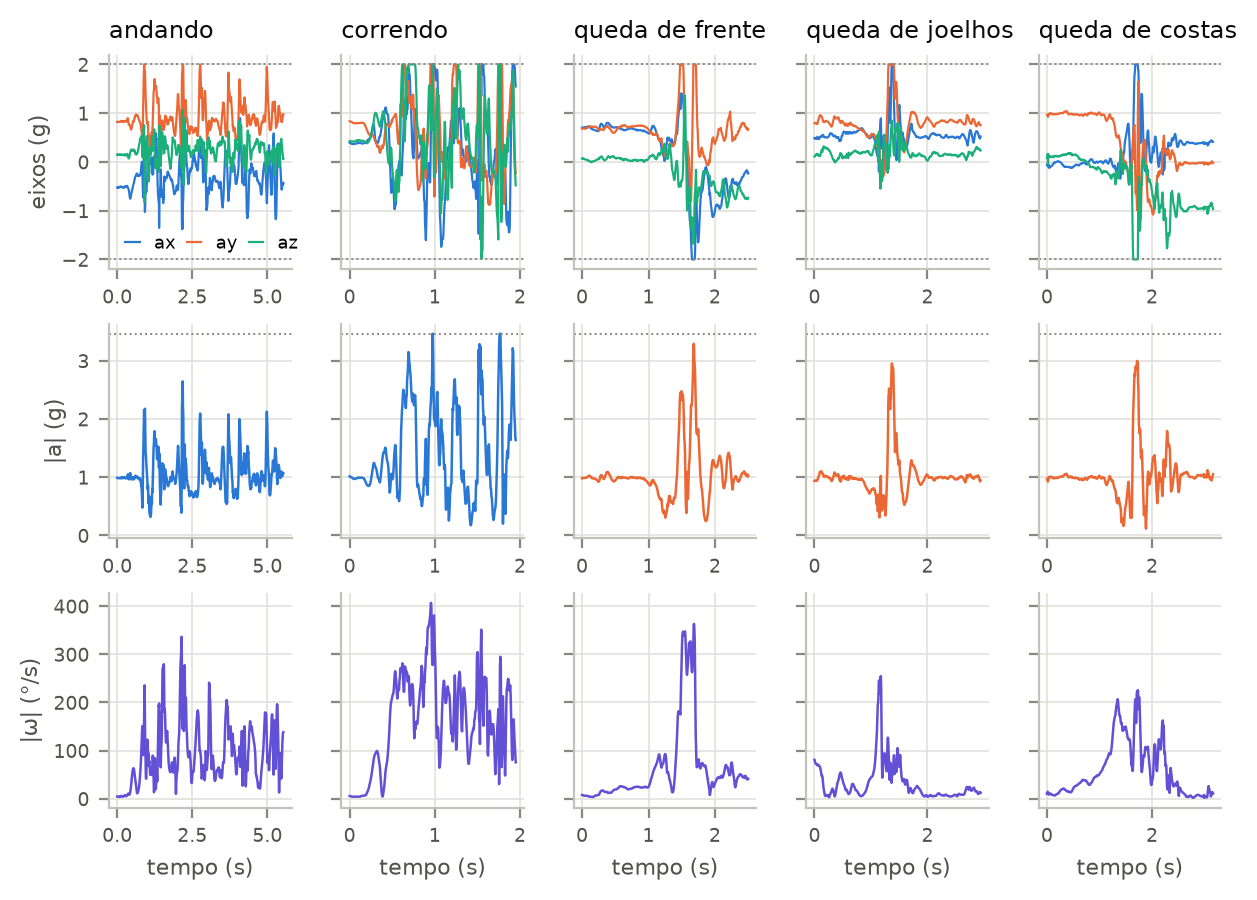
\includegraphics[width=\linewidth]{figuras/fig_mpu_cenarios.png}
\caption{Um ensaio de cada cenário do primeiro semestre (sensor na cintura, $\pm$2\,g):
os três eixos, $\amag$ e $\wmag$. As linhas pontilhadas são o teto de $\pm$2\,g por eixo e o
de 3,46\,g na magnitude. Nas quedas, o padrão é queda livre ($\amag < 1$\,g), impacto e
quietude; na corrida, picos repetidos.}
\label{fig:mpu_cenarios}
\end{figure}

\begin{figure}[H]
\centering
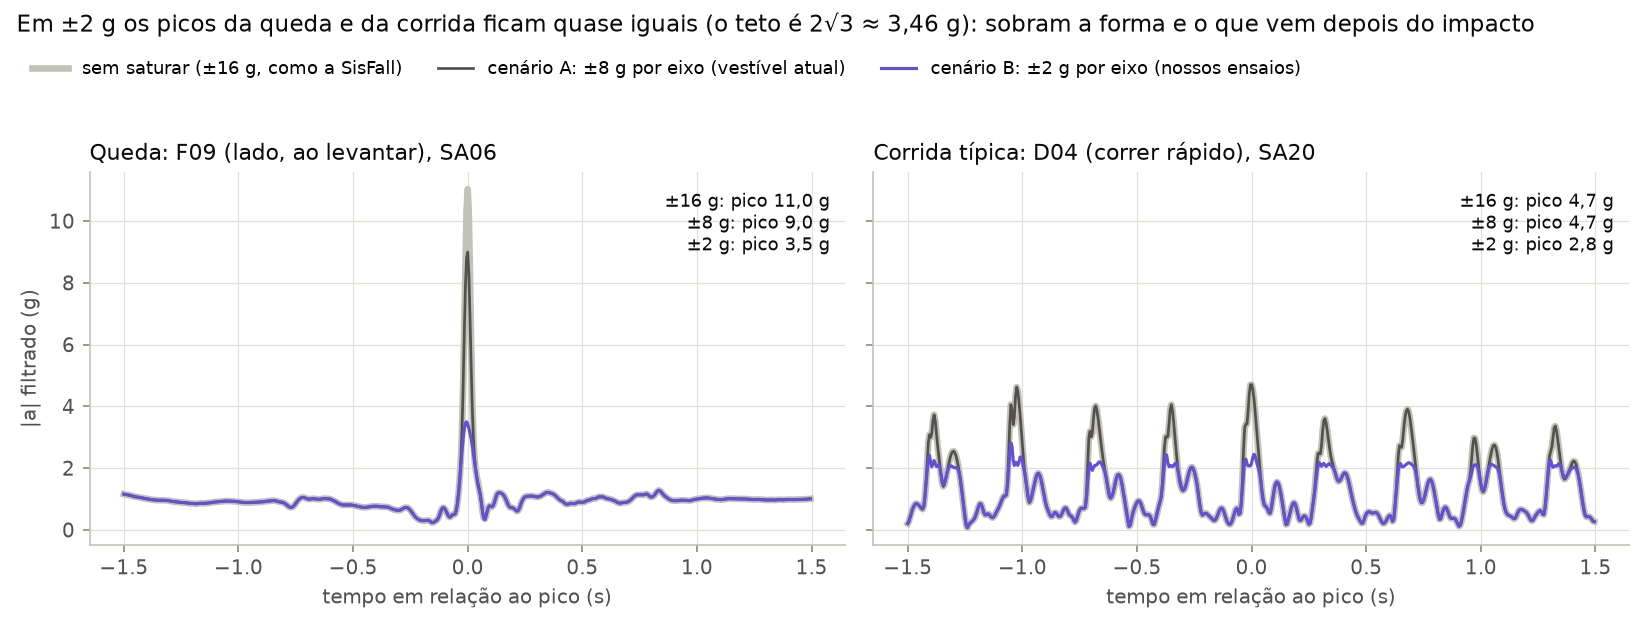
\includegraphics[width=\linewidth]{figuras/fig_saturacao.png}
\caption{Efeito da faixa do sensor em uma queda e uma corrida da SisFall: em $\pm$2\,g, os
dois picos ficam quase iguais. Reproduzida do relatório do Q1~\cite{q1}.}
\label{fig:saturacao}
\end{figure}

%----------------------------------------------------------------------
\subsection{LM35DZ: temperatura}\label{sec:lm35}

O LM35 é um sensor de temperatura integrado com saída em tensão proporcional à
temperatura em Celsius, nominalmente 10\,mV/°C, sem precisar de calibração externa para a
exatidão de catálogo~\cite{lm35}. A versão DZ (encapsulamento TO-92) mede de 0 a 100\,°C,
consome menos de 60\,µA, o que o aquece menos de 0,1\,°C no ar parado, e aceita de 4 a 30\,V.
No hub, ele é alimentado com os 5\,V da placa. A exatidão de catálogo da versão D é a mais
folgada da família (até $\pm$1,5\,°C a 25\,°C); por isso a cadeia inteira foi calibrada contra
uma referência.

\paragraph{Caracterização.} No primeiro semestre, o sensor foi aquecido numa placa
térmica, junto com um termômetro de referência, e dois multímetros leram ao mesmo tempo a
saída do LM35 e a saída do circuito de condicionamento (Figura~\ref{fig:bancada_lm35}). Foram
\lmPontos{} pontos de 0 a 62,2\,°C. O ajuste por mínimos quadrados
(Figura~\ref{fig:lm35}) dá:
\begin{equation}
  V_\text{LM35} = \lmAlfa\,\tfrac{\text{mV}}{\text{°C}}\cdot T + \lmBeta\,\text{mV}
  \qquad (R^2 = \lmRdoisSensor),
\end{equation}
\begin{equation}
  V_\text{cond} = \lmAlfaCadeia\,\tfrac{\text{mV}}{\text{°C}}\cdot T + \lmBetaCadeia\,\text{mV}
  \qquad (R^2 = \lmRdoisCadeia).
  \label{eq:cadeia}
\end{equation}

A inclinação medida no sensor ficou abaixo dos 10\,mV/°C nominais, e os resíduos têm uma
curvatura: o maior desvio é de \lmResMaxCadeia\,°C, no ponto de 0\,°C, e o desvio médio
quadrático na cadeia é de \lmResRmsCadeia\,°C. Como a curva usada no firmware é a da
\emph{cadeia completa} (Eq.~\ref{eq:cadeia}), ela já absorve o ganho real do amplificador e o
desvio do sensor. A razão entre as duas inclinações dá o ganho medido do amplificador,
$\lmAlfaCadeia/\lmAlfa = \lmGanhoMedido$.

\begin{figure}[H]
\centering
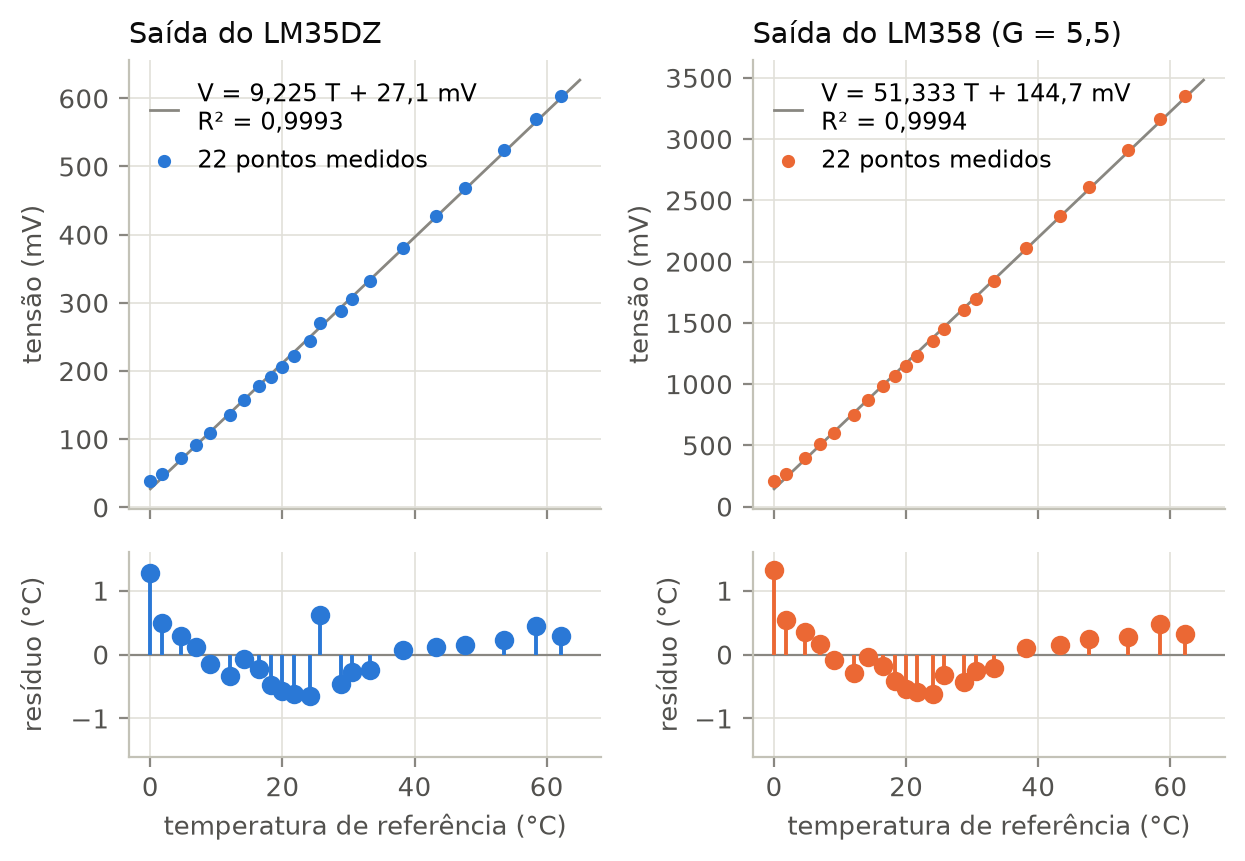
\includegraphics[width=\linewidth]{figuras/fig_lm35_caracterizacao.png}
\caption{Caracterização do LM35DZ: os \lmPontos{} pontos medidos, o ajuste por mínimos
quadrados e os resíduos convertidos em °C. Esquerda: saída do sensor; direita: saída do
condicionamento, que é a curva usada no firmware.}
\label{fig:lm35}
\end{figure}

\begin{figure}[H]
\centering
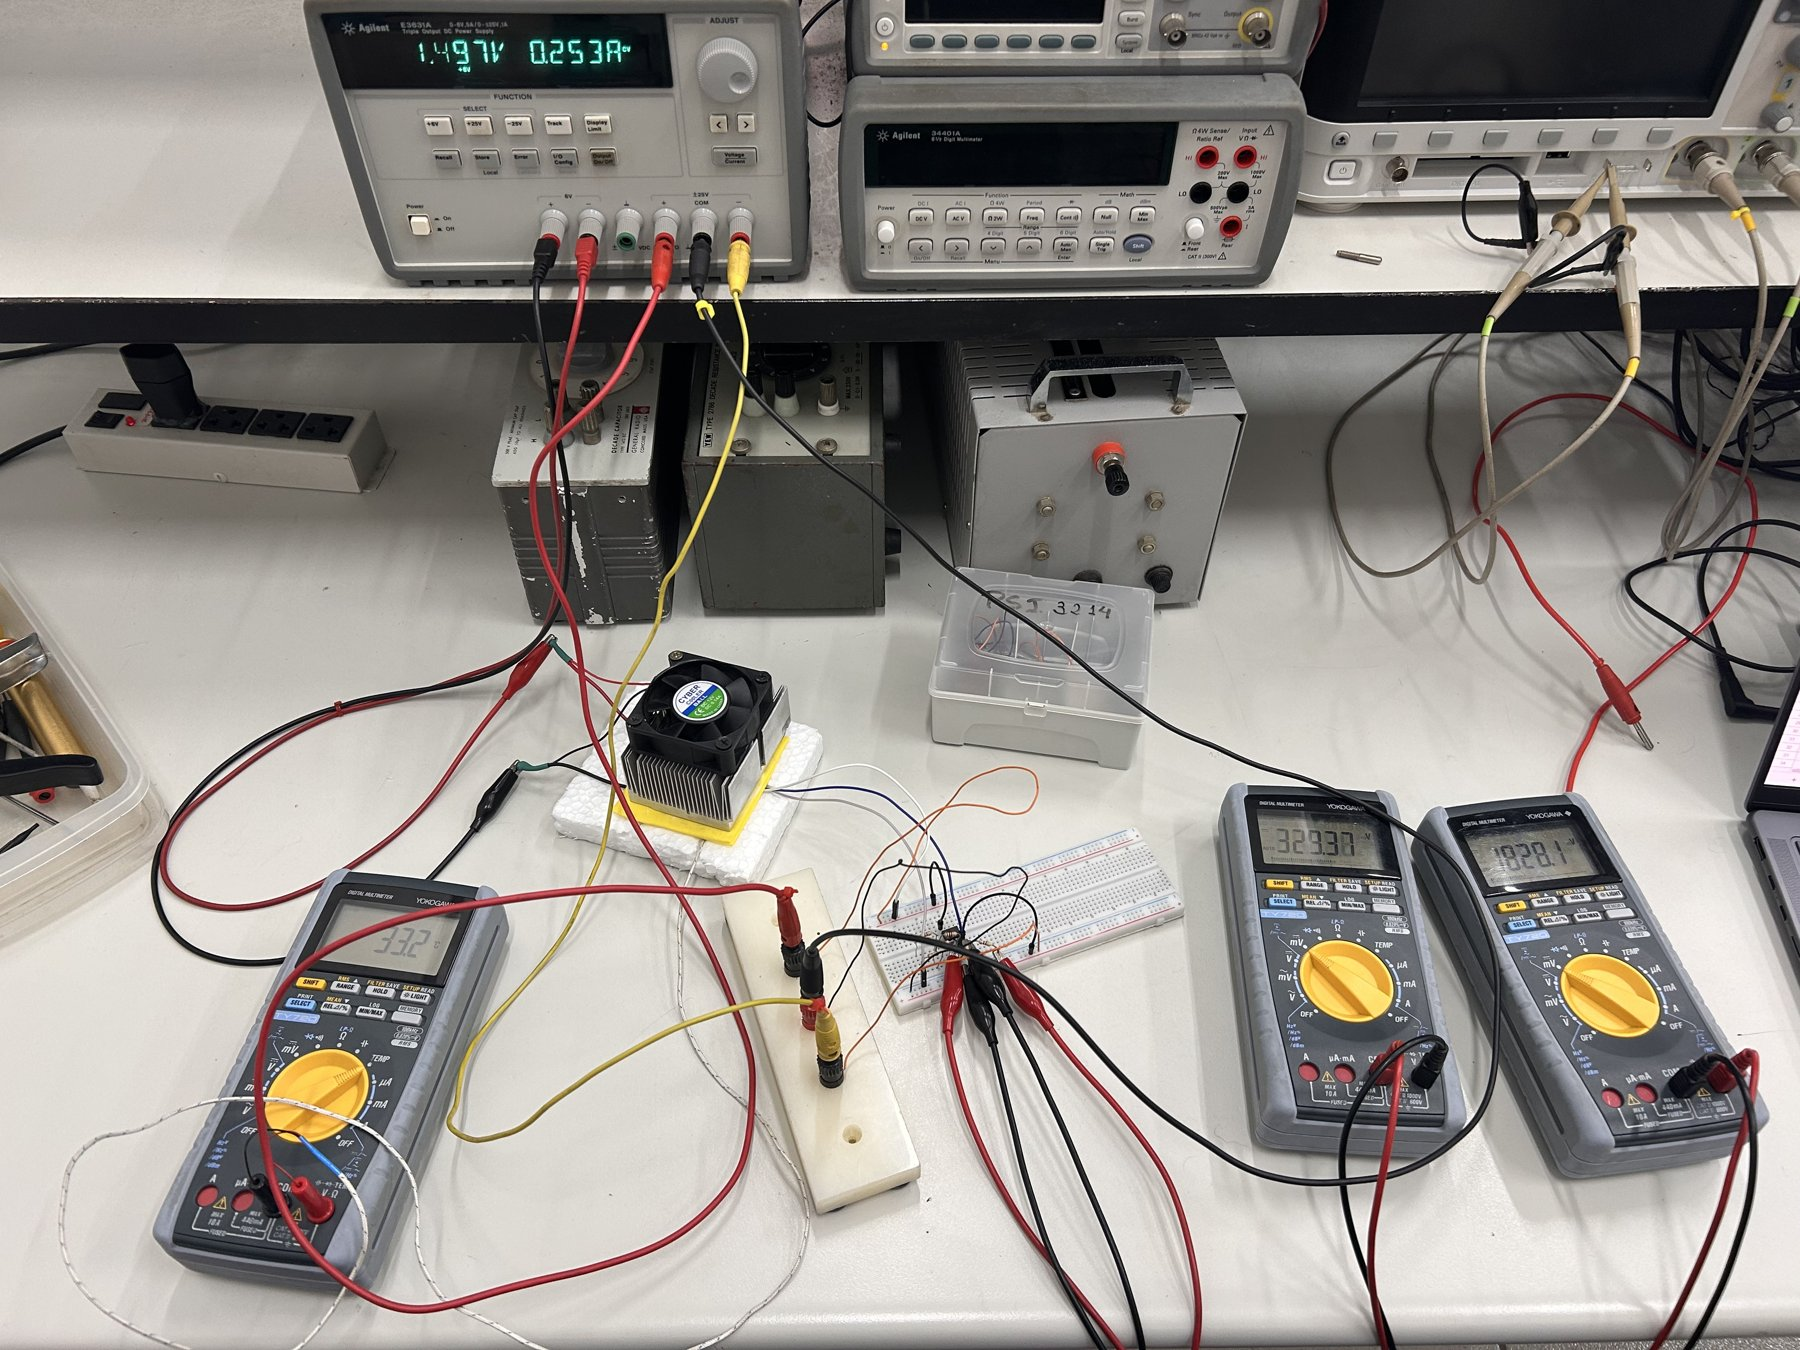
\includegraphics[width=0.78\linewidth]{imagens/s1_bancada_lm35.jpg}
\caption{Bancada da caracterização (primeiro semestre): fonte, placa térmica com o LM35 e
o termômetro de referência, protoboard com o LM358 e os multímetros lendo as duas tensões.}
\label{fig:bancada_lm35}
\end{figure}

%----------------------------------------------------------------------
\subsection{HC-SR501: presença}

O HC-SR501 é um módulo com sensor piroelétrico, lente de Fresnel e um circuito de
tratamento que entrega uma saída digital de 3,3\,V quando detecta o movimento de um corpo
quente~\cite{hcsr501}. Ele vê até cerca de 7\,m, num cone de $\sim$110°, e é alimentado com
5\,V. Dois trimpots ajustam a sensibilidade e o tempo em que a saída fica alta depois da
detecção, e um jumper escolhe o modo; usamos o modo H, em que cada novo movimento renova o
tempo.

Na prática, o sensor vê \emph{movimento}, não presença: uma pessoa dormindo, parada, não o
aciona. É por isso que a regra de inatividade só vale de dia
(Seção~\ref{sec:regras}). O módulo precisa de cerca de um minuto para estabilizar depois de
ligado, e o firmware ignora a saída nos primeiros 60\,s. Ele também tem fama de disparar
sozinho perto do Wi-Fi, o que pesou na posição dele na placa (Seção~\ref{sec:layout}). O
domo precisa sair por um furo na caixa: acrílico e vidro barram o infravermelho.

%----------------------------------------------------------------------
\subsection{MC-38: portas}

O MC-38 é um par reed switch e ímã: com a porta fechada, o ímã fica a poucos
milímetros do reed, e o contato fecha. A ligação é a mais simples possível: um terminal no
GPIO, com o \textit{pull-up} interno da ESP32, e o outro no GND. Porta fechada lê 0; porta
aberta lê 1. Isso tem uma consequência: um fio solto também lê ``aberta'', e não há como
distinguir os dois casos no sinal. Por isso as portas não instaladas são declaradas na
configuração do firmware (Seção~\ref{sec:ausente}).

O contato mecânico \textit{repica} ao fechar, e o fio até a porta funciona como antena. O
tratamento é digital (Seção~\ref{sec:cond_digital}). O hub aceita até 8 portas, uma por
identificador CAN; a placa tem conectores para duas (quarto e banheiro) e GPIOs reservados
para mais seis.

%----------------------------------------------------------------------
\subsection{Botão e LED}\label{sec:botao}

O botão da pulseira (GPIO 18) usa o \textit{pull-up} interno, um capacitor de 100\,nF em
paralelo e o filtro de \textit{glitch} do GPIO. Ele tem dois gestos, e um aperto simples não
faz nada (Tabela~\ref{tab:gestos}):
\begin{itemize}
  \item \textbf{dois toques rápidos} (``estou bem''): cancelam o alerta dos últimos 15\,s, seja
        uma queda, seja um pedido de ajuda. São dois apertos de menos de 1\,s, o segundo
        começando até 1\,s depois de soltar o primeiro;
  \item \textbf{segurar por 3\,s} (``preciso de ajuda''): fora de alerta, abre o alerta
        \code{ajuda}, que segue o mesmo caminho da queda até o cuidador. Cobre a queda que o
        modelo não detectou e qualquer outra situação em que o residente precise de alguém.
\end{itemize}

\begin{table}[H]
\centering
\caption{Gestos do botão da pulseira.}
\label{tab:gestos}
\small
\begin{tabular}{@{}>{\raggedright\arraybackslash}p{4.6cm}>{\raggedright\arraybackslash}p{2.4cm}>{\raggedright\arraybackslash}p{6.8cm}@{}}
\toprule
Estado da pulseira & Gesto & Efeito \\
\midrule
nos 15\,s depois de uma queda ou de um pedido de ajuda (LED vermelho) & dois toques & cancela esse alerta (\code{FALL\_CANCEL} ou \code{HELP\_CANCEL}) \\
normal & segurar 3\,s & pedido de ajuda (\code{HELP}), com a mesma janela de 15\,s para cancelar \\
qualquer um & aperto simples & nada \\
nos 15\,s depois de um alerta & segurar & nada: o alerta já está aberto \\
normal & dois toques & nada: não há alerta para cancelar \\
\bottomrule
\end{tabular}
\end{table}

Os gestos foram escolhidos pelo pior caso de cada um. Quem cai pode ficar deitado sobre o
braço, com o botão apertado pelo corpo; se segurar cancelasse o alerta, a queda real seria
cancelada justamente nessa hora. A pressão do corpo produz um aperto longo, nunca dois toques
separados, e por isso o cancelamento é por dois toques. Para pedir ajuda, segurar é o gesto
comum dos dispositivos de emergência: não exige precisão de tempo, o que importa para quem
tem tremor ou artrite, e uma batida ou um esbarrão não chega a 3\,s. Um pedido feito sem
querer (dormindo sobre o braço, por exemplo) é cancelado pelos mesmos dois toques e, no pior
caso, custa uma visita do cuidador; um cancelamento sem querer deixaria alguém caído sem
socorro. Os tempos são ajustáveis no \code{menuconfig}, para calibrar com os residentes.

O LED é o WS2812 da própria DevKit, controlado pelo periférico RMT. No hub, ele pisca verde a
1\,Hz em operação normal, amarelo sem broker e vermelho a 4\,Hz com um alerta aberto; na
pulseira, pisca vermelho durante os 15\,s em que um alerta pode ser cancelado, e um vermelho
lento indica que o sensor não responde. O buzzer previsto no início foi retirado em outubro:
a sinalização local fica só com o LED, e o alerta chega ao cuidador pela central.

	%======================================================================
\section{Condicionamento de sinais}\label{sec:condicionamento}
%======================================================================
Só um sensor do sistema entrega um sinal analógico: o LM35. Ele é o único que passa por
condicionamento eletrônico. Os outros entregam sinais digitais (PIR, portas, botão) ou já
digitalizados (MPU-6050), e o tratamento deles é feito no firmware, como filtro de
\textit{glitch}, \textit{debounce} e filtragem digital (Seção~\ref{sec:cond_digital}).

\subsection{Por que amplificar o LM35}

O ADC da ESP32-S3 tem 12 bits. Com a atenuação de 12\,dB, a única que cobre a saída do
amplificador, a faixa útil vai até cerca de 3,1\,V, ou seja, \adcLsb\,mV por contagem. O
LM35 entrega 10\,mV/°C: entre 0 e 57\,°C, sua saída ocupa só \lmOcupSemGanho\,\% da faixa do
ADC, e cada contagem vale \lmResolSemGanho\,°C (Figura~\ref{fig:faixa_adc}). Isso já atenderia
à resolução pedida (0,1\,°C) no papel, mas o ADC da ESP32 tem ruído e não linearidade de
várias contagens, e qualquer milivolt de ruído na trilha vira 0,1\,°C. Com um ganho de 5,5, o
sinal ocupa \lmOcupComGanho\,\% da faixa, cada contagem passa a valer \lmResolComGanho\,°C, e
o ruído que entra depois do amplificador pesa 5,5 vezes menos.

\begin{figure}[H]
\centering
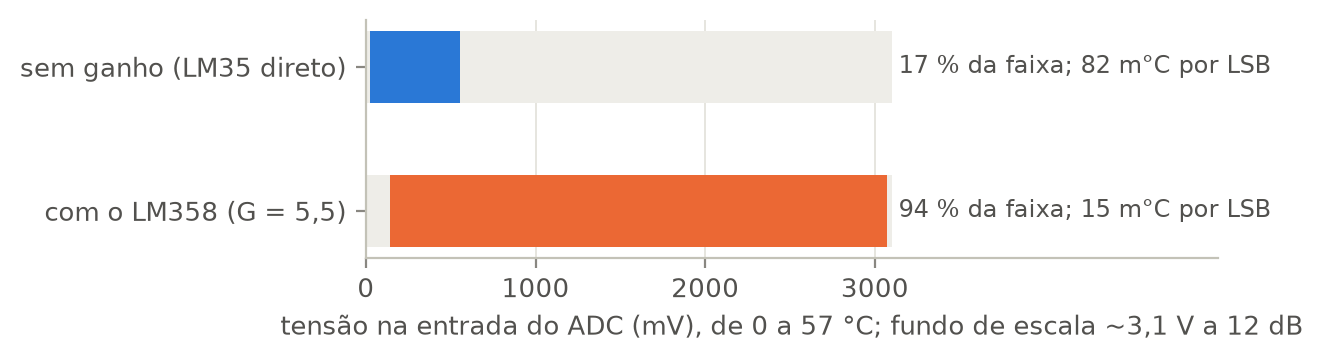
\includegraphics[width=\linewidth]{figuras/fig_lm35_faixa_adc.png}
\caption{Faixa do ADC ocupada pelo sinal de temperatura entre 0 e 57\,°C, sem e com o
amplificador, e o valor de uma contagem em °C.}
\label{fig:faixa_adc}
\end{figure}

\subsection{Circuito}

O condicionamento é um amplificador não inversor com o LM358 (Figura~\ref{fig:circuito_lm35}),
seguido de um filtro RC na entrada do ADC:
\begin{equation}
  G = 1 + \frac{R_2}{R_1} = 1 + \frac{9{,}1\,\text{k}\Omega}{2\,\text{k}\Omega} = 5{,}55 .
\end{equation}
O valor de projeto era 5,5, com $R_2 = 9$\,k$\Omega$; na série E24 o resistor mais próximo é
9,1\,k$\Omega$, compatível com o ganho medido no primeiro semestre (\lmGanhoMedido).

\begin{figure}[H]
\centering
\resizebox{0.95\linewidth}{!}{% Cadeia do LM35: sensor -> LM358 não inversor (G = 1 + R2/R1) -> filtro RC -> ADC.
\begin{circuitikz}[font=\footnotesize]
  % amplificador
  \draw (0,0) node[op amp, noinv input up] (OA) {\scriptsize U3A};
  \draw (OA.up) -- ++(0,0.5) node[above] {+5\,V};
  \draw (OA.down) -- ++(0,-0.35) node[ground] {};
  % realimentação
  \draw (OA.-) -- ++(-0.6,0) coordinate (nm);
  \draw (nm) -- ++(0,-1.4) coordinate (bot) to[R, l_={$R_2$ \SI{9.1}{\kilo\ohm}}] (bot -| OA.out) -- (OA.out);
  \draw (nm) -- ++(-1.3,0) coordinate (r1t) to[R, l_={$R_1$ \SI{2}{\kilo\ohm}}] ++(0,-2.2) node[ground] {};
  \draw (nm) node[circ] {};
  % sensor
  % na mesma altura da entrada + do amp-op, para o fio de V_out sair reto
  \node[draw, thick, minimum width=1.5cm, minimum height=1.3cm, align=center] (lm) at (OA.+ -| -5.4,0) {LM35DZ\\\scriptsize U2};
  \draw (lm.east) -- node[above, font=\scriptsize, pos=0.12] {$V_\text{out}$} (OA.+);
  \draw (lm.north) -- ++(0,0.55) coordinate (lmv) node[above] {+5\,V};
  \draw (lm.south) -- ++(0,-0.35) node[ground] {};
  \draw (lmv) ++(0,-0.25) -- ++(-1.1,0) coordinate (c1t) to[C, l_={$C_1$ \SI{100}{\nano\farad}}] ++(0,-1.9) node[ground] {};
  % saída: filtro RC e ADC
  \draw (OA.out) -- ++(0.5,0) coordinate (o) node[circ] {} to[R, l={$R_3$ \SI{10}{\kilo\ohm}}] ++(2.4,0) coordinate (g4)
        -- ++(1.0,0) node[right, align=left] {GPIO 4\\(ADC1\_CH3)};
  \draw (g4) node[circ] {} to[C, l={$C_3$ \SI{1}{\micro\farad}}] ++(0,-1.9) node[ground] {};
  \draw (o) -- ++(0,0.9) node[above, font=\scriptsize] {TP4};
\end{circuitikz}
}
\caption{Condicionamento do LM35 na PCB v1: amplificador não inversor (U3A, LM358) em
alimentação simples de 5\,V e filtro RC passa-baixa na entrada do ADC. Os capacitores de
desacoplamento ficam junto aos pinos de alimentação do LM35 (C1) e do LM358 (C2, omitido).
A outra metade do LM358 (U3B) é ligada como seguidor de 0\,V, para não oscilar.}
\label{fig:circuito_lm35}
\end{figure}

\paragraph{Alimentação simples.} No primeiro semestre, o LM358 era alimentado com $\pm$5\,V,
e o $-$5\,V vinha de um inversor na placa. Na PCB nova, ele é alimentado só com 5\,V e GND,
o que o datasheet permite (\textit{single supply}, 3 a 32\,V)~\cite{lm358}. Nessa condição,
a entrada aceita de 0 a $\sim$3,5\,V (o LM35 dá no máximo 0,6\,V) e a saída vai de
$\sim$20\,mV a $\sim$3,5\,V; o circuito usa de 0,14 a \lmVmaxCadeia\,V entre 0 e 57\,°C. Com
isso saíram da placa o inversor e suas peças, a fonte de ruído chaveada no bloco analógico e
o risco de tensão negativa num pino da ESP32.

\paragraph{Desacoplamento.} Um capacitor cerâmico de 100\,nF (X7R) junto ao pino de
alimentação do LM35 e outro junto ao do LM358, os dois ligados direto ao 5\,V da placa. Um
ramo de 5\,V separado para o analógico (ferrite ou 10\,$\Omega$ e 10\,µF) foi avaliado e
dispensado: o LM35 quase não sente o ruído da alimentação, o LM358 rejeita bem o ruído lento,
e o ruído rápido o filtro RC corta.

\subsection{Simulação e validação}\label{sec:validacao_lm358}

O circuito foi simulado em SPICE no primeiro semestre, com $G = 5{,}5$ ideal
(Figura~\ref{fig:spice}): a saída é uma reta de 0 a $\sim$3,3\,V para a entrada de 0 a 600\,mV.
Depois, ele foi montado em protoboard (Figura~\ref{fig:protoboard}) e medido junto com a
caracterização do sensor. A Tabela~\ref{tab:sim_bancada} compara a simulação e a bancada em
seis pontos da faixa.

\begin{figure}[H]
\centering
\begin{subfigure}[b]{0.49\linewidth}
  \centering
  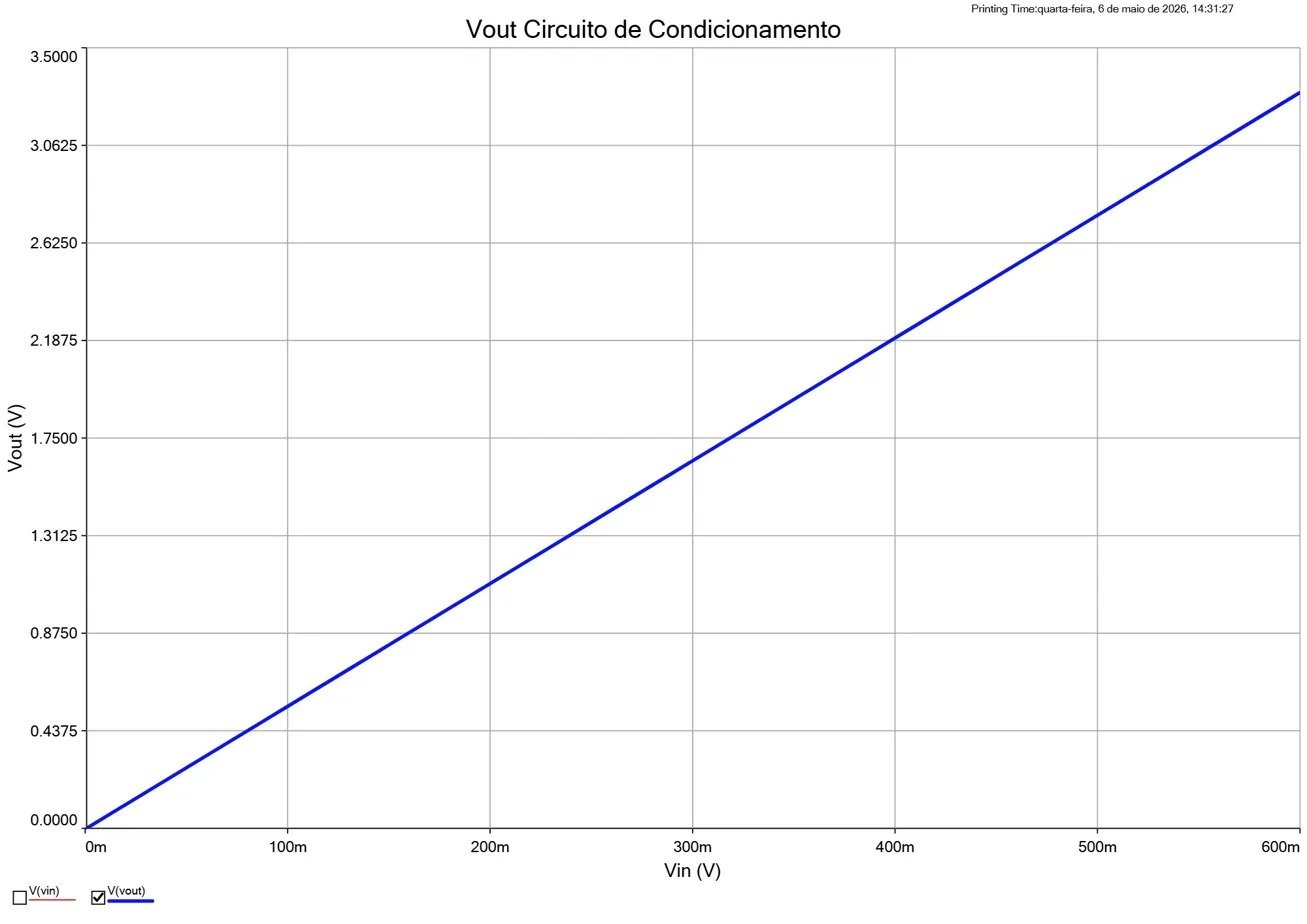
\includegraphics[width=\linewidth]{imagens/s1_spice_lm358.jpg}
  \caption{Simulação SPICE: $V_\text{out}$ em função de $V_\text{in}$.}
  \label{fig:spice}
\end{subfigure}\hfill
\begin{subfigure}[b]{0.49\linewidth}
  \centering
  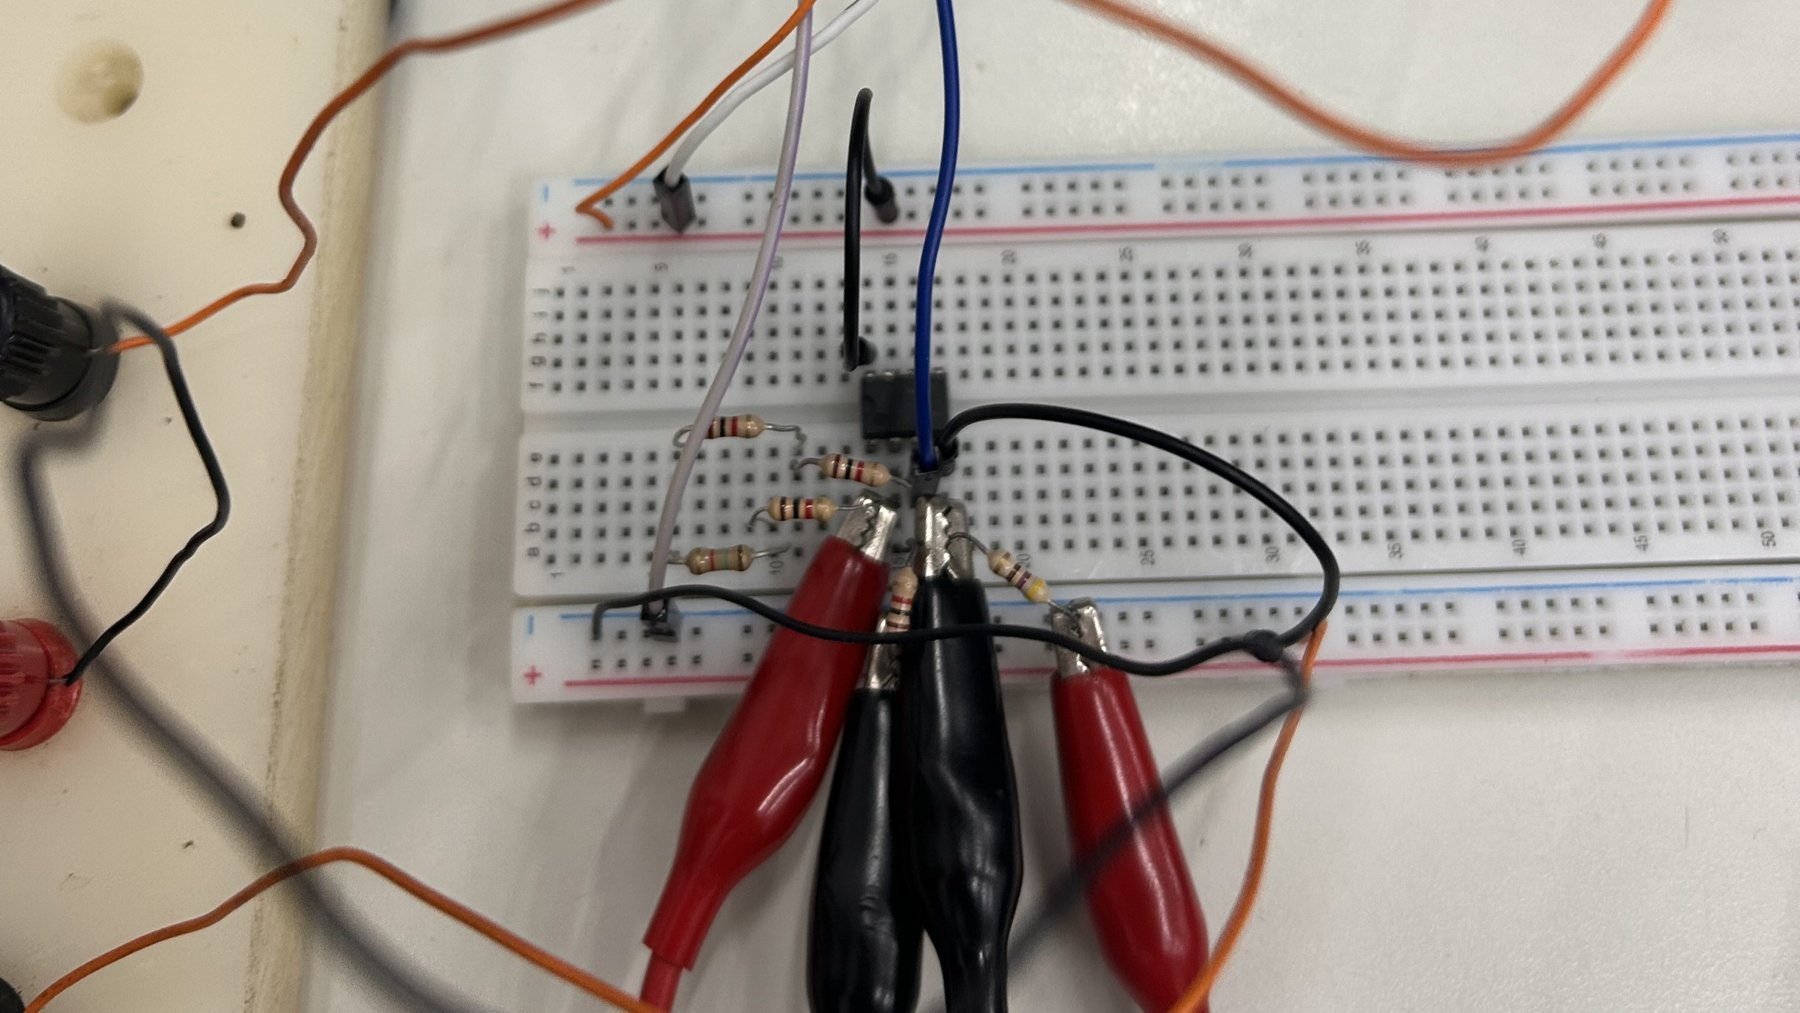
\includegraphics[width=\linewidth]{imagens/s1_protoboard_lm358.jpg}
  \caption{Montagem em protoboard.}
  \label{fig:protoboard}
\end{subfigure}
\caption{Validação do amplificador no primeiro semestre.}
\end{figure}

\begin{table}[H]
\centering
\caption{Saída prevista pela simulação ($G = 5{,}5$) e medida em bancada, para a mesma
entrada (dados do primeiro semestre).}
\label{tab:sim_bancada}
\small
\begin{tabular}{@{}S[table-format=2.1]S[table-format=3.2]S[table-format=4.2]S[table-format=4.1]S[table-format=+2.2]S[table-format=+1.2]@{}}
\toprule
{$T_\text{ref}$ (°C)} & {$V_\text{in}$ (mV)} & {$V_\text{sim}$ (mV)} & {$V_\text{med}$ (mV)} & {$\Delta$ (mV)} & {$\Delta/V_\text{med}$ (\%)} \\
\midrule
0,0  & 38,95  & 214,23  & 213,0  & -1,23  & -0,58 \\
9,0  & 108,80 & 598,40  & 602,2  & +3,80  & +0,63 \\
21,7 & 221,60 & 1218,80 & 1228,7 & +9,90  & +0,81 \\
33,3 & 332,10 & 1826,55 & 1843,6 & +17,05 & +0,93 \\
47,7 & 468,50 & 2576,75 & 2605,6 & +28,85 & +1,11 \\
62,2 & 603,60 & 3319,80 & 3354,5 & +34,70 & +1,03 \\
\bottomrule
\end{tabular}
\end{table}

O desvio cresce com a entrada e, em termos relativos, estabiliza perto de +1\,\%: é um erro
de ganho, não de \textit{offset}. O ganho real (\lmGanhoMedido) fica 1,1\,\% acima do ideal,
dentro da tolerância dos resistores. Como o firmware usa a curva medida da cadeia inteira
(Eq.~\ref{eq:cadeia}), esse erro não aparece na temperatura.

\subsection{Filtro RC na entrada do ADC}

Entre a saída do LM358 e o GPIO 4 há um resistor de 10\,k$\Omega$ em série e um capacitor
cerâmico de 1\,µF ao GND, colado no pino. É um passa-baixa de primeira ordem
(Figura~\ref{fig:rc_bode}):
\begin{equation}
  f_c = \frac{1}{2\pi R_3 C_3} = \frac{1}{2\pi \cdot 10\,\text{k}\Omega \cdot 1\,\mu\text{F}}
  \approx \rcFc\,\text{Hz}.
\end{equation}

\begin{itemize}
  \item Atenua \rcSessenta\,dB em 60\,Hz (a rede elétrica) e \rcMil\,dB em 1\,kHz, e fica abaixo
        do Nyquist das rajadas do firmware (amostras a cada 10\,ms, ou seja, 50\,Hz). A
        temperatura muda em minutos e passa inteira.
  \item Acomoda em $\sim$\rcAssentaMs\,ms ($5\tau$), muito menos que o intervalo de 60\,s entre
        medições.
  \item O capacitor fornece a carga que o capacitor de amostragem do ADC puxa a cada
        conversão, o papel do \textit{bypass} de 100\,nF recomendado pela documentação do
        ESP-IDF~\cite{espidf}.
  \item O resistor protege o pino: limita a corrente se a saída sair da faixa (ao ligar a
        placa, com o LM35 em mau contato, ou com uma ponta de prova no 5\,V). A queda nele é
        desprezível, porque só passa a corrente de fuga do pino, da ordem de nA.
  \item O capacitor é cerâmico (X7R): um eletrolítico tem fuga de µA, que nos 10\,k$\Omega$
        daria dezenas de mV de erro.
\end{itemize}

\begin{figure}[H]
\centering
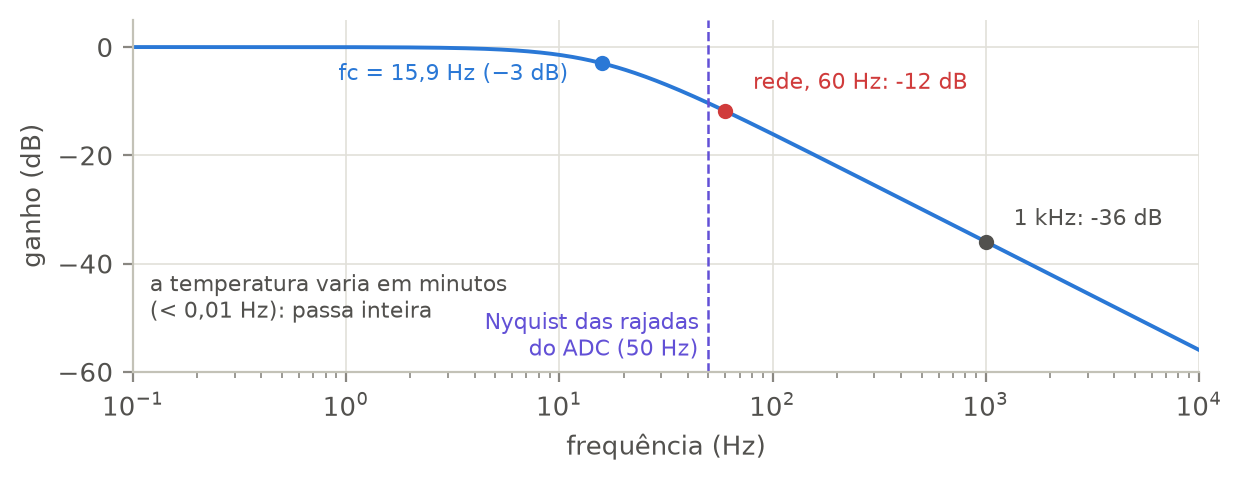
\includegraphics[width=\linewidth]{figuras/fig_rc_bode.png}
\caption{Resposta em frequência do filtro RC de 10\,k$\Omega$ e 1\,µF.}
\label{fig:rc_bode}
\end{figure}

\subsection{Aquisição da temperatura}

A cada 60\,s, a tarefa do LM35 faz 16 leituras do ADC1, canal 3 (GPIO 4), espaçadas de
10\,ms. Uma leitura por minuto basta: o ar do quarto leva dezenas de minutos para mudar, o
próprio LM35 leva minutos para acompanhá-lo, e a regra de temperatura espera 10\,min fora da
faixa. Toda leitura vai para a regra, mas só é publicada quando muda (Seção~\ref{sec:mqtt}). Cada leitura passa pela calibração do próprio chip (\code{adc\_cali}, que converte a
contagem em mV usando os parâmetros gravados de fábrica) e as 16 são promediadas, o que reduz
o ruído aleatório por um fator de $\sqrt{16} = 4$. A temperatura sai da curva da cadeia:
\begin{equation}
  T = \frac{V_\text{mV} - \lmBetaCadeia}{\lmAlfaCadeia} .
\end{equation}
Uma leitura fora de 0 a 57\,°C (o limite do ADC) é tratada como sensor solto: não é
publicada nem alimenta as regras, e o firmware avisa uma vez no log.

\subsection{Condicionamento digital dos outros sensores}\label{sec:cond_digital}

\paragraph{Portas e PIR.} Os dois são entradas digitais com interrupção nas duas bordas. Em
cada pino, o \textbf{filtro de \textit{glitch}} do GPIO da ESP32-S3 descarta pulsos mais curtos
que dois ciclos do relógio do IO-MUX: os picos captados pelos fios longos até a porta nem
chegam a gerar interrupção. O \textbf{\textit{debounce}} é por estabilização: a interrupção só
avisa que algo mudou, e a tarefa dos sensores lê o nível depois de 50\,ms sem nenhuma borda.
Assim, o repique do reed vira uma única transição, com o estado final. Na saída do PIR há um
resistor de 1\,k$\Omega$ em série (R4), que limita a corrente entre o módulo de 5\,V e o pino.

\paragraph{Botão.} \textit{Pull-up} interno, 100\,nF em paralelo e o filtro de
\textit{glitch}. O \textit{debounce} também é por estabilização, em 30\,ms: a interrupção pega
as duas bordas e só acorda a task do botão, que lê o nível quando a linha fica quieta. Um
bloqueio fixo depois de cada aperto, como os 300\,ms usados antes, engoliria o segundo toque
dos dois toques (Seção~\ref{sec:botao}).

\paragraph{MPU-6050.} O sinal inercial passa por dois filtros. O primeiro é o DLPF do próprio
sensor, em 44\,Hz, antes da decimação para 200\,Hz. O segundo é um passa-baixa Butterworth de
segunda ordem, em \bqFc\,Hz, aplicado aos 6 eixos na pulseira (Figura~\ref{fig:biquad}). Ele é um
\textit{biquad} da biblioteca ESP-DSP (\code{dsps\_biquad\_f32}), com os coeficientes
$\{b_0; b_1; b_2; a_1; a_2\} = \{\bqCoefs\}$, gerados pelo mesmo código Python que treina o
modelo de queda. Assim, o firmware filtra exatamente como o treino filtrou. Os movimentos do
corpo ficam abaixo de $\sim$12\,Hz e passam inteiros; o filtro tira o ruído e a vibração que
não ajudam a reconhecer uma queda.

\begin{figure}[H]
\centering
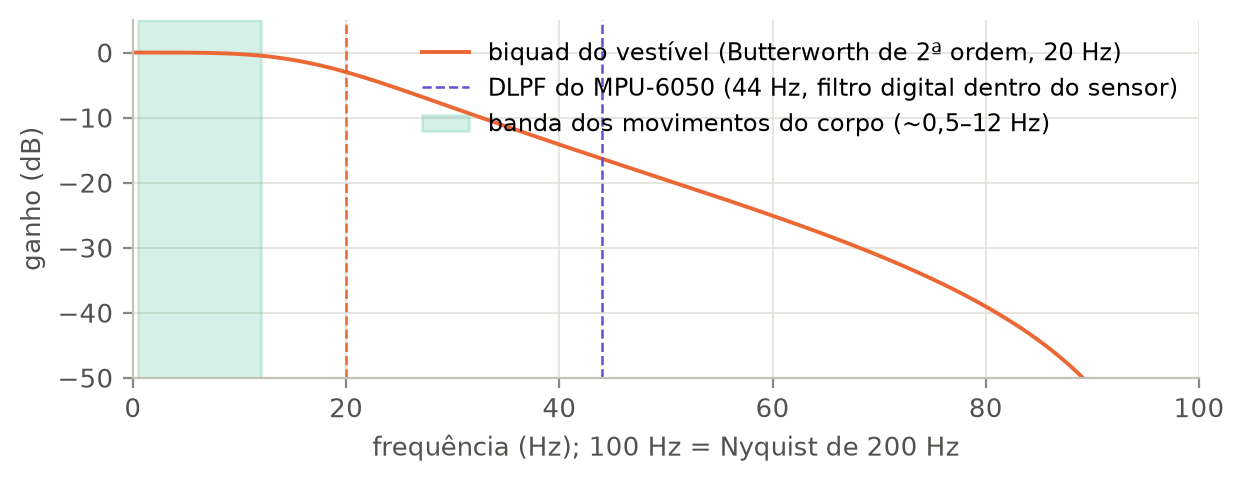
\includegraphics[width=\linewidth]{figuras/fig_biquad.png}
\caption{Resposta em frequência do passa-baixa de \bqFc\,Hz da pulseira ($f_s = \bqFs$\,Hz).}
\label{fig:biquad}
\end{figure}

	%======================================================================
\section{Hardware e placa de circuito impresso}\label{sec:pcb}
%======================================================================
\subsection{Plataforma: ESP32-S3-DevKitC-1}

As duas placas usam a ESP32-S3-DevKitC-1~\cite{esp32s3}. O ESP32-S3 tem dois núcleos
Xtensa LX7 de até 240\,MHz, 512\,KB de SRAM, Wi-Fi de 2,4\,GHz e Bluetooth LE, dois ADCs de
12 bits, o controlador CAN do próprio chip (TWAI), o periférico RMT que acende o LED
WS2812 e um coprocessador de ultrabaixo consumo (ULP RISC-V). A DevKit traz o módulo com a
antena, o regulador de 3,3\,V, uma ponte USB--serial e a USB nativa do chip. Os dois núcleos
pesaram na escolha: o rádio e os protocolos ficam num núcleo e o tempo real (amostragem,
sensores) no outro (Seção~\ref{sec:tasks}).

\subsection{Uma PCB para as duas placas}

O hub e a pulseira usam \textbf{uma só PCB}: uma placa-base em que a DevKit é encaixada e
que leva os periféricos dos dois. Só o firmware muda: o hub usa as portas, o PIR e o LM35; a
pulseira usa o MPU-6050 e o botão; os dois podem usar o CAN e o LED da DevKit
(Figura~\ref{fig:pcb_blocos}).

A placa é única por duas razões. A disciplina imprime um único modelo de placa por grupo, então
as duas placas do sistema tinham de caber num mesmo projeto. E, por ser um protótipo, juntar o
hub e a pulseira numa placa só não atrapalha os testes: as duas funções usam a mesma DevKit,
nenhuma divide pino com a outra, e o firmware escolhe o que cada uma liga.

\begin{figure}[H]
\centering
\resizebox{\linewidth}{!}{% Blocos da PCB única: o que cada placa usa em volta da DevKit.
\begin{tikzpicture}[font=\scriptsize]
  \node[draw=black!70, fill=black!5, thick, rounded corners=2pt, minimum width=3.0cm, minimum height=6.6cm,
        align=center, font=\footnotesize] (dk) at (0,0) {\textbf{ESP32-S3}\\\textbf{DevKitC-1}\\(U1, encaixada)\\[4pt]LED WS2812\\(GPIO 38/48)};

  % lado esquerdo (J1 da DevKit): analógico e entradas do quarto, CAN, alimentação
  \tikzset{esq/.style={bloco=#1, text width=4.3cm, align=left, anchor=east}, dir/.style={bloco=#1, text width=4.1cm, align=left, anchor=west}}
  \node[esq=corhub] (an) at (-2.6,2.4) {\textbf{GPIO 4}: LM35DZ $\to$ LM358 (G = 5,55) $\to$ filtro RC (U2, U3, R1--R3, C3)};
  \node[esq=corhub] (pir) at (-2.6,1.0) {\textbf{GPIO 8}: PIR HC-SR501 (J2), com R4 em série};
  \node[esq=corhub] (portas) at (-2.6,-0.2) {\textbf{GPIO 11, 12}: portas 1 e 2, reed MC-38 (J3, J4)};
  \node[esq=corambas] (can) at (-2.6,-1.6) {\textbf{GPIO 13, 14}: transceptor CAN SN65HVD230 (J1) e barramento CANH, CANL, GND (J7)};
  \node[esq=cinza] (pwr) at (-2.6,-3.0) {\textbf{5V}: USB-C (J6) $\to$ C8 $\to$ D1 1N5819};
  % lado direito (J3 da DevKit): I2C, botão, pontos de teste
  \node[dir=corvest] (mpu) at (2.6,2.0) {\textbf{GPIO 1, 2 (I²C) e 17 (INT)}: MPU-6050 (J5); par do ULP, INT em RTC GPIO};
  \node[dir=corvest] (bt) at (2.6,0.5) {\textbf{GPIO 18}: botão ``estou bem'' (SW1)};
  \node[dir=cinza] (tp) at (2.6,-1.0) {pontos de teste: 5V, 3V3, GND, saída do LM358, CANH, CANL};
  \node[dir=cinza] (livre) at (2.6,-2.5) {livres: 6, 7 (analógico), 9, 10 (portas 3 e 4), 21 e 39--42 (expansão)};

  \foreach \n in {an,pir,portas,can,pwr} {\draw[thick, black!60] (\n.east) -- (\n.east -| dk.west);}
  \foreach \n in {mpu,bt,tp,livre} {\draw[thick, black!60] (\n.west) -- (\n.west -| dk.east);}

  % legenda
  \node[anchor=north, align=left, font=\scriptsize] at (0,-3.7) {%
    \tikz\fill[corhub!40] (0,0) rectangle (0.3,0.2); só o hub \quad
    \tikz\fill[corvest!40] (0,0) rectangle (0.3,0.2); só a pulseira \quad
    \tikz\fill[corambas!40] (0,0) rectangle (0.3,0.2); os dois (na pulseira, só em bancada) \quad
    \tikz\fill[cinza!40] (0,0) rectangle (0.3,0.2); comum};
\end{tikzpicture}
}
\caption{Blocos da PCB v1 em volta da DevKit, com o GPIO de cada um.}
\label{fig:pcb_blocos}
\end{figure}

\subsection{Mapa de pinos}\label{sec:pinos}

Como as duas placas compartilham a PCB, nenhuma função divide pino com outra. A escolha
seguiu regras tiradas da documentação do ESP-IDF para o ESP32-S3 e da aula de projeto de
PCB (Tabela~\ref{tab:regras_pinos}): não usar um pino que uma função do chip ligada no futuro
tomaria, mesmo que hoje não haja conflito.

\begin{table}[H]
\centering
\caption{Regras de escolha dos pinos.}
\label{tab:regras_pinos}
\small
\begin{tabular}{@{}l>{\raggedright\arraybackslash}p{2.0cm}>{\raggedright\arraybackslash}p{10.2cm}@{}}
\toprule
Nível & GPIO & Por quê \\
\midrule
nunca & 0, 3, 45, 46 & pinos de \textit{strapping}: o nível no boot muda o modo da placa \\
nunca & 19, 20 & USB nativa (console, gravação, depuração) \\
nunca & 43, 44 & UART0: o console e a gravação pela ponte USB da DevKit \\
nunca & 26--37 & memória flash e, nos módulos com PSRAM octal, a PSRAM \\
nunca & 38, 47, 48 & LED RGB da DevKit (38 ou 48, conforme a versão) e o par 47/48, alimentado em 1,8\,V em alguns módulos \\
reserva & 15, 16 & cristal de 32\,kHz, para um relógio preciso em \textit{light sleep} na pulseira \\
expansão & 39--42 & JTAG por pinos; o que ficar aqui se perde se ele for ligado \\
analógico & 1--10 & só o ADC1: o ADC2 não funciona com o Wi-Fi ligado \\
I²C & 1 (SDA), 2 (SCL) & o único par que o I²C do coprocessador ULP aceita fora dos pinos de \textit{strapping}: o ULP poderá ler o MPU em \textit{deep sleep} sem refazer a placa \\
acordar & 0--21 & o botão e a interrupção do MPU precisam ser RTC GPIO para acordar a pulseira \\
\bottomrule
\end{tabular}
\end{table}

O mapa resultante está na Tabela~\ref{tab:pinos} e, completo, no Apêndice~\ref{ap:pinos}. No
firmware, ele fica num arquivo só (\code{pcb\_pins.h}), \textbf{verificado na compilação}: o
build falha se dois sinais caírem no mesmo GPIO, se algum cair num pino proibido ou reservado,
ou se um sinal analógico sair do ADC1. A PCB do primeiro semestre tinha quatro desses
conflitos (Seção~\ref{sec:pcb_s1}).

\begin{table}[H]
\centering
\caption{Pinos usados na PCB v1.}
\label{tab:pinos}
\small
\begin{tabular}{@{}l>{\raggedright\arraybackslash}p{5.4cm}l>{\raggedright\arraybackslash}p{4.6cm}@{}}
\toprule
GPIO & Função & Placa & Observação \\
\midrule
1, 2 & I²C SDA, SCL (MPU-6050) & pulseira & par do ULP \\
4 & LM35 (saída do LM358) & hub & ADC1, canal 3 \\
8 & PIR HC-SR501 & hub & \\
11, 12 & portas 1 (quarto) e 2 (banheiro) & hub & digitais: o ADC2 não importa \\
13, 14 & CAN TX, RX & os dois & na pulseira, só em bancada \\
17 & interrupção do MPU-6050 & pulseira & RTC GPIO \\
18 & botão ``estou bem'' & pulseira & RTC GPIO \\
38 ou 48 & LED WS2812 & os dois & é o da DevKit \\
\bottomrule
\end{tabular}
\end{table}

\subsection{Alimentação}\label{sec:alimentacao}

A placa tem uma entrada só, um módulo USB-C, e não carrega bateria
(Figura~\ref{fig:alimentacao}). O hub usa um carregador de tomada; a pulseira, no protótipo,
um \textit{power bank}. Como só há uma entrada, nunca há duas fontes juntas.

\begin{figure}[H]
\centering
\resizebox{0.92\linewidth}{!}{% Entrada de alimentação da PCB: módulo USB-C -> +5V -> D1 -> DevKit; periféricos de 5 V direto.
\begin{circuitikz}[font=\footnotesize]
  \node[draw, thick, minimum width=1.9cm, minimum height=2.0cm, align=center] (usb) at (0,0) {módulo\\USB-C\\(J6)};
  \draw ($(usb.east)+(0,0.5)$) node[anchor=south west, font=\tiny] {V} -- ++(2.0,0) coordinate (v5) node[circ] {} node[above] {+5V};
  \draw ($(usb.east)+(0,-0.5)$) node[anchor=north west, font=\tiny] {G} -- ++(0.6,0) -- ++(0,-0.4) node[ground] {};
  \draw (v5) to[C, l={$C_8$ \SI{10}{\micro\farad}}] ++(0,-2.0) node[ground] {};
  \draw (v5) -- ++(1.4,0) coordinate (n1) node[circ] {} to[D, l={$D_1$ 1N5819}] ++(2.4,0) coordinate (dk)
        -- ++(0.6,0) node[right, align=left] {pino 5V da DevKit\\(o regulador de 3,3\,V dela alimenta\\o MPU-6050 e o transceptor CAN)};
  \draw (n1) -- ++(0,1.2) -- ++(3.0,0) node[right, align=left] {LM35, LM358 e PIR (5\,V)};
\end{circuitikz}
}
\caption{Entrada de alimentação da PCB v1.}
\label{fig:alimentacao}
\end{figure}

\begin{itemize}
  \item \textbf{C8 (10\,µF)}, junto ao conector, segura a tensão nos picos de corrente do
        rádio.
  \item \textbf{D1 (1N5819, Schottky)} leva o 5\,V ao pino 5V da DevKit e impede que a
        entrada da placa e a USB da DevKit, ligada para gravar, fiquem em paralelo. A queda
        de um Schottky ($\sim$0,3\,V) não atrapalha o regulador de 3,3\,V da DevKit.
  \item O LM35, o LM358 e o PIR são alimentados direto no 5\,V da placa; o MPU-6050 e o
        transceptor CAN, nos 3,3\,V do regulador da DevKit.
  \item O módulo USB-C usado não tem os resistores de 5,1\,k$\Omega$ nos pinos CC, que
        pedem 5\,V a uma fonte USB-C. Por isso a placa só liga com cabo USB-A $\to$ C,
        como confirmado num teste em 23/10.
\end{itemize}

\paragraph{Consumo.} A estimativa para a pulseira com o rádio ligado é de 110 a 130\,mA,
o que daria de 20 a 25\,h com um \textit{power bank} de 5000\,mAh. Muitos \textit{power banks} desligam sozinhos abaixo de 50 a 100\,mA, o
que vai importar quando o \textit{light sleep} baixar o consumo. Sem medição de bateria nesta
placa, a pulseira informa a bateria como desconhecida, e o alerta de bateria baixa fica
desligado.

\subsection{Esquemático}

O esquemático foi feito no KiCad 10, em folhas hierárquicas: a folha principal com a DevKit
e uma folha por bloco (LM35, CAN, PIR, cada porta, botão, MPU-6050 e entrada USB-C). A
Figura~\ref{fig:esquema_raiz} mostra a folha principal; as demais estão no
Apêndice~\ref{ap:esquema}.

\begin{figure}[H]
\centering
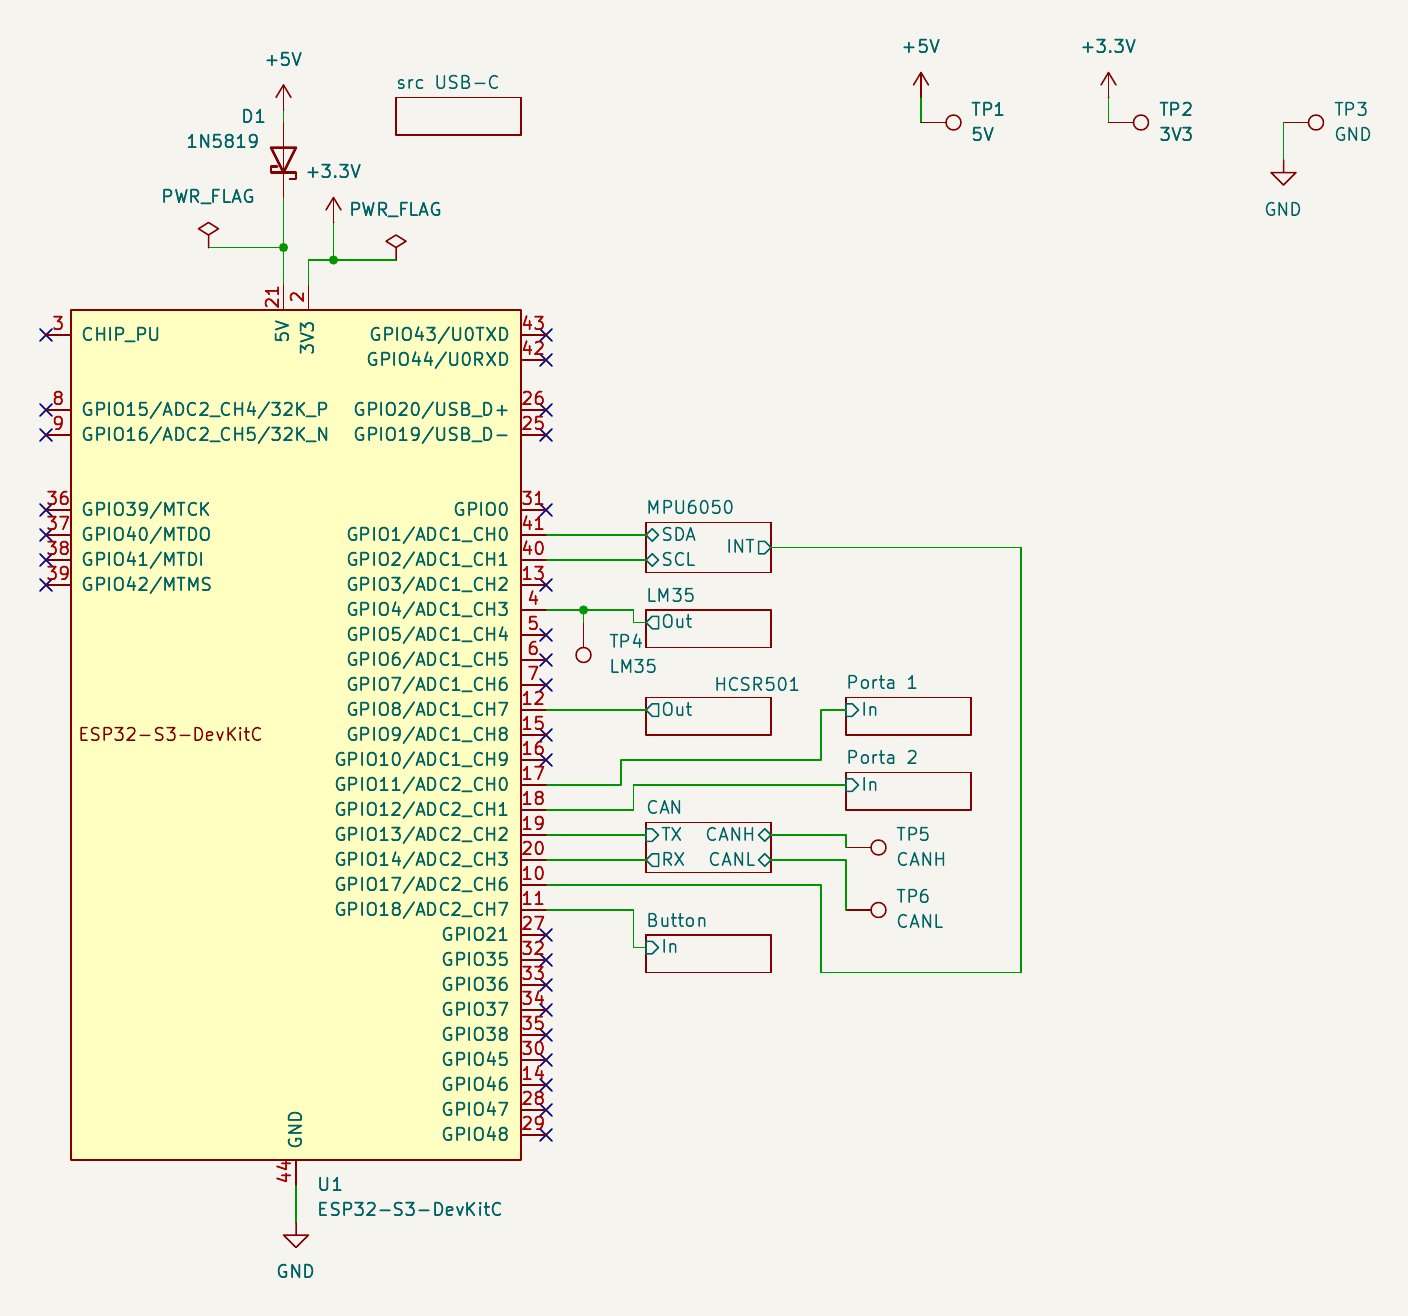
\includegraphics[width=0.9\linewidth]{figuras/esquema_p1.png}
\caption{Folha principal do esquemático: a DevKit (U1) e os blocos ligados aos seus pinos.}
\label{fig:esquema_raiz}
\end{figure}

\subsection{Layout}\label{sec:layout}

A placa mede \pcbLargura{} $\times$ \pcbAltura\,mm e tem duas camadas: as trilhas na face de
cima (F.Cu) e um plano de GND quase inteiro na de baixo (B.Cu), com alívio térmico nos
furos (Figuras~\ref{fig:pcb_3d} e~\ref{fig:pcb_camadas}). Os componentes são todos de furo
passante, para montagem à mão, e os módulos (DevKit, PIR, MPU, transceptor CAN, USB-C) entram
em barras de pinos fêmea. As decisões de posicionamento vieram da aula de projeto de PCB:

\begin{itemize}
  \item \textbf{Bloco analógico separado.} O LM35, o LM358 e o filtro RC ficam juntos, do
        lado do GPIO 4, longe do transceptor CAN e do I²C. A trilha do LM35 até o LM358 é
        curta, porque é o sinal pequeno (10\,mV/°C), e o RC fica colado no pino do ADC.
  \item \textbf{LM35 longe do calor.} Ele fica numa ponta da placa, longe da DevKit e do
        regulador, que esquentam com o Wi-Fi.
  \item \textbf{Antena livre.} Não há cobre embaixo da antena da DevKit, nas duas faces: o
        retângulo vazio no plano de GND da Figura~\ref{fig:pcb_camadas}.
  \item \textbf{PIR longe da antena}, na metade oposta da placa, por causa dos disparos falsos
        do HC-SR501 perto do Wi-Fi. O módulo fica deitado sobre a placa, com o domo para fora.
  \item \textbf{Plano de terra contínuo}, com o mínimo de fendas sob as trilhas de sinal, e
        100\,nF em cada pino de alimentação de CI.
\end{itemize}

\begin{figure}[H]
\centering
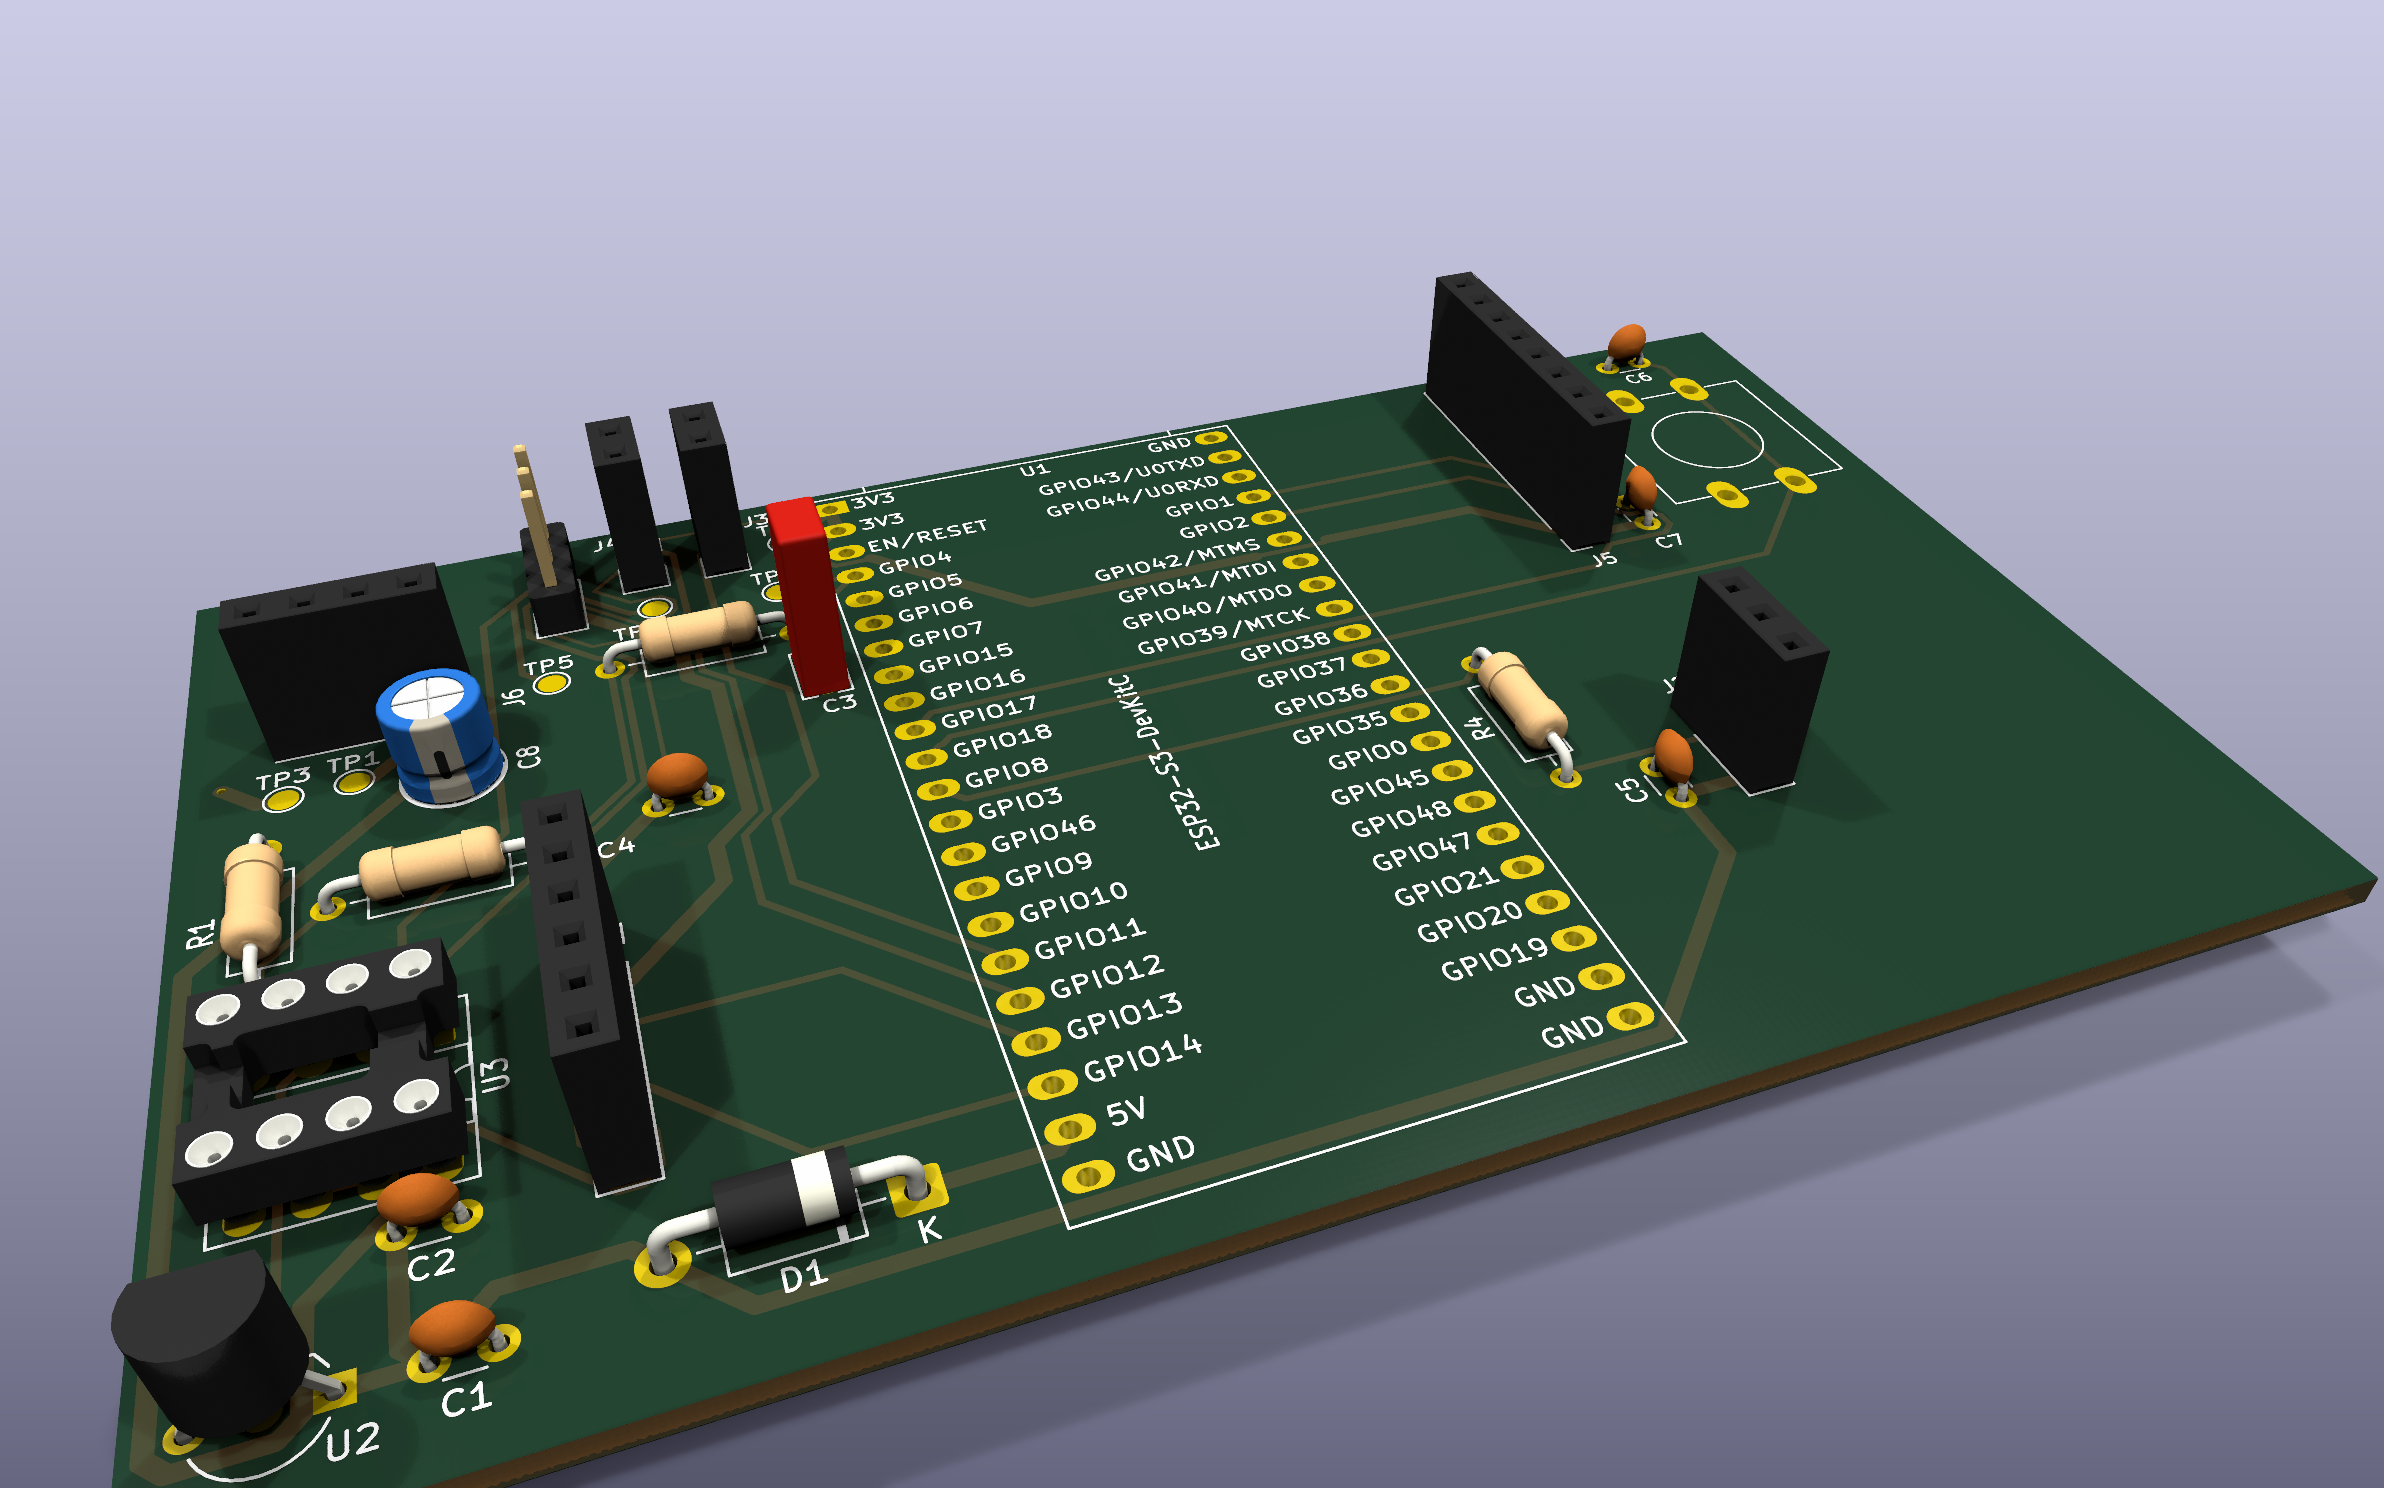
\includegraphics[width=0.9\linewidth]{figuras/pcb_3d_perspectiva.png}
\caption{Visualização 3D da PCB v1 (KiCad). O LM35 e o LM358 estão no canto de baixo à
esquerda; a DevKit, ao centro; o MPU-6050 e o botão, à direita.}
\label{fig:pcb_3d}
\end{figure}

\begin{figure}[H]
\centering
\begin{subfigure}[b]{0.49\linewidth}
  \centering
  \camada{\pcbTrimF}{\linewidth}{figuras/pcb_fcu.pdf}
  \caption{Face de cima: trilhas (F.Cu) e serigrafia.}
\end{subfigure}\hfill
\begin{subfigure}[b]{0.49\linewidth}
  \centering
  \camada{\pcbTrimB}{\linewidth}{figuras/pcb_bcu.pdf}
  \caption{Face de baixo (B.Cu), vista por baixo: plano de GND.}
\end{subfigure}
\caption{Camadas de cobre da PCB v1, exportadas do KiCad.}
\label{fig:pcb_camadas}
\end{figure}

\paragraph{Regras de projeto.} As regras ficam com folga sobre os limites da JLCPCB para
duas camadas (0,127\,mm de trilha e afastamento), pensando numa placa soldada à mão
(Tabela~\ref{tab:regras_pcb}).

\begin{table}[H]
\centering
\caption{Regras de projeto da PCB v1.}
\label{tab:regras_pcb}
\small
\begin{tabular}{@{}>{\raggedright\arraybackslash}p{6.2cm}>{\raggedright\arraybackslash}p{7.6cm}@{}}
\toprule
Item & Valor \\
\midrule
Afastamento e trilha mínimos & 0,2\,mm e 0,2\,mm \\
Trilhas de sinal & 0,4\,mm (0,25\,mm só em trecho apertado), afastamento de 0,25\,mm \\
Trilhas de alimentação (5\,V, 3,3\,V, GND) & 0,8\,mm; o pico de corrente é de $\sim$0,5\,A \\
Via & 0,8\,mm de diâmetro com furo de 0,4\,mm \\
Cobre até a borda & 0,5\,mm \\
Pads da DevKit & furo de 1,0\,mm, pad oval de 1,4 $\times$ 2,2\,mm: a barra de pinos tem 0,9\,mm de diagonal e não entrava no furo de 0,8\,mm do footprint original \\
Pads do LM35 & TO-92 de pads largos (1,5\,mm), para soldar à mão \\
Empilhamento & FR-4 de 1,6\,mm, cobre de 1\,oz (35\,µm) \\
\bottomrule
\end{tabular}
\end{table}

\subsection{Verificação e fabricação}

Antes de gerar os arquivos de fabricação, a placa passou por:
\begin{itemize}
  \item \textbf{ERC} (regras elétricas do esquemático): \ercViolacoes{} violações.
  \item \textbf{DRC} (regras de projeto do layout), com paridade com o esquemático:
        \drcErros{} erros, \drcSemLigacao{} ligações faltando e \drcParidade{} divergências
        com o esquema. Os \drcAvisos{} avisos são de serigrafia: o desenho da antena da DevKit
        passa da borda da placa, como esperado. Esses números são de uma rodada do
        \code{kicad-cli} feita para este relatório.
  \item \textbf{Teste no papel}: a placa impressa em escala 1:1, com as peças de verdade
        encaixadas por cima, para conferir o encaixe e a ordem dos pinos.
\end{itemize}

Os Gerbers e a furação foram gerados pelo \code{kicad-cli}, e a placa foi fabricada na
JLCPCB: duas camadas, FR-4 de 1,6\,mm, cobre de 1\,oz, 114 furos metalizados (nenhum sem
metalização) e acabamento HASL. A montagem é feita à mão. A lista de materiais tem \bomItens{} itens e
\bomPecas{} peças (Apêndice~\ref{ap:bom}).

\begin{figure}[H]
\centering
\begin{subfigure}[b]{0.49\linewidth}
  \centering
  \fotoouespaco{pcb_fabricada_cima}{\linewidth}{PCB v1 fabricada, face de cima}
\end{subfigure}\hfill
\begin{subfigure}[b]{0.49\linewidth}
  \centering
  \fotoouespaco{pcb_fabricada_baixo}{\linewidth}{PCB v1 fabricada, face de baixo}
\end{subfigure}
\caption{A PCB v1 como chegou da JLCPCB.}
\label{fig:pcb_fabricada}
\end{figure}

\subsection{Da PCB do primeiro semestre à v1}\label{sec:pcb_s1}

A primeira PCB do projeto, no fim do primeiro semestre, era de face simples, desenhada no
NI Ultiboard, e já juntava todos os sensores numa placa (Figura~\ref{fig:pcb_s1}). Ela serviu
para validar a integração, mas o mapa de pinos tinha quatro conflitos que só apareceram
depois: o LM35 no ADC2 (que não funciona com o Wi-Fi ligado), o CAN nos pinos do console
(UART0), uma porta no pino do LED da DevKit e o MPU-6050 em pinos da PSRAM. As regras da
Tabela~\ref{tab:regras_pinos} e a verificação na compilação existem por causa deles. A v1
também passou para duas camadas, com plano de terra, e trocou o amplificador simétrico por
alimentação simples.

\begin{figure}[H]
\centering
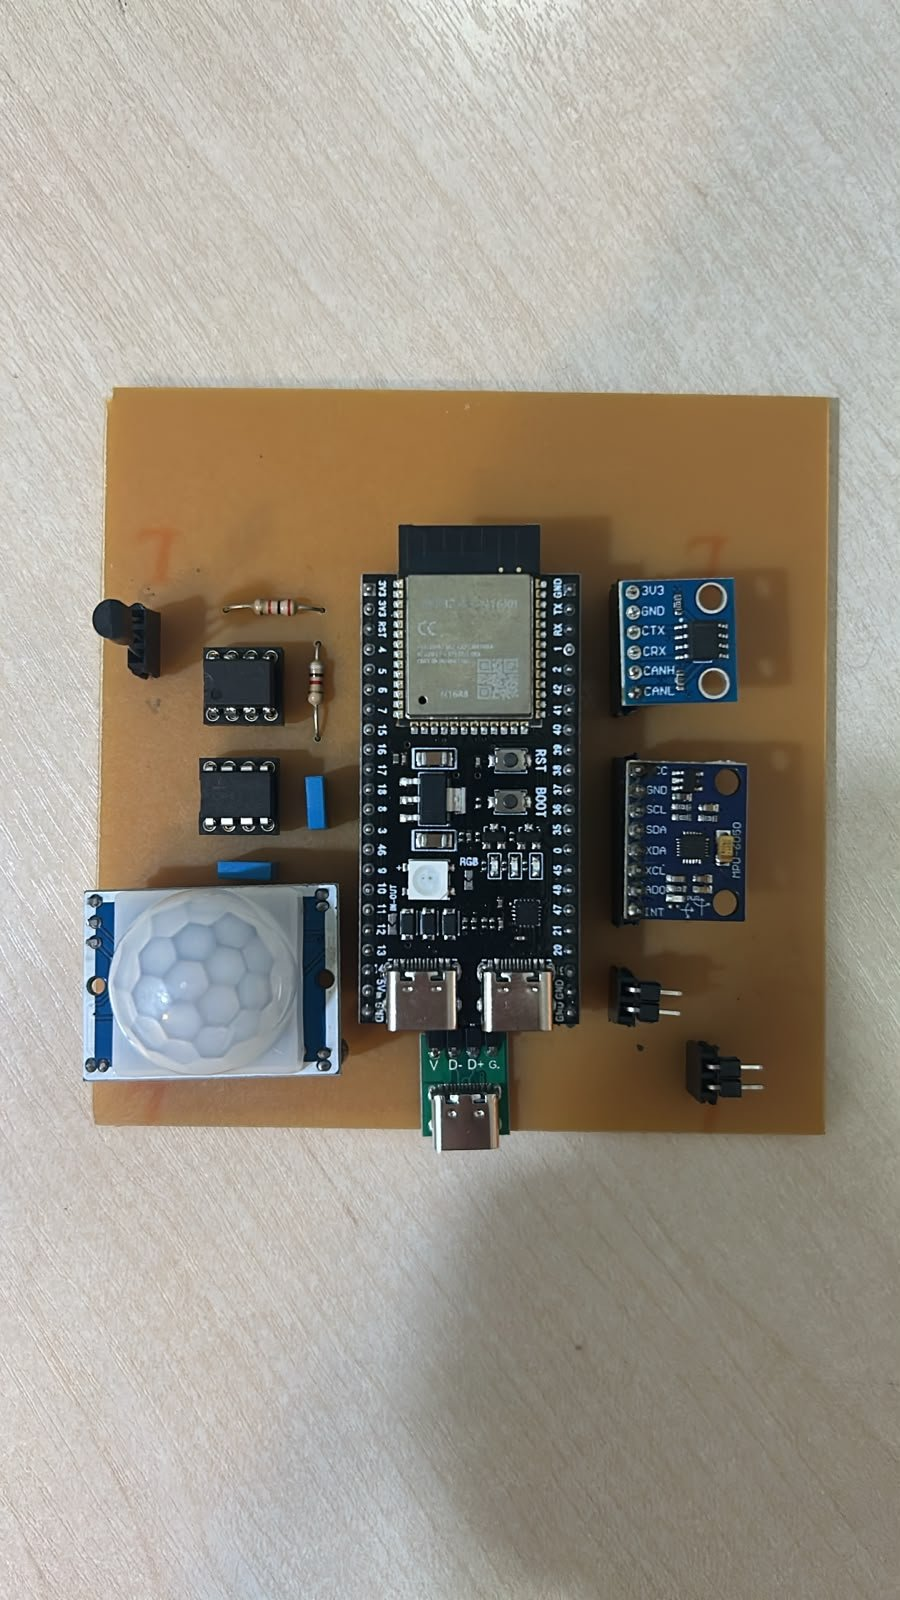
\includegraphics[height=7.5cm]{imagens/s1_pcb_montada.jpg}
\caption{A PCB de face simples do primeiro semestre, montada.}
\label{fig:pcb_s1}
\end{figure}

	%======================================================================
\section{Firmware}\label{sec:firmware}
%======================================================================
\subsection{Ambiente e organização}

O firmware das duas placas é escrito em C com o ESP-IDF 6.0.1~\cite{espidf}, que já traz o
FreeRTOS, as pilhas de Wi-Fi e TCP/IP, o cliente MQTT e os drivers dos periféricos. São dois
projetos, um por placa, e um conjunto de componentes comuns que as duas compilam
(Tabela~\ref{tab:componentes}). Cada placa passa os seus pinos e tópicos aos componentes por
uma estrutura de configuração; nada é copiado de uma placa para a outra.

\begin{table}[H]
\centering
\caption{Componentes do firmware.}
\label{tab:componentes}
\small
\begin{tabular}{@{}l>{\raggedright\arraybackslash}p{11.6cm}@{}}
\toprule
Componente & Responsabilidade \\
\midrule
\multicolumn{2}{@{}l}{\textit{Comuns (\code{firmware/common/})}} \\
\code{pcb} & mapa de pinos da PCB única, conferido na compilação \\
\code{protocol} & o contrato em C: tópicos MQTT, identificadores CAN, mensagens ESP-NOW \\
\code{rtos\_util} & prioridades nomeadas, núcleos e tamanhos de pilha das tasks \\
\code{sys\_events} & \textit{event group} com o estado do sistema: rede, hora, MQTT, CAN \\
\code{net} & Wi-Fi STA, reconexão com espera crescente, SNTP \\
\code{mqtt\_link} & cliente MQTT 3.1.1 com \textit{Last Will}, fila de saída e novas tentativas \\
\code{can} & transporte TWAI: fila de transmissão, recuperação de \textit{bus-off}, filtro e diretório de IDs \\
\code{indicators} & LED WS2812 numa task própria \\
\midrule
\multicolumn{2}{@{}l}{\textit{Hub (\code{firmware/room/})}} \\
\code{sensors} & eventos das entradas com filtro de \textit{glitch} e \textit{debounce}; drivers do PIR, das portas e do LM35 \\
\code{rules} & motor de regras em C puro, testado no computador \\
\code{hub\_config} & configuração em JSON recebida por MQTT, validada e gravada na NVS \\
\code{espnow\_link} & recepção ESP-NOW: validação, descarte de reenvios, remetente pareado \\
\midrule
\multicolumn{2}{@{}l}{\textit{Vestível (\code{firmware/gadget/})}} \\
\code{mpu6050} & driver do sensor: configuração, FIFO, detecção de sensor perdido \\
\code{fall\_pipeline} & pipeline de queda em C puro, gerado e testado contra o Python \\
\code{signal\_proc} & buffer circular, momentos com ESP-DSP e nível de atividade \\
\code{espnow\_tx} & envio ESP-NOW: varredura de canal, confirmação, reenvio \\
\code{battery} & leitura de um divisor no ADC (para uma placa futura com LiPo) \\
\bottomrule
\end{tabular}
\end{table}

A configuração de cada placa (rede, broker, chaves, MAC do par, opcionais) é feita no
\code{menuconfig} e fica no \code{sdkconfig}, que não vai para o repositório: senhas e chaves
nunca entram no git. O que vale para todos (watchdog, partições) fica num
\code{sdkconfig.defaults} versionado.

\subsection{Tasks, núcleos e recursos compartilhados}\label{sec:tasks}

As tasks seguem o padrão das aulas de RTOS~\cite{slides}: prioridades nomeadas, nunca acima de 20 (a task
do Wi-Fi roda em 23), e cada task fixada num núcleo. O núcleo 0 fica com o rádio e tudo o
que fala com ele; o núcleo 1, com o tempo real (Tabela~\ref{tab:tasks}).

\begin{table}[H]
\centering
\caption{Tasks das duas placas.}
\label{tab:tasks}
\small
\begin{tabular}{@{}llll>{\raggedright\arraybackslash}p{6.6cm}@{}}
\toprule
Placa & Task & Núcleo & Prioridade & Função \\
\midrule
hub & \code{sensors\_task} & 1 & ALTA (15) & estabiliza e lê as portas e o PIR \\
hub & \code{lm35\_task} & 1 & BAIXA (5) & temperatura a cada 30\,s \\
hub & \code{hub\_task} & 0 & MÉDIA (10) & regras, publicação, LED \\
hub & \code{espnow\_task} & 0 & MÉDIA (10) & valida e encaminha as mensagens do vestível \\
as duas & \code{can\_rx}, \code{can\_tx} & 0 & MÉDIA (10) & recepção e transmissão CAN \\
as duas & \code{indicators} & 0 & MÍNIMA (2) & LED \\
vestível & \code{sampling} & 1 & ALTA (15) & FIFO do MPU-6050 e pipeline de queda \\
vestível & \code{comm} & 0 & MÉDIA (10) & ESP-NOW, botão, heartbeat, opcionais \\
\bottomrule
\end{tabular}
\end{table}

Os recursos compartilhados seguem regras simples, que evitam corridas e travamentos:
\begin{itemize}
  \item \textbf{Filas, sempre por valor.} Quem produz um evento nunca toca o estado de quem
        consome. Interrupções e \textit{callbacks} de rádio só enfileiram ou notificam.
  \item \textbf{Event group} para o estado do sistema (rede, hora, MQTT, CAN), com um único
        escritor por bit.
  \item \textbf{Notificação de task} onde um aviso não pode se perder: o \textit{callback} de
        estado do TWAI só acorda a \code{can\_tx}, que lê o estado ela mesma.
  \item \textbf{Mutex} só para somar um lote de atividade no vestível, e seção crítica
        (\code{portMUX}) só para poucas instruções.
  \item Nenhuma task segura duas travas ao mesmo tempo, e as tasks vigiadas pelo
        \textit{watchdog} de 30\,s só esperam com tempo limite.
\end{itemize}

\subsection{Hub do quarto}

\paragraph{Fluxo.} Tudo o que acontece no quarto vira um evento na fila do hub, e uma única
task, a \code{hub\_task}, roda as regras e publica (Figura~\ref{fig:tasks_hub}). Por isso o
motor de regras não precisa de travas. As mudanças de porta e de presença e cada temperatura
saem por MQTT e pelo CAN; as mensagens do vestível chegam pela \code{espnow\_task}, que as
valida antes (versão, tipo, tamanho, remetente pareado e reenvios).

\begin{figure}[H]
\centering
\resizebox{\linewidth}{!}{% Hub: fontes de eventos -> fila do hub -> hub_task (única que roda as regras e publica).
\begin{tikzpicture}[font=\scriptsize, node distance=4mm]
  \tikzset{task/.style={bloco=#1, minimum width=2.5cm, minimum height=0.8cm},
           isr/.style={draw=black!50, fill=black!4, rounded corners=1pt, align=center, minimum width=2.1cm, minimum height=0.7cm},
           fila/.style={draw=black!60, fill=white, minimum width=0.9cm, minimum height=0.42cm, font=\tiny,
                        path picture={\foreach \k in {1,2,3} \draw[black!40] ($(path picture bounding box.west)!\k/4!(path picture bounding box.east)$) ++(0,-0.2) -- ++(0,0.4);}}}
  % fontes
  \node[isr] (isr) at (0,3.0) {ISR do GPIO\\(portas, PIR)};
  \node[task=corhub] (sens) at (4.0,3.0) {\textbf{sensors\_task}\\núcleo 1, ALTA};
  \node[task=corhub] (lm) at (4.0,1.8) {\textbf{lm35\_task}\\núcleo 1, BAIXA};
  \node[task=corambas] (esp) at (4.0,0.6) {\textbf{espnow\_task}\\núcleo 0, MÉDIA};
  \node[isr] (espcb) at (-0.2,0.6) {callback de\\recepção ESP-NOW};
  \node[isr] (mq) at (4.0,-0.6) {MQTT\\\code{config/desejada}};
  \node[fila] (q1) at (1.95,3.0) {};
  \node[fila] (q0) at (1.95,0.6) {};
  \draw[seta] (isr) -- (q1); \draw[seta] (q1) -- (sens);
  \draw[seta] (espcb) -- (q0); \draw[seta] (q0) -- (esp);
  % fila do hub e hub_task
  \node[fila, minimum width=1.4cm, minimum height=0.55cm] (qh) at (6.9,1.2) {};
  \node[font=\tiny, above=0pt of qh] {fila do hub};
  \node[task=corhub, minimum width=2.8cm, minimum height=1.2cm] (hub) at (9.5,1.2) {\textbf{hub\_task}\\núcleo 0, MÉDIA\\regras + publicação};
  \foreach \n in {sens,lm,esp,mq} {\draw[seta] (\n.east) -- ++(0.3,0) |- (qh.west);}
  \draw[seta] (qh) -- (hub);
  % saídas
  \node[bloco=corcentral, minimum width=2.2cm] (mqtt) at (13.0,2.6) {MQTT\\(estados, alertas)};
  \node[bloco=cinza, minimum width=2.2cm] (led) at (13.0,1.2) {LED\\(\code{indicators})};
  \node[fila] (qc) at (12.0,-0.2) {};
  \node[task=corambas, minimum width=2.1cm] (ctx) at (13.8,-0.2) {\textbf{can\_tx}\\TWAI};
  \draw[seta] (hub.east) -- ++(0.3,0) |- (mqtt.west);
  \draw[seta] (hub.east) -- (led.west);
  \draw[seta] (hub.east) -- ++(0.3,0) |- (qc.west);
  \draw[seta] (qc) -- (ctx);
  % recepção CAN
  \node[isr] (twai) at (6.9,-1.6) {ISR do TWAI};
  \node[fila] (qr) at (8.9,-1.6) {};
  \node[task=corambas, minimum width=2.1cm] (crx) at (10.9,-1.6) {\textbf{can\_rx}\\log};
  \draw[seta] (twai) -- (qr); \draw[seta] (qr) -- (crx);
  % legenda
  \node[fila, anchor=west] (lf) at (0,-1.6) {};
  \node[anchor=west, font=\tiny] at (lf.east) {fila (por valor)};
\end{tikzpicture}
}
\caption{Tasks e filas do hub. A \code{hub\_task} é a única que chama as regras e publica.}
\label{fig:tasks_hub}
\end{figure}

\paragraph{Regras.}\label{sec:regras} O motor de regras (Tabela~\ref{tab:regras}) é C puro,
sem dependência do ESP-IDF, e roda também no computador, onde é testado. Cada alerta é um
\textbf{episódio}: publicado uma vez como \code{ativo} e encerrado como \code{resolvido} ou
\code{cancelado}, sem repetição (Figura~\ref{fig:alerta_estados}). Sem hora válida, as regras
com janela de horário ficam suspensas, e o \code{status} do hub informa
\code{"hora":false}. A inatividade só vale de dia porque, à noite, o residente dormindo não
aciona o PIR.

\begin{table}[H]
\centering
\caption{Regras de alerta do hub (valores padrão, ajustáveis por MQTT).}
\label{tab:regras}
\small
\begin{tabular}{@{}l>{\raggedright\arraybackslash}p{4.9cm}>{\raggedright\arraybackslash}p{3.8cm}>{\raggedright\arraybackslash}p{1.9cm}@{}}
\toprule
Tipo & Dispara quando & Resolve quando & Padrão \\
\midrule
\code{queda} & chega uma \code{FALL} do vestível & ``estou bem'' (\code{cancelado}) & --- \\
\code{saida\_noturna} & a porta de saída abre à noite e passam N\,min sem presença & a presença volta & 22h--6h, 15\,min \\
\code{banheiro\_prolongado} & a porta do banheiro fecha e passam N\,min sem presença e sem a saída abrir & a porta do banheiro abre & 40\,min \\
\code{inatividade} & de dia, N\,min sem presença e sem a saída abrir & a presença volta & 120\,min \\
\code{temperatura} & fora da faixa por 10\,min seguidos & dentro da faixa (histerese de 0,5\,°C) por 10\,min & 18--28\,°C \\
\code{vestivel\_offline} & 90\,s sem mensagens do vestível & a próxima mensagem & --- \\
\code{bateria\_baixa} & bateria do vestível abaixo do limite & acima de 3,6\,V & 3,5\,V \\
\bottomrule
\end{tabular}
\end{table}

\begin{figure}[H]
\centering
\resizebox{0.9\linewidth}{!}{% Ciclo de vida de um episódio de alerta no hub.
\begin{tikzpicture}[font=\scriptsize, >=Stealth]
  \tikzset{estado/.style={draw=#1, fill=#1!10, thick, rounded corners=8pt, minimum width=2.2cm, minimum height=0.9cm, align=center}}
  \node[estado=cinza] (ok) at (0,0) {normal\\(sem episódio)};
  \node[estado=corvest] (at) at (5.0,0) {\textbf{ativo}\\LED vermelho};
  \node[estado=corcentral] (res) at (10.6,1.4) {\textbf{resolvido}};
  \node[estado=corcentral] (can) at (10.6,-1.4) {\textbf{cancelado}};
  \draw[->, thick] (ok) -- node[rotulo, above=2pt] {condição da regra} node[rotulo, below=2pt] {publica \code{ativo}} (at);
  \draw[->, thick] (at.east) ++(0,0.2) -- node[rotulo, above=3pt, sloped] {a condição acabou} (res.west);
  \draw[->, thick] (at.east) ++(0,-0.2) -- node[rotulo, below=3pt, sloped] {``estou bem'' (só queda)} (can.west);
  \draw[->, thick, black!50] (res.north) to[out=150, in=40] node[rotulo, above] {publica \code{resolvido} e volta ao normal} (ok.north);
  \draw[->, thick, black!50] (can.south) to[out=210, in=-40] node[rotulo, below] {publica \code{cancelado} e volta ao normal} (ok.south);
\end{tikzpicture}
}
\caption{Ciclo de vida de um episódio de alerta.}
\label{fig:alerta_estados}
\end{figure}

\paragraph{Configuração sem recompilar.} Os parâmetros das regras chegam pelo tópico
\code{config/desejada}, em JSON. O hub valida tudo, grava na NVS e responde em
\code{config/aplicada}; uma configuração inválida é recusada inteira, e a anterior continua
valendo. No boot, o hub usa a NVS ou, se ela estiver vazia, os valores padrão:
\begin{lstlisting}[language=json]
{"v":1, "noite":{"inicio":"22:00","fim":"06:00"},
 "portas":{"quarto":"saida","banheiro":"banheiro"},
 "saida_noturna_min":15, "banheiro_min":40, "inatividade_min":120,
 "temperatura":{"min":18,"max":28,"histerese":0.5,"persistencia_min":10},
 "vestivel_offline_s":90, "bateria_baixa_mV":3500}
\end{lstlisting}

\subsection{Vestível}

\paragraph{Aquisição.} A task \code{sampling} lê a FIFO do MPU-6050 a cada 50\,ms e passa
cada amostra pelo pipeline de queda (Figura~\ref{fig:tasks_vestivel};
Seção~\ref{sec:queda}). Se a FIFO transbordar ou a leitura falhar no meio, a FIFO é zerada e
o pipeline recomeça: uma janela nunca junta trechos dos dois lados de uma lacuna. Dez leituras
seguidas sem amostra (0,5\,s) significam que o sensor parou (um MPU que reinicia volta
dormindo); o vestível passa então a procurar o sensor a cada 5\,s.

\begin{figure}[H]
\centering
\resizebox{\linewidth}{!}{% Vestível: sampling (núcleo 1) roda o pipeline; comm (núcleo 0) cuida do rádio.
\begin{tikzpicture}[font=\scriptsize]
  \tikzset{etapa/.style={draw=corvest, fill=corvest!8, rounded corners=2pt, align=center, minimum height=0.8cm,
                         minimum width=1.55cm, inner sep=2pt},
           fila/.style={draw=black!60, fill=white, minimum width=0.9cm, minimum height=0.42cm, font=\tiny,
                        path picture={\foreach \k in {1,2,3} \draw[black!40] ($(path picture bounding box.west)!\k/4!(path picture bounding box.east)$) ++(0,-0.2) -- ++(0,0.4);}}}
  \node[draw=black!50, fill=black!4, rounded corners=1pt, align=center, minimum height=0.8cm] (mpu) at (-0.7,0)
       {MPU-6050\\FIFO (200\,Hz)};
  \node[etapa] (f) at (2.4,0) {passa-baixa\\20\,Hz (6 eixos)};
  \node[etapa] (g) at (4.4,0) {gatilho\\$\amag \ge 2$\,g};
  \node[etapa] (j) at (6.4,0) {janela\\$-$1,0 a +0,8\,s};
  \node[etapa] (a) at (8.4,0) {23\\atributos};
  \node[etapa] (c) at (10.4,0) {Random\\Forest};
  \node[etapa] (d) at (12.4,0) {$P \ge$ limiar?\\cooldown 30\,s};
  \draw[seta] (mpu) -- node[rotulo, below=9pt] {I²C, a cada 50\,ms} (f);
  \foreach \u/\v in {f/g, g/j, j/a, a/c, c/d} {\draw[seta] (\u) -- (\v);}
  \begin{scope}[on background layer]
    \node[draw=corvest, dashed, rounded corners, fit=(f)(d), inner sep=3mm,
          label={[font=\scriptsize\bfseries, text=corvest]above:\textbf{sampling}: núcleo 1, prioridade ALTA}] (samp) {};
  \end{scope}
  % comm
  \node[fila] (q) at (12.4,-1.9) {};
  \node[bloco=corvest, minimum width=3.0cm] (comm) at (9.4,-1.9) {\textbf{comm}: núcleo 0, MÉDIA\\ESP-NOW, heartbeat, botão};
  \draw[seta] (d) -- node[rotulo, right] {queda} (q);
  \draw[seta] (q) -- (comm);
  \node[draw=black!50, fill=black!4, rounded corners=1pt, align=center] (bt) at (5.6,-1.9) {botão\\(ISR)};
  \draw[seta] (bt) -- (comm);
  \node[bloco=corhub, minimum width=2.2cm] (hub) at (9.4,-3.5) {hub\\(ESP-NOW cifrado)};
  \draw[sem fio=corvest] (comm) -- node[rotulo, right] {\code{FALL}, \code{FALL\_CANCEL}, \code{HEARTBEAT}} (hub);
  \node[draw=black!40, dashed, rounded corners, align=center, font=\tiny] (op) at (5.6,-3.5)
       {opcionais: MQTT direto\\e CAN de bancada};
  \draw[seta=black!40, dashed] (comm.west) ++(0,-0.3) -| (op.north);
\end{tikzpicture}
}
\caption{O vestível: a task \code{sampling} roda o pipeline amostra a amostra no núcleo 1, e a
\code{comm} cuida do rádio no núcleo 0.}
\label{fig:tasks_vestivel}
\end{figure}

\paragraph{Comunicação e interação.} A \code{comm} manda a \code{FALL} na hora em que o
pipeline decide queda, e o LED fica em alerta durante a janela de cancelamento de 15\,s; se o
botão for apertado nesse tempo, sai uma \code{FALL\_CANCEL}. A cada 30\,s sai um
\code{HEARTBEAT} com a bateria e o nível de atividade, o valor RMS de $\amag - 1$\,g desde o
heartbeat anterior. Os detalhes do enlace estão na Seção~\ref{sec:espnow}.

\paragraph{Modos.}
\begin{itemize}
  \item \textbf{Normal}: ESP-NOW até o hub.
  \item \textbf{Coleta}: cada amostra bruta e cada janela classificada (com os 23 atributos e
        a probabilidade) vão para a serial. É assim que vai ser formado o conjunto de dados
        no pulso (Seção~\ref{sec:queda}).
  \item \textbf{Sem hub}: com o MAC do hub vazio na configuração, o ESP-NOW não é ligado e as
        quedas vão só para o log. É o modo de bancada e de demonstração com uma placa só,
        ligada ao computador pela USB (Seção~\ref{sec:demo}).
  \item \textbf{Opcionais}, desligados por padrão: MQTT direto ao broker, como reserva se o
        hub não confirmar uma queda, e CAN de bancada.
\end{itemize}

\subsection{Robustez}\label{sec:ausente}

Uma regra vale para as duas placas: \textbf{uma peça ausente gera um aviso, não um erro}.
Sensor, CAN, Wi-Fi ou broker que faltam dão um único aviso no log quando a falta é percebida e
uma informação quando voltam; as novas tentativas ficam em silêncio, com espera crescente até
60\,s. Nada opcional pode derrubar a placa:
\begin{itemize}
  \item \textbf{Vestível sem MPU-6050}: segue rodando, com o LED vermelho lento, e \textbf{não
        manda heartbeat}, para não parecer saudável sem detectar quedas; o hub o declara
        offline em 90\,s.
  \item \textbf{Hub com sensor não instalado}: um PIR solto lê ``ninguém'' e uma porta solta
        lê ``aberta'', e nada no sinal os distingue de um caso real. Por isso os sensores
        instalados são declarados no \code{menuconfig}. Sem PIR, a inatividade e a saída
        noturna ficam suspensas; uma porta ausente não é lida.
  \item \textbf{Rede}: o Wi-Fi reconecta com espera de 1 a 60\,s; o cliente MQTT só inicia
        com a rede de pé e é reiniciado se o início falhar.
  \item \textbf{Queda que não chegou}: a \code{FALL} é guardada e reenviada igual até ser
        entregue (Seção~\ref{sec:espnow}).
  \item \textbf{Configuração errada não compila}: pino repetido ou proibido, chave do ESP-NOW
        com tamanho diferente de 16 caracteres ou MAC mal escrito fazem o build falhar, com a
        mensagem do problema.
\end{itemize}

\subsection{Testes no computador}

A lógica que não depende de hardware é C puro e roda também no computador, compilada com o
gcc. Cada componente tem uma bateria de testes (Tabela~\ref{tab:testes}); os do pipeline de
queda comparam o C, janela a janela, com o Python que treinou o modelo.

\begin{table}[H]
\centering
\caption{Testes automáticos que rodam no computador (sem placa).}
\label{tab:testes}
\small
\begin{tabular}{@{}l>{\raggedright\arraybackslash}p{8.8cm}r@{}}
\toprule
Componente & O que verifica & Verificações \\
\midrule
\code{rules} (hub) & cada regra dispara e resolve como especificado, episódios sem repetição, queda depois de o vestível reiniciar, sensores ausentes & 62 \\
\code{hub\_config} (hub) & validação do JSON da configuração, recusa de valores inválidos & 60 \\
\code{fall\_pipeline} (vestível) & filtro, gatilho e, em 26 janelas de 8 trechos da SisFall, os mesmos picos, atributos e probabilidades do Python & 885 \\
\code{signal\_proc} (vestível) & buffer circular, atributos, nível de atividade & 25 \\
\midrule
notificador (central) & formatação, reenvio ao Telegram, dados inesperados & 19 testes \\
\code{demo\_vestivel.py} & leitura da serial, reconexão, linhas estragadas & 15 testes \\
\code{modelo/} (Python) & blocos do pipeline contra os exemplos das aulas, leitura dos dados & 30 testes \\
\bottomrule
\end{tabular}
\end{table}

\subsection{Uso de memória}

A Tabela~\ref{tab:memoria} mostra o tamanho de cada firmware, medido pelo \code{idf.py size}.
A partição de aplicação tem 1,5\,MB. A maior parte da imagem é a pilha de Wi-Fi, TCP/IP e TLS;
a floresta do modelo de queda ocupa \rfKB\,kB.

\begin{table}[H]
\centering
\caption{Uso de memória (ESP-IDF 6.0.1, \code{idf.py size}).}
\label{tab:memoria}
\small
\begin{tabular}{@{}lrrr@{}}
\toprule
Firmware & Imagem (bytes) & Partição livre & RAM interna usada \\
\midrule
Hub & 992\,672 & 35\,\% & 112\,135 B (32,8\,\%) \\
Vestível com ESP-NOW & 960\,688 & 37\,\% & 130\,615 B (38,2\,\%) \\
Vestível sem hub (bancada) & 383\,184 & 75\,\% & 86\,203 B (25,2\,\%) \\
\bottomrule
\end{tabular}
\end{table}

	%======================================================================
\section{Interface com a rede CAN}\label{sec:can}
%======================================================================
\subsection{O barramento da sala}

A disciplina pede que os módulos de todos os grupos da sala conversem por um barramento CAN.
No nosso sistema, o CAN não é o caminho até a central (isso é o MQTT): ele integra o hub aos
módulos dos outros grupos e publica nele os estados dos sensores do quarto. O vestível também
tem CAN, mas só para bancada e testes; a pulseira de verdade não tem transceptor.

O CAN foi escolhido no primeiro semestre no lugar do RS-485 com Modbus por três motivos que
continuam valendo: o barramento é multimestre, sem um nó que precise perguntar a cada um; a
arbitragem por identificador resolve colisões sem perder a mensagem mais prioritária; e o
controlador do próprio ESP32-S3 faz o enquadramento, o CRC, a confirmação e a retransmissão
em hardware, como define a norma~\cite{iso11898}.

\subsection{Camada física e controlador}

\begin{table}[H]
\centering
\caption{Parâmetros do barramento CAN.}
\label{tab:can_param}
\small
\begin{tabular}{@{}>{\raggedright\arraybackslash}p{3.6cm}>{\raggedright\arraybackslash}p{10.2cm}@{}}
\toprule
Item & Valor \\
\midrule
Controlador & TWAI do ESP32-S3 (compatível com CAN 2.0), TX no GPIO 13 e RX no GPIO 14, nas duas placas \\
Transceptor & SN65HVD230~\cite{sn65hvd230}, de 3,3\,V, no módulo WCMCU-230 (J1), com o barramento em J7 (CANH, CANL, GND) \\
Taxa & 250\,kbit/s \\
Quadro & CAN clássico, identificador padrão de 11 bits, até 8 bytes de dados \\
Terminação & 120\,$\Omega$ nas duas pontas do barramento \\
Filtro de aceitação & em hardware: só os IDs de \code{0x000} a \code{0x0FF} chegam ao firmware \\
Erros & retransmissão até haver confirmação; em \textit{bus-off}, nova tentativa de recuperação com espera de 1 a 60\,s \\
Modo de bancada & autoconfirmação com \textit{loopback} interno, ligado por padrão: testa o firmware sem barramento. Desligado no barramento real \\
\bottomrule
\end{tabular}
\end{table}

O transceptor é de 3,3\,V, o mesmo nível dos GPIOs, e é alimentado pelo regulador da
DevKit; o SN65HVD230 gera os níveis diferenciais do barramento a partir dele. Os pontos de
teste TP5 e TP6, em CANH e CANL, permitem olhar o barramento com o osciloscópio.

\subsection{Identificadores e mensagens}

Toda a identidade de uma mensagem está no identificador, no formato \code{0x0GS}
(Figura~\ref{fig:can_id}): \code{G} é o grupo da sala e \code{S} o sensor dentro do grupo.
Os 8 bytes de dados ficam só para o valor. Esse formato foi combinado entre os grupos: cada
um tem 16 identificadores próprios, e o filtro de hardware descarta o resto. Como no CAN o
menor ID ganha a arbitragem, a prioridade entre os grupos fica definida pelo nibble do grupo.

\begin{figure}[H]
\centering
\resizebox{\linewidth}{!}{% Quadro CAN clássico com ID de 11 bits e o formato 0x0GS do identificador.
\begin{tikzpicture}[font=\scriptsize]
  \tikzset{campo/.style={draw=black!60, fill=#1, minimum height=0.7cm, align=center, inner sep=1pt},
           campo/.default=white}
  % quadro
  \def\y{0}
  \node[campo=black!8, minimum width=0.7cm, anchor=west] (sof) at (0,\y) {SOF\\1};
  \node[campo=corambas!20, minimum width=3.3cm, anchor=west] (id) at (sof.east) {identificador\\11 bits};
  \node[campo=black!8, minimum width=0.7cm, anchor=west] (rtr) at (id.east) {RTR\\1};
  \node[campo=black!8, minimum width=1.0cm, anchor=west] (ide) at (rtr.east) {IDE, r0\\2};
  \node[campo=black!8, minimum width=0.9cm, anchor=west] (dlc) at (ide.east) {DLC\\4};
  \node[campo=corhub!15, minimum width=3.0cm, anchor=west] (dados) at (dlc.east) {dados\\0 a 8 bytes};
  \node[campo=black!8, minimum width=1.2cm, anchor=west] (crc) at (dados.east) {CRC\\15 + 1};
  \node[campo=black!8, minimum width=0.9cm, anchor=west] (ack) at (crc.east) {ACK\\2};
  \node[campo=black!8, minimum width=0.9cm, anchor=west] (eof) at (ack.east) {EOF\\7};
  % zoom do identificador
  \foreach \b [count=\i from 0] in {10,9,8,7,6,5,4,3,2,1,0} {
    \pgfmathsetmacro{\x}{1.0 + \i*0.85}
    \ifnum\b>7 \def\cor{black!8}\else\ifnum\b>3 \def\cor{corambas!30}\else\def\cor{corhub!25}\fi\fi
    \node[campo=\cor, minimum width=0.85cm, minimum height=0.6cm] (b\b) at (\x,-2.0) {\b};
  }
  \draw[decorate, decoration={brace, amplitude=4pt, mirror}] (b10.south west) -- (b8.south east)
       node[midway, below=5pt, align=center] {0\\(ID $\le$ \code{0x0FF})};
  \draw[decorate, decoration={brace, amplitude=4pt, mirror}] (b7.south west) -- (b4.south east)
       node[midway, below=5pt, align=center] {\textbf{G}: grupo\\(\code{0xF} = este projeto)};
  \draw[decorate, decoration={brace, amplitude=4pt, mirror}] (b3.south west) -- (b0.south east)
       node[midway, below=5pt, align=center] {\textbf{S}: sensor\\dentro do grupo};
  \draw[black!40, dashed] (id.south west) -- (b10.north west);
  \draw[black!40, dashed] (id.south east) -- (b0.north east);
  \node[anchor=west, align=left] at (10.6,-2.0) {ex.: \code{0x0F2}\\= grupo F,\\sensor 2 (LM35)};
\end{tikzpicture}
}
\caption{Quadro CAN clássico (campos e número de bits) e o identificador no formato
\code{0x0GS}.}
\label{fig:can_id}
\end{figure}

\begin{table}[H]
\centering
\caption{Mensagens CAN deste projeto (grupo \code{0xF}). Valores em \textit{little endian}.}
\label{tab:can_msgs}
\small
\begin{tabular}{@{}l>{\raggedright\arraybackslash}p{2.1cm}>{\raggedright\arraybackslash}p{2.3cm}>{\raggedright\arraybackslash}p{7.4cm}@{}}
\toprule
ID & Placa & Sensor & Dados \\
\midrule
\code{0x0F1} & hub & HC-SR501 & 1 byte: 0 = livre, 1 = presença \\
\code{0x0F2} & hub & LM35 & 2 bytes: \code{int16} em centésimos de °C \\
\code{0x0F3}--\code{0x0FA} & hub & portas (até 8) & 1 byte: 0 = fechada, 1 = aberta. \code{0x0F3} = quarto, \code{0x0F4} = banheiro \\
\code{0x0FD} & vestível (bancada) & MPU-6050 & 3 bytes: \code{int16} com $\amag^2$ no pico em centésimos de g$^2$ e \code{uint8} com P(queda) em \% \\
\code{0x0FE} & vestível (bancada) & --- & 4 bytes: \code{uint16} bateria em mV (\code{0xFFFF} = não medida) e \code{uint16} atividade em mg \\
\bottomrule
\end{tabular}
\end{table}

O hub envia um quadro a cada mudança de porta ou de presença e a cada leitura de temperatura
(30\,s). Os quadros dos outros grupos e os do vestível em bancada vão para o log do hub; eles
ainda não têm tópico MQTT. Os quadros do vestível não entram nas regras: o alerta de queda
depende do número de sequência do ESP-NOW (Seção~\ref{sec:espnow}).

\paragraph{Carga do barramento.} Um quadro com 1 ou 2 bytes de dados tem cerca de 65 a 75 bits,
contando o enchimento de bits; a 250\,kbit/s, ocupa o barramento por $\sim$0,3\,ms. Mesmo com
as portas e a presença mudando várias vezes por minuto, o hub usa uma fração desprezível do
barramento, que fica para os outros grupos.

\subsection{Implementação}

O componente \code{can} é o mesmo nas duas placas. Qualquer task chama
\code{can\_transmit()}, que só enfileira o quadro; só a task \code{can\_tx} toca o driver.
Assim, nenhuma task espera o barramento, e um barramento sem ninguém (sem confirmação) não
trava quem publica. O estado do nó é acompanhado pela \code{can\_tx}, avisada por notificação:
\begin{itemize}
  \item em \textit{bus-off} (excesso de erros de transmissão), o nó se desliga do barramento,
        como manda o protocolo. O firmware dá \textbf{um} aviso (``CAN sem barramento'') e tenta
        recuperar com espera crescente, de 1 a 60\,s, para não encher o log nem o barramento
        quando ele simplesmente não existe (placa sem transceptor);
  \item só depois que um quadro sai de fato (contador de erros de transmissão zerado) o
        firmware considera o barramento de volta, e avisa uma vez;
  \item quadros que não saem a tempo são descartados, com uma contagem no log.
\end{itemize}

A recepção usa a interrupção do TWAI, que só põe o quadro numa fila; a task \code{can\_rx}
decodifica pelo diretório de identificadores e registra no log. Quadros remotos (RTR) são
ignorados.

\subsection{Validação}

O CAN foi validado com o professor em 28/08/2026, no Projeto 1 deste semestre, com o
firmware de então e os módulos dos outros grupos (Figura~\ref{fig:can_s2p1}). O transporte
foi reescrito depois (filas, recuperação de \textit{bus-off}, diretório de IDs, mapa de pinos
novo), e a versão atual foi verificada em build e no modo de bancada; o teste entre as duas
placas montadas, com transceptores e terminação, está no plano da
Seção~\ref{sec:verificacao}.

\begin{figure}[H]
\centering
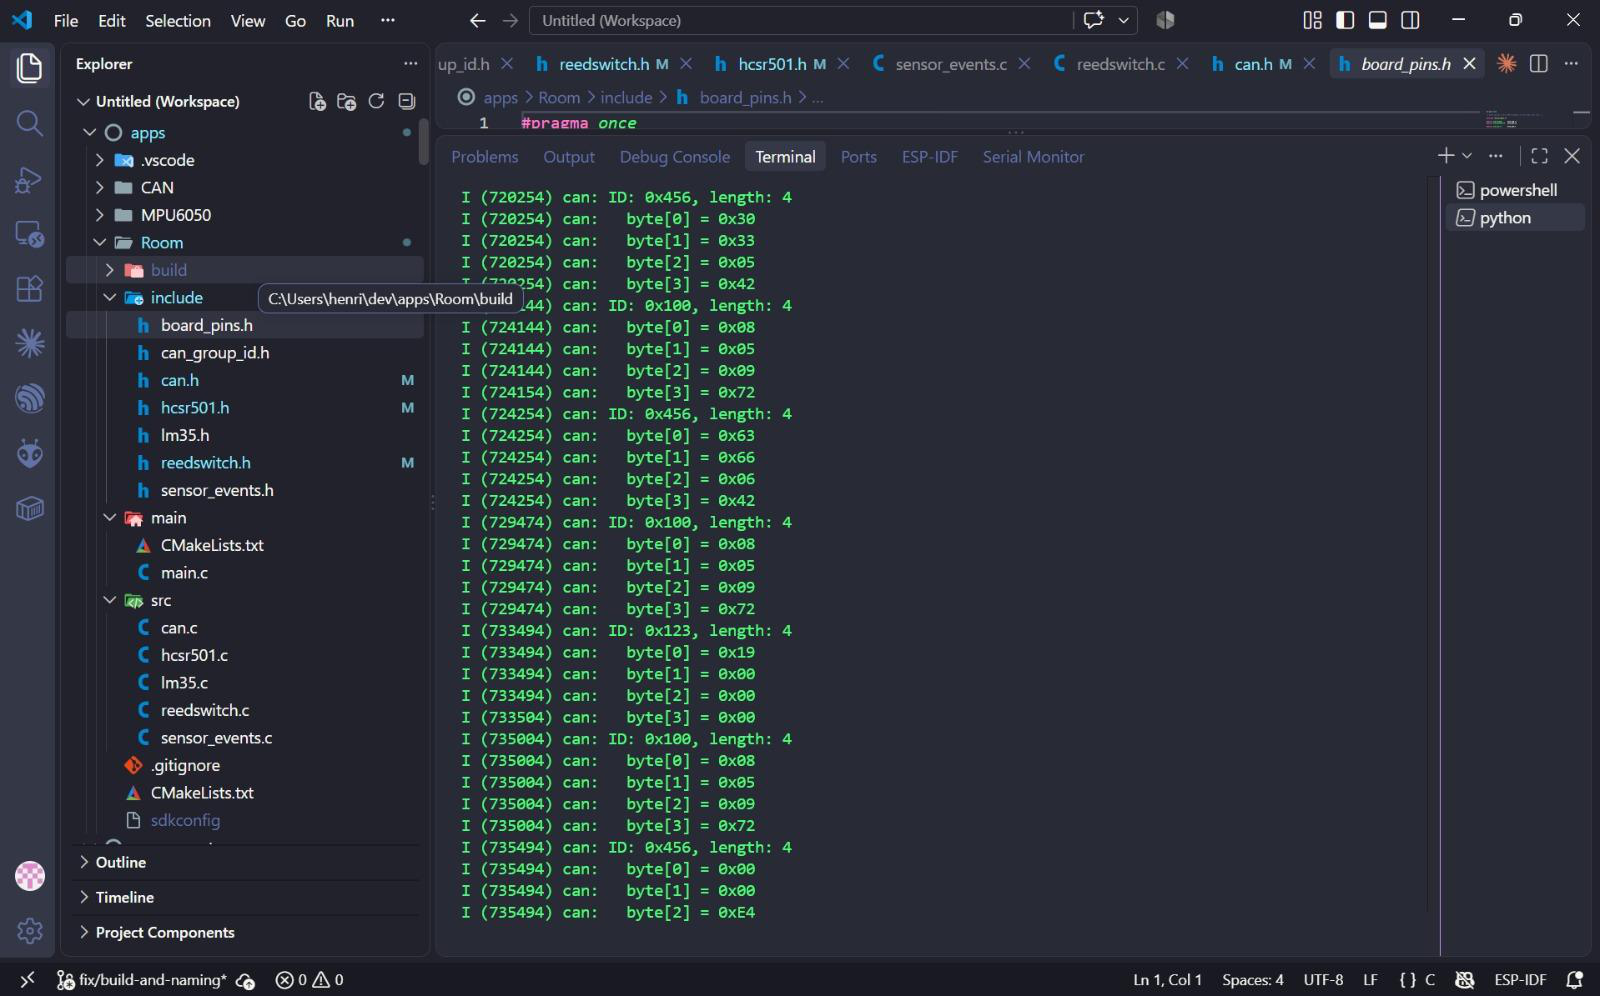
\includegraphics[width=0.85\linewidth]{imagens/s2p1_can_serial.png}
\caption{Monitor serial na validação de 28/08/2026: quadros recebidos do barramento da
sala, com o identificador, o tamanho e os bytes.}
\label{fig:can_s2p1}
\end{figure}

\begin{figure}[H]
\centering
\begin{subfigure}[b]{0.49\linewidth}
  \centering
  \fotoouespaco{bancada_can}{\linewidth}{as duas placas ligadas pelo barramento CAN (transceptores e terminação)}
\end{subfigure}\hfill
\begin{subfigure}[b]{0.49\linewidth}
  \centering
  \fotoouespaco{serial_can}{\linewidth}{monitor serial do hub com os quadros 0x0FD/0x0FE do vestível}
\end{subfigure}
\caption{Teste do CAN entre as duas placas v1.}
\label{fig:bancada_can}
\end{figure}

	%======================================================================
\section{Interface sem fio}\label{sec:semfio}
%======================================================================
O sistema tem dois enlaces sem fio, os dois em 2,4\,GHz no rádio do próprio ESP32-S3: o
\textbf{ESP-NOW}, da pulseira ao hub, e o \textbf{Wi-Fi}, do hub ao ponto de acesso da
ILPI, por onde passa o MQTT até a central.

\subsection{Modos do ESP32-S3 e o papel de cada nó}\label{sec:modos}

O rádio do ESP32-S3 pode operar como estação (STA, associada a um ponto de acesso), como
ponto de acesso (SoftAP), nos dois ao mesmo tempo (AP+STA) e com o ESP-NOW, um protocolo da
Espressif que troca quadros curtos direto entre dispositivos, na camada de enlace, sem
associação~\cite{espnow}. O ESP-NOW funciona sobre a interface STA ou SoftAP, no canal em que
o rádio estiver.

\begin{table}[H]
\centering
\caption{Modos do rádio em cada nó.}
\label{tab:modos}
\small
\begin{tabular}{@{}l>{\raggedright\arraybackslash}p{4.0cm}>{\raggedright\arraybackslash}p{7.8cm}@{}}
\toprule
Nó & Modo & Por quê \\
\midrule
Hub & STA associado ao Wi-Fi da ILPI, sem economia de energia, + ESP-NOW & precisa do Wi-Fi para o MQTT; sem economia de energia, porque com ela o rádio dorme entre os \textit{beacons} e perde quadros ESP-NOW \\
Pulseira & STA sem associação, só ESP-NOW & o rádio só liga para enviar; não precisa manter a associação nem conhecer a senha da rede \\
Central & --- (rede local, cabo ou Wi-Fi) & --- \\
\bottomrule
\end{tabular}
\end{table}

A primeira proposta, no Projeto 1 deste semestre, já usava o ESP-NOW, mas punha o hub em
AP+STA, com o ESP-NOW num canal fixo, sem criptografia e com mensagens em texto. Ela foi
revista: o ESP-NOW funciona sobre a interface STA, então o SoftAP não acrescentava nada; e o
que evita perder quadros no hub é desligar a economia de energia do rádio. O canal passou a
ser descoberto pela pulseira, e as mensagens ganharam formato binário e criptografia.

\subsection{ESP-NOW: da pulseira ao hub}\label{sec:espnow}

\begin{table}[H]
\centering
\caption{O enlace ESP-NOW.}
\label{tab:espnow}
\small
\begin{tabular}{@{}>{\raggedright\arraybackslash}p{3.0cm}>{\raggedright\arraybackslash}p{10.8cm}@{}}
\toprule
Item & Valor \\
\midrule
Sentido & pulseira envia, hub recebe; sempre \textit{unicast} \\
Endereçamento & o MAC do hub, configurado na pulseira; o hub aceita só a pulseira pareada \\
Criptografia & ligada: chave primária (PMK) comum e chave local (LMK) do par, 16 bytes cada, fora do repositório \\
Canal & o do Wi-Fi do hub, descoberto pela pulseira por varredura \\
Tamanho & até 13 bytes por mensagem (o limite do ESP-NOW é 250) \\
Confirmação & ACK da camada MAC do hub, informado pelo \textit{callback} de envio \\
\bottomrule
\end{tabular}
\end{table}

\paragraph{Formato.} As mensagens são estruturas empacotadas, em \textit{little endian},
definidas num cabeçalho C (\code{protocol\_espnow.h}) que as duas placas compilam
(Figura~\ref{fig:espnow_quadro}). O cabeçalho comum traz a versão do formato, o tipo, um
número de sequência e o tempo desde o boot da pulseira. São seis tipos: \code{PING} (varredura
de canal), \code{HEARTBEAT}, \code{FALL} e \code{HELP} (o pedido de ajuda, só o cabeçalho), e
os cancelamentos \code{FALL\_CANCEL} e \code{HELP\_CANCEL}, que levam a sequência do alerta
cancelado. O hub descarta versão ou tipo desconhecidos e mensagens com tamanho diferente do
esperado para o tipo.

\begin{figure}[H]
\centering
\resizebox{0.95\linewidth}{!}{% Mensagens ESP-NOW: cabeçalho de 8 bytes e o payload de cada tipo (bytes).
\begin{tikzpicture}[font=\scriptsize]
  \tikzset{byte/.style={draw=black!60, fill=#1, minimum height=0.62cm, align=center, inner sep=1pt, anchor=west},
           byte/.default=white}
  \def\u{0.62}
  % cabeçalho comum
  \foreach \y/\nome/\tam in {0/FALL/13, -1.0/HEARTBEAT/12, -2.0/FALL\_CANCEL \textrm{e} HELP\_CANCEL/10, -3.0/PING \textrm{e} HELP/8} {
    \node[anchor=east, font=\scriptsize] at (-0.15,\y) {\code{\nome} (\tam\,B)};
    \node[byte=black!8, minimum width=\u cm] (v) at (0,\y) {ver.};
    \node[byte=black!8, minimum width=\u cm] (t) at (v.east) {tipo};
    \node[byte=corhub!18, minimum width=2*\u cm] (s) at (t.east) {\code{seq}};
    \node[byte=corhub!18, minimum width=4*\u cm] (u) at (s.east) {\code{uptime\_ms}};
  }
  % payloads
  \node[byte=corvest!22, minimum width=4*\u cm] (a2) at ($(0,0)+(8*\u,0)$) {\code{a2\_peak} (float, g$^2$)};
  \node[byte=corvest!22, minimum width=\u cm*1.6] at (a2.east) {\code{prob}\\\%};
  \node[byte=corcentral!22, minimum width=2*\u cm] (bat) at ($(0,-1.0)+(8*\u,0)$) {bateria (mV)};
  \node[byte=corcentral!22, minimum width=2*\u cm] at (bat.east) {atividade (mg)};
  \node[byte=corvest!22, minimum width=2*\u cm] at ($(0,-2.0)+(8*\u,0)$) {\code{seq} do\\[-2pt]alerta};
  % réguas
  \draw[decorate, decoration={brace, amplitude=4pt}] (0,0.42) -- (8*\u,0.42) node[midway, above=5pt] {cabeçalho comum: 8 bytes};
  \draw[decorate, decoration={brace, amplitude=4pt}] (8*\u,0.42) -- (13*\u+0.6*\u,0.42) node[midway, above=5pt] {payload do tipo};
\end{tikzpicture}
}
\caption{Mensagens ESP-NOW da pulseira: cabeçalho de 8 bytes e o conteúdo de cada tipo.}
\label{fig:espnow_quadro}
\end{figure}

\begin{lstlisting}[style=c]
typedef struct __attribute__((packed)) {
    uint8_t  version;     /* ESPNOW_MSG_VERSION */
    uint8_t  type;        /* espnow_msg_type_t */
    uint16_t seq;         /* +1 per new message; a resend repeats it */
    uint32_t uptime_ms;   /* sender uptime */
} espnow_header_t;

typedef struct __attribute__((packed)) {
    espnow_header_t hdr;
    float   a2_peak;      /* filtered |a|^2 at the trigger peak, in g^2 */
    uint8_t prob_pct;     /* the classifier's P(fall), 0-100 % */
} espnow_fall_t;
\end{lstlisting}

\paragraph{Varredura de canal.} A pulseira não está associada a nada e não sabe o canal da
rede. No boot, e depois de 3 falhas seguidas de envio, ela manda um \code{PING} ao hub nos
canais 1 a 13; o primeiro canal que confirma é guardado na memória RTC e usado dali em
diante. Se nenhum responder, ela espera 30\,s e recomeça.

\paragraph{Confiabilidade.} O ESP-NOW não garante a entrega, e uma queda perdida é o pior
erro do sistema. Por isso:
\begin{itemize}
  \item uma mensagem só conta como entregue com o ACK da camada MAC do hub;
  \item \code{FALL}, \code{HELP} e os cancelamentos têm até 10 tentativas, a cada 50\,ms, com o
        mesmo número de sequência. Se todas falharem, a pulseira refaz a varredura e tenta de novo;
        com o MQTT da pulseira ligado, publica o alerta direto no broker;
  \item se nem assim a mensagem chegar, a pulseira guarda o quadro e o reenvia \emph{igual}
        2\,s depois, dobrando a espera até 30\,s, e na hora em que um heartbeat voltar a ser
        entregue. Repete até entregar;
  \item o hub guarda o último par (sequência, \textit{uptime}) de cada pulseira e descarta a
        mensagem que repete os dois: um reenvio cujo ACK se perdeu não vira outro alerta. O
        \textit{uptime} distingue um reenvio da primeira mensagem de uma pulseira que
        reiniciou, e a sequência começa num valor aleatório a cada boot, para o
        identificador do alerta não repetir o de uma queda anterior.
\end{itemize}

\paragraph{Vivacidade.} A pulseira manda um \code{HEARTBEAT} a cada 30\,s. Qualquer mensagem
conta como sinal de vida; depois de 90\,s sem nenhuma, o hub publica a pulseira como
\code{offline} e abre o alerta \code{pulseira\_offline}.

A Figura~\ref{fig:sequencia} junta tudo: o caminho de uma queda até o celular do cuidador,
com as metas de latência, e o cancelamento pelo botão.

\begin{figure}[H]
\centering
\resizebox{\linewidth}{!}{% Sequência de uma queda, da pulseira ao Telegram, e do cancelamento.
\begin{tikzpicture}[font=\scriptsize, >=Stealth]
  \tikzset{ator/.style={bloco=#1, minimum width=2.3cm, minimum height=0.75cm},
           msg/.style={->, thick, draw=#1}, msg/.default=black!75,
           resp/.style={->, thick, dashed, draw=black!45},
           nota/.style={draw=black!30, fill=yellow!8, align=left, font=\tiny, inner sep=2pt, anchor=west}}
  \foreach \x/\n/\t/\c in {0/v/Pulseira/corvest, 3.4/h/Hub/corhub, 6.8/m/Mosquitto/corcentral,
                          10.2/n/notificador/corcentral, 13.6/t/Telegram/cinza} {
    \node[ator=\c] (\n) at (\x,0) {\textbf{\t}};
    \draw[black!30, thick] (\n.south) -- (\x,-8.6);
  }
  % queda
  \node[nota] at (0.1,-0.85) {pico $\ge$ 2\,g $\to$ janela $\to$\\Random Forest: $P \ge 0{,}73$};
  \draw[msg=corvest] (0,-1.6) -- node[rotulo, above] {\code{FALL} (ESP-NOW, cifrado)} (3.4,-1.6);
  \draw[resp] (3.4,-2.0) -- node[rotulo, below] {ACK da camada MAC} (0,-2.0);
  \node[nota] at (3.5,-2.65) {regra \code{queda}:\\LED vermelho};
  \draw[msg=corhub] (3.4,-3.3) -- node[rotulo, above] {\code{alerta} \code{ativo} (QoS 1)} (6.8,-3.3);
  \draw[resp] (6.8,-3.7) -- node[rotulo, below] {PUBACK} (3.4,-3.7);
  \draw[msg=corcentral] (6.8,-4.3) -- node[rotulo, above] {\code{alerta} \code{ativo}} (10.2,-4.3);
  \draw[msg=cinza] (10.2,-4.9) -- node[rotulo, above] {``Queda no quarto 101''} (13.6,-4.9);
  % cancelamento
  \node[nota] at (0.1,-5.8) {dois toques no botão\\(até 15\,s depois)};
  \draw[msg=corvest] (0,-6.5) -- node[rotulo, above] {\code{FALL\_CANCEL}} (3.4,-6.5);
  \draw[msg=corhub] (3.4,-7.1) -- node[rotulo, above] {\code{alerta} \code{cancelado}} (6.8,-7.1);
  \draw[msg=corcentral] (6.8,-7.6) -- (10.2,-7.6);
  \draw[msg=cinza] (10.2,-8.1) -- node[rotulo, above] {``cancelada''} (13.6,-8.1);
  % metas
  \draw[decorate, decoration={brace, amplitude=4pt, mirror}, corhub] (-0.35,-1.5) -- (-0.35,-3.4)
       node[midway, left=5pt, align=right] {pico $\to$ MQTT\\$\le$ 500\,ms\\(RNF02)};
  \draw[decorate, decoration={brace, amplitude=4pt}, cinza] (14.0,-3.3) -- (14.0,-5.0)
       node[midway, right=5pt, align=left] {alerta $\to$\\Telegram\\$\le$ 5\,s (RNF04)};
\end{tikzpicture}
}
\caption{Sequência de uma queda e do cancelamento, da pulseira ao Telegram.}
\label{fig:sequencia}
\end{figure}

\subsection{MQTT: do hub à central}\label{sec:mqtt}

O hub publica tudo num broker Mosquitto~\cite{mqtt} na rede local (Tabela~\ref{tab:broker}).
Os tópicos seguem a hierarquia \code{idoso/<site>/<quarto>/<assunto>}. Assim, um
consumidor escolhe o que quer com os curingas do MQTT:
\begin{itemize}
  \item \code{idoso/butanta/quarto101/porta/banheiro}: a porta do banheiro de um quarto;
  \item \code{idoso/butanta/quarto101/\#}: tudo de um quarto;
  \item \code{idoso/+/+/alerta}: os alertas de todos os quartos, como faz o notificador.
\end{itemize}

\begin{table}[H]
\centering
\caption{O broker.}
\label{tab:broker}
\small
\begin{tabular}{@{}>{\raggedright\arraybackslash}p{3.0cm}>{\raggedright\arraybackslash}p{10.8cm}@{}}
\toprule
Item & Valor \\
\midrule
Implementação & Eclipse Mosquitto 2.0, MQTT 3.1.1 \\
Portas & 1883 (TCP: hubs e serviços), 9001 (WebSocket: navegador); 8883 com TLS quando houver nuvem \\
Autenticação & usuário e senha por cliente, com ACL por tópico: \code{hub}, \code{pulseira}, \code{telegraf}, \code{notificador}, \code{painel} \\
Keepalive & 30\,s: o \textit{Last Will} sai até $\sim$45\,s depois de a placa cair \\
\bottomrule
\end{tabular}
\end{table}

\begin{table}[H]
\centering
\caption{Tópicos publicados pelo hub (dentro de \code{idoso/<site>/<quarto>/}).}
\label{tab:topicos}
\small
\begin{tabular}{@{}lcc>{\raggedright\arraybackslash}p{4.9cm}>{\raggedright\arraybackslash}p{3.6cm}@{}}
\toprule
Tópico & QoS & Retido & Exemplo de conteúdo & Quando \\
\midrule
\code{status} & 1 & sim & \code{\{"estado":"online", "hora":true\}} & ao conectar; \textit{Last Will}: \code{offline} \\
\code{porta/<id>} & 1 & sim & \code{\{"estado":"aberta"\}} & a cada mudança \\
\code{presenca} & 1 & sim & \code{\{"estado":"detectada"\}} & a cada mudança \\
\code{temperatura} & 0 & sim & \code{\{"valor":22.5\}} & ao mudar 0,2\,°C, ou a cada 5\,min \\
\code{pulseira/<id>} & 1 & sim & \code{\{"estado":"online", "atividade":0.12\}} & no primeiro heartbeat, depois a cada 5\,min; \code{offline} após 90\,s \\
\code{alerta} & 1 & não & ver abaixo & início e fim de cada episódio \\
\code{config/aplicada} & 1 & sim & a configuração em uso & no boot e a cada \code{config/desejada} \\
\bottomrule
\end{tabular}
\end{table}

Todo JSON leva a versão do formato (\code{"v":1}) e a hora UTC da placa em milissegundos
(\code{ts}), omitida enquanto a placa não tem hora. Os estados são retidos: quem assina
depois (o painel que acabou de abrir) recebe o último valor na hora. O \code{alerta} não é
retido, porque cada mensagem é um evento; quem precisa do estado dos alertas o reconstrói
pelos episódios.

\paragraph{Envio por mudança.} Cada mensagem vira um ponto no banco da central, então o hub
não publica leitura repetida. Portas, presença e alertas já saem só quando mudam. A temperatura
e a pulseira chegam ao hub em intervalos fixos, e aí medir e enviar se separam: as regras
recebem toda leitura, e o MQTT e o CAN, só o que traz novidade.
\begin{itemize}
  \item \textbf{Temperatura}: medida a cada 60\,s e publicada quando muda 0,2\,°C ou mais em
        relação ao \emph{último valor enviado}, ou a cada 5\,min como sinal de vida. Comparar com o
        último enviado, e não com a leitura anterior, faz uma deriva lenta acabar aparecendo.
  \item \textbf{Pulseira}: o heartbeat continua a cada 30\,s pelo ESP-NOW, porque é ele que dá o
        \code{offline} em 90\,s; mas \code{pulseira/<id>} sai no primeiro heartbeat e depois como
        um resumo a cada 5\,min, com a atividade calculada no período. O \code{offline} sai na hora.
\end{itemize}
Com o quarto estável, cada um passa de 2.880 para cerca de 300 pontos por dia; uma mudança
real de temperatura chega ao painel na hora. A regra fica num componente comum, em C puro e
testado no computador (\code{report}).

\noindent Um alerta de queda:
\begin{lstlisting}[language=json]
{"v":1, "id":"a1b2c3-42", "tipo":"queda", "estado":"ativo",
 "origem":"pulseira/a1b2c3", "detalhe":{"a2":7.88, "prob":0.97}, "ts":1792497600000}
\end{lstlisting}

O \code{id} identifica o episódio e se repete no \code{resolvido} ou \code{cancelado}
correspondente. Com QoS 1, uma mensagem pode chegar duas vezes; quem consome descarta
\code{id} e \code{estado} repetidos. O \code{detalhe} da queda traz o $\amag^2$ no pico e a
probabilidade que o classificador da pulseira deu. O pedido de ajuda é um alerta do tipo
\code{ajuda}, com o \code{id} formado do mesmo jeito e o \code{detalhe} vazio.

\paragraph{Reserva pela pulseira.} Com a opção MQTT ligada, a pulseira se associa ao mesmo
Wi-Fi e, se o hub não confirmar uma queda ou um pedido de ajuda, publica o alerta ela mesma,
com o mesmo \code{id};
a central recebe uma notificação só. Custa bateria, por isso vem desligado.

\subsection{Segurança}

\begin{itemize}
  \item ESP-NOW cifrado (PMK e LMK), e o hub aceita só a pulseira pareada: um ESP32 qualquer
        por perto não consegue mandar uma queda falsa.
  \item MQTT com usuário e senha por cliente e ACL por tópico: o notificador só lê alertas, a
        pulseira só publica a própria telemetria e o alerta, e só o painel escreve a
        configuração.
  \item Senhas, chaves e o \code{sdkconfig} ficam fora do repositório.
  \item Na rede local, o MQTT ainda é sem TLS; o TLS entra quando houver ponte para a nuvem.
\end{itemize}

\begin{figure}[H]
\centering
\fotoouespaco{serial_espnow}{0.85\linewidth}{monitor serial do hub recebendo o heartbeat e uma queda da pulseira por ESP-NOW}
\caption{Hub recebendo a pulseira por ESP-NOW.}
\label{fig:serial_espnow}
\end{figure}

	%======================================================================
\section{Processamento: detecção de queda}\label{sec:queda}
%======================================================================
Esta seção resume o relatório do Q1~\cite{q1}, que desenvolveu e comparou os modelos no
computador, e descreve a versão que roda na pulseira.

\subsection{Por que um modelo}

O primeiro detector da pulseira era um limiar: queda quando $\amag$ passa de 2,5\,g. Ele pega
as quedas, mas também correr, pular, subir escada depressa e sentar com força. Na base
pública SisFall, com o sensor na faixa da pulseira, esse limiar deu \textbf{69,9 alarmes falsos
por hora} de atividade (a métrica está na Seção~\ref{sec:metrica}). O que separa uma queda de uma corrida não é o tamanho do pico, e sim
o que vem antes e depois dele: a queda livre ($\amag$ abaixo de 1\,g) logo antes do impacto e,
depois, o corpo parado em outra posição (Figura~\ref{fig:janela}).

\subsection{Dados}

\begin{itemize}
  \item \textbf{SisFall}~\cite{sisfall}: \sisPessoas{} pessoas (23 jovens e 15 idosos), 4505
        ensaios a 200\,Hz, com o sensor na cintura: \adlEnsaios{} atividades de \adlTipos{} tipos
        (\adlHoras\,h) e \quedasEnsaios{} quedas de 15 tipos. Os sinais foram saturados em $\pm$8\,g para imitar a
        pulseira.
  \item \textbf{Nossos ensaios}: os 18 do primeiro semestre (Seção~\ref{sec:mpu}), na cintura e
        em $\pm$2\,g, usados só como teste.
\end{itemize}

\subsection{Pipeline}

Todos os métodos compartilham o mesmo pipeline, e é ele que roda na pulseira:
\begin{enumerate}
  \item \textbf{Filtro}: passa-baixa de 20\,Hz nos 6 eixos (Seção~\ref{sec:cond_digital}).
  \item \textbf{Gatilho}: um pico de $\amag$ filtrado de \gatilhoLon\,g ou mais, emitido depois de
        0,5\,s sem um valor maior. Ele deixa passar \gatilhoPassam\,\% das quedas e dispara
        $\sim$\gatilhoDisparosH{} vezes por hora de atividade: o gatilho só acorda o
        classificador (Figura~\ref{fig:pipeline}).
  \item \textbf{Janela}: de $-1{,}0$ a $+0{,}8$\,s em volta do pico.
  \item \textbf{Atributos}: \nAtributos{} medidas no tempo: estatísticas de $\amag$ e de
        $\wmag$, a queda livre antes do impacto, a quietude e a média de $\amag$ no fim da
        janela, a mudança de inclinação e a correlação entre os eixos.
  \item \textbf{Classificador}: decide queda ou não queda, com uma probabilidade.
\end{enumerate}

\begin{figure}[H]
\centering
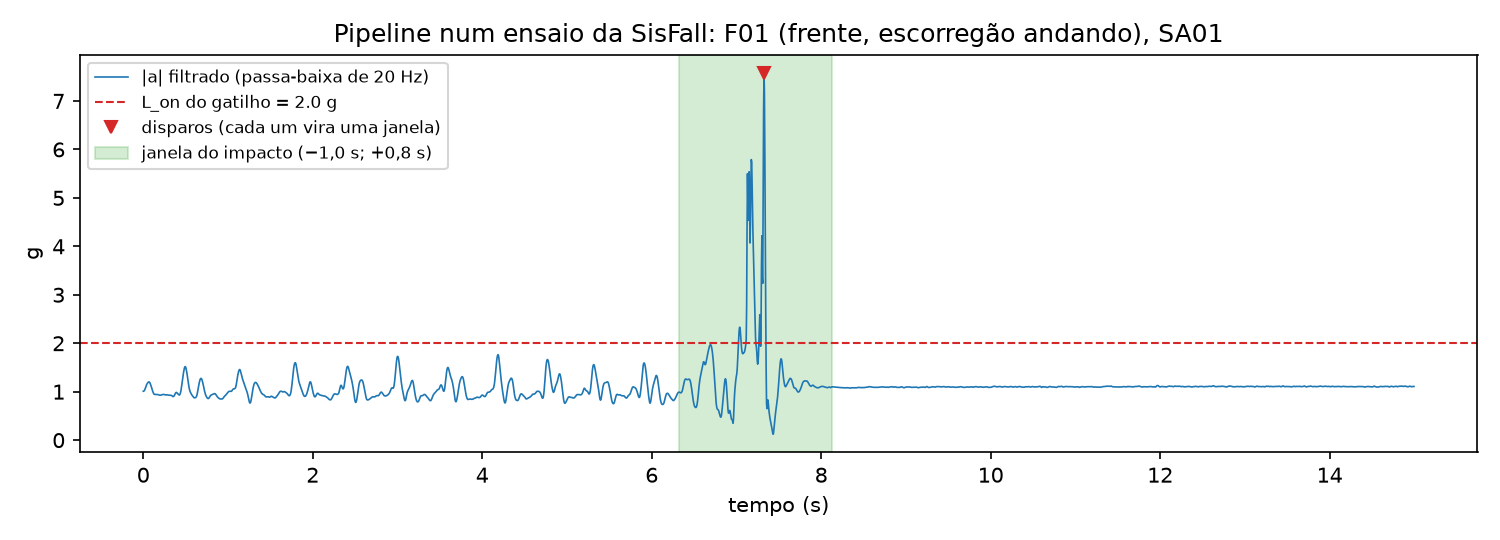
\includegraphics[width=\linewidth]{figuras/fig_pipeline.png}
\caption{O pipeline numa queda da SisFall: o sinal filtrado, o nível do gatilho e a janela
classificada em volta do impacto.}
\label{fig:pipeline}
\end{figure}

\begin{figure}[H]
\centering
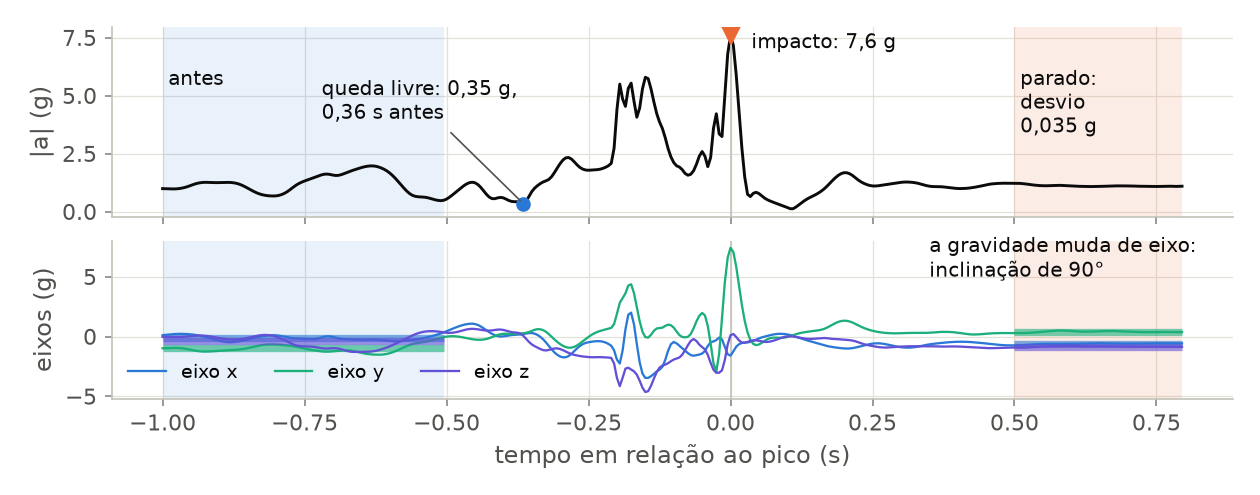
\includegraphics[width=\linewidth]{figuras/fig_janela.png}
\caption{A janela de uma queda e o que os atributos medem: a queda livre antes do impacto, o
impacto e o corpo parado em outra posição (a gravidade muda de eixo).}
\label{fig:janela}
\end{figure}

\subsection{A métrica: alarmes falsos por hora de atividade}\label{sec:metrica}

Um detector de queda erra de dois jeitos: deixa passar uma queda, ou chama o cuidador sem que
ninguém tenha caído. O primeiro erro se mede pela fração das quedas detectadas. O segundo, pelos
\textbf{alarmes falsos por hora de atividade}: quantas vezes o sistema chamaria o cuidador à toa
a cada hora em que o residente está se movimentando. As duas medidas andam juntas: baixar o
limiar pega mais quedas e dá mais alarmes, e subir faz o contrário.

\paragraph{Que horas são essas.} São as \adlHoras\,h de atividades da SisFall: os
\adlEnsaios{} ensaios sem queda, de \adlTipos{} tipos, feitos pelas \sisPessoas{} pessoas
(Tabela~\ref{tab:horas_atividade}). Cada tipo de ensaio tem uma duração prevista, de 100\,s
para andar e correr a 12\,s para os movimentos curtos, como sentar, deitar e agachar, e a soma
das durações de todos os ensaios é o denominador. São horas só de movimento, e de movimentos escolhidos para parecer queda: correr,
descer escada depressa, sentar de uma vez numa cadeira baixa, desabar na cadeira, tropeçar e
pular. Ficam de fora as horas paradas de um dia real, como dormir, comer e ver televisão, em
que o gatilho quase não dispara. Por isso, uma hora de atividade da SisFall gera mais alarmes
que uma hora qualquer do dia.

\begin{table}[H]
\centering
\caption{As horas de atividade da SisFall, o denominador da métrica.}
\label{tab:horas_atividade}
\small
% Gerado por modelo/experimentos/12_relatorio_q2.py a partir da SisFall (dados/publicos)
\begin{tabular}{@{}l l r r r r@{}}
\toprule
Atividades & Tipos & Ensaios & \makecell[r]{Cada ensaio\\(s)} & Horas & Parte \\
\midrule
Andar e correr & D01--D04 & 150 & 100 & 4,3 & 29\,\% \\
Subir e descer escada & D05--D06 & 308 & 25 & 2,1 & 15\,\% \\
Sentar e levantar da cadeira & D07--D11 & 940 & 12 & 3,1 & 22\,\% \\
Deitar e virar na cama & D12--D14 & 500 & 12 & 1,7 & 11\,\% \\
Agachar e curvar & D15--D16 & 380 & 12 & 1,3 & 9\,\% \\
Entrar e sair do carro & D17 & 189 & 25 & 1,3 & 9\,\% \\
Tropeçar e pular & D18--D19 & 240 & 12 & 0,8 & 5\,\% \\
\midrule
\textbf{Total} & 19 tipos & 2707 & & \textbf{14,5} & 100\,\% \\
\bottomrule
\end{tabular}

\end{table}

\paragraph{A conta.} Para o Random Forest da pulseira (Seção~\ref{sec:rf_pulseira}):
\begin{enumerate}
  \item Cada janela recebe a probabilidade dada por um modelo treinado sem a pessoa dela
        (validação cruzada por pessoa, em 5 dobras). Assim, o resultado vale para alguém que o
        modelo nunca viu.
  \item O gatilho abre \adlJanelas{} janelas nas atividades, \gatilhoDisparosH{} por hora, e
        \impactos{} janelas de impacto nas \quedasEnsaios{} quedas.
  \item O limiar é o que deixa 95\,\% das janelas de impacto acima dele: $P \ge \text{\rfLimiar}$.
  \item Com esse limiar, \rfAlarmesN{} das \adlJanelas{} janelas de atividade passam como
        queda. São os alarmes falsos:
        \[
          \frac{\text{\rfAlarmesN{} alarmes falsos}}{\text{\adlHoras\,h de atividade}}
          \approx \text{\rfAlarmes{} alarme falso por hora.}
        \]
  \item Nesse ponto, o modelo detecta \rfSensEnsaio\,\% das quedas. A conta é por queda, e não
        por janela: entram também as quedas que o gatilho perdeu, e por isso o número fica abaixo
        dos 95\,\%.
\end{enumerate}
A coluna ``Quedas com $\le$1 alarme/h'' da Tabela~\ref{tab:modelos_pulseira} faz a pergunta ao
contrário. Se o cuidador aceitar até um alarme falso por hora de atividade, ou seja,
\alarmesPermitidos{} nas \adlHoras\,h, o limiar pode descer até ficarem só
\alarmesPermitidos{} janelas de atividade acima dele. Quantas quedas passam então? Para o
Random Forest, \rfQuedas\,\%.

\paragraph{Por que essa métrica.}
\begin{itemize}
  \item \textbf{Mede o que custa na ILPI.} Cada alarme falso tira o cuidador de outro
        residente. Com alarmes demais, a equipe deixa de acreditar no sistema, e a queda de
        verdade também fica sem resposta. Contado por hora, o número vira alarmes por dia e por
        plantão: basta multiplicar pelas horas de atividade e pelo número de residentes.
  \item \textbf{Não engana como a acurácia.} Quase todas as janelas são de atividade, e um
        detector que nunca chama acerta quase todas elas. A especificidade por janela também
        engana. A do Random Forest é de \rfEspecJanela\,\%, o que parece perfeito, mas o número
        de alarmes depende de quantas janelas o gatilho abre: com o mesmo acerto por janela, um
        gatilho que abrisse dez vezes mais janelas daria dez vezes mais alarmes. Contados por
        hora, os alarmes já levam o gatilho em conta.
  \item \textbf{Compara métodos diferentes.} O AR, o DTW, a rede convolucional e os
        classificadores de atributos olham janelas de tamanhos diferentes, abertas em momentos
        diferentes. Dividir pelo tempo põe todos na mesma unidade.
  \item \textbf{Vem sempre com as quedas detectadas.} Zero alarme é fácil: basta nunca chamar.
        Por isso os métodos são comparados no mesmo ponto, o limiar que deixa 95\,\% das
        janelas de impacto acima dele, como num ponto da curva ROC.
  \item \textbf{Liga ao requisito.} O RNF08 pede no máximo um alarme falso por dia por
        residente (Tabela~\ref{tab:rnf}). Com \rfAlarmes{} alarme por hora de atividade, a conta
        fecha enquanto o residente tiver até \rnfHorasDia\,h por dia de movimento parecido com o
        da SisFall.
\end{itemize}

\paragraph{Limites.} A conta vale para os ensaios da SisFall: curtos, encenados em laboratório
e com o sensor na cintura. No pulso, o braço faz movimentos que a cintura não vê, como
gesticular e bater a mão na mesa, e eles também podem disparar o gatilho. A conversão para
alarmes por dia dá só a ordem de grandeza. A medida que vale é a do uso contínuo da pulseira,
prevista na verificação do RNF08.

\subsection{Comparação}

O Q1 comparou 22 métodos: os das aulas (modelos autorregressivos AR e ARX, correlação com
sinais de referência, DTW, atributos no tempo e em frequência, distâncias) e os usuais na
literatura (regras, regressão logística, árvore, SVM, Random Forest e redes convolucionais).
A avaliação é por pessoa: nenhuma pessoa aparece no treino e no teste ao mesmo tempo. A métrica
é a da Seção~\ref{sec:metrica}: alarmes falsos por hora de atividade, com cerca de 94\,\% das
quedas detectadas (Figura~\ref{fig:resumo}). O AR descreve bem a atividade normal, mas, usado como detector de
anomalia, dispara em qualquer movimento brusco; os métodos de atributos com um classificador
foram muito melhores.

\begin{figure}[H]
\centering
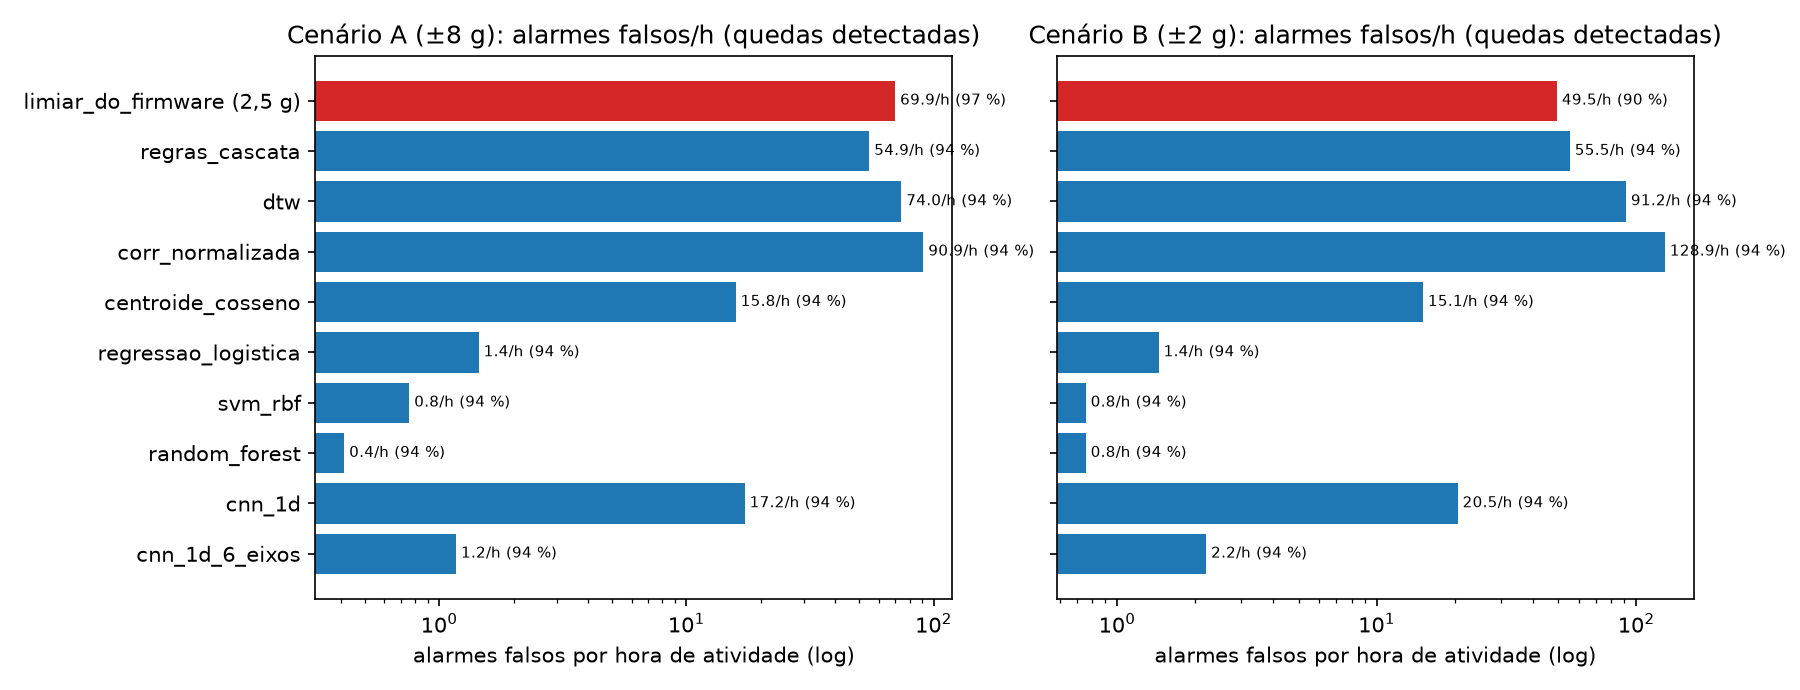
\includegraphics[width=\linewidth]{figuras/fig_resumo.png}
\caption{Alarmes falsos por hora de atividade de alguns dos métodos comparados no Q1, com a
fração de quedas detectadas entre parênteses. Cenário A: $\pm$8\,g, como a pulseira.}
\label{fig:resumo}
\end{figure}

\subsection{O modelo da pulseira}\label{sec:rf_pulseira}

Na configuração exata da pulseira (gatilho causal, os \nAtributos{} atributos no tempo,
$\pm$8\,g), três classificadores ficaram na disputa (Tabela~\ref{tab:modelos_pulseira}). As
diferenças entre eles cabem no erro da estimativa: os intervalos de 95\,\% das diferenças,
obtidos sorteando pessoas, passam pelo zero. O \textbf{Random Forest}~\cite{breiman} ficou: não precisa
padronizar os atributos, a probabilidade que vai no alerta é a fração de árvores que votaram
queda, e ele mostra quais atributos pesam (Figura~\ref{fig:importancia}). O SVM só entraria no
firmware se ganhasse com folga, porque exigiria outro classificador em C e outros testes.

\begin{table}[H]
\centering
\caption{Classificadores na configuração da pulseira (SisFall, validação por pessoa).}
\label{tab:modelos_pulseira}
\small
% Gerado por modelo/experimentos/12_relatorio_q2.py a partir de resultados/pulseira.json e svm_pulseira.json
\begin{tabular}{@{}lrrrr@{}}
\toprule
Classificador & \makecell[r]{Alarmes\\falsos/h} & \makecell[r]{Quedas com\\$\le$1 alarme/h} & \makecell[r]{Memória\\(kB)} & \makecell[r]{Operações\\por janela} \\
\midrule
Regressão logística & 0,62 & 94,9\,\% & 0,3 & 69 \\
Random Forest (60 árvores, prof. 10) & 0,55 & 95,1\,\% & 106,2 & 600 \\
SVM (RBF) & 0,69 & 96,2\,\% & 33,6 & 24\,012 \\
\bottomrule
\end{tabular}

\end{table}

\begin{figure}[H]
\centering
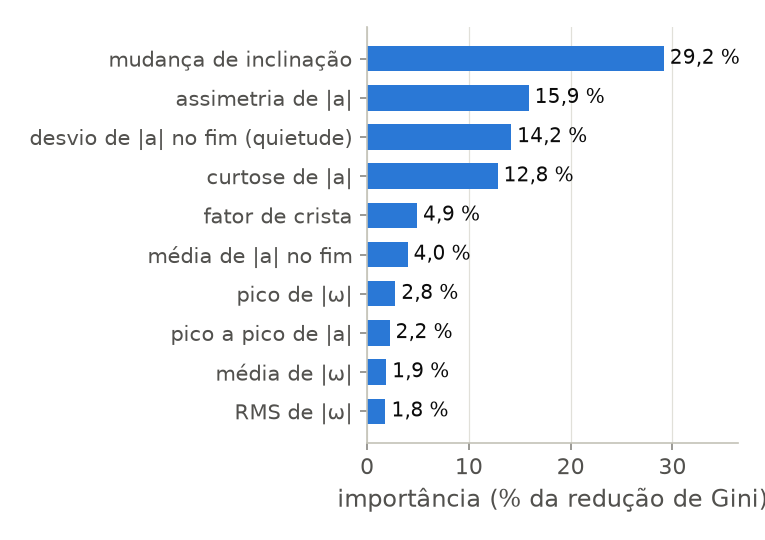
\includegraphics[width=0.9\linewidth]{figuras/fig_importancia.png}
\caption{Importância dos atributos no Random Forest da pulseira.}
\label{fig:importancia}
\end{figure}

O modelo tem 60 árvores de profundidade até 10 (\rfNos{} nós) e decide queda quando
$P \ge \text{\rfLimiar}$. No pipeline completo, sobre toda a SisFall, ele dá \rfAlarmes{} alarme falso
por hora de atividade e detecta \rfQuedas\,\% das quedas com no máximo um alarme falso por hora
(Figura~\ref{fig:funil}).

\begin{figure}[H]
\centering
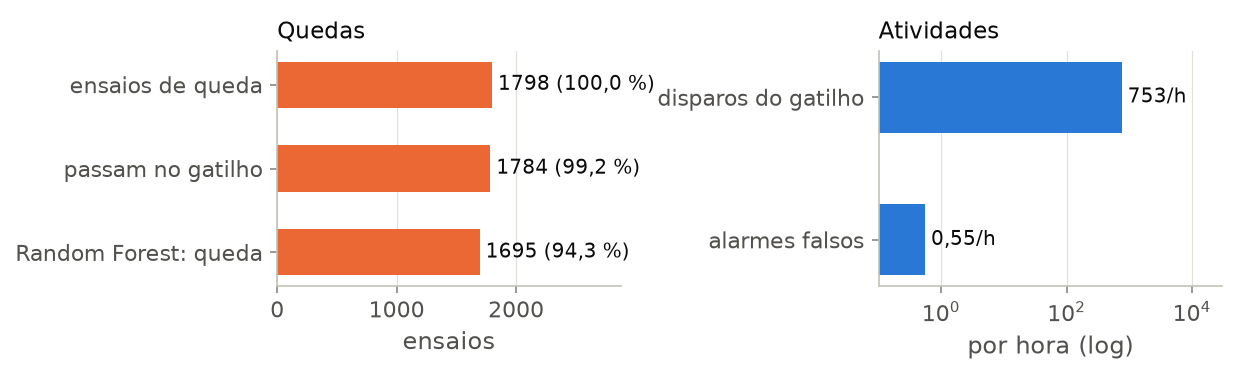
\includegraphics[width=\linewidth]{figuras/fig_funil_pulseira.png}
\caption{O pipeline da pulseira na SisFall: das quedas, quantas passam no gatilho e quantas o
Random Forest confirma; das atividades, quantos disparos e quantos alarmes falsos por hora.}
\label{fig:funil}
\end{figure}

\subsection{A versão embarcada}

O modelo vai para o firmware como código C gerado: um script Python exporta a floresta como
tabelas de nós (\rfBytes{} bytes de flash), os coeficientes do filtro, o gatilho e o limiar, e
gera junto os vetores de teste. O pipeline em C roda amostra a amostra na task
\code{sampling}, com o filtro do ESP-DSP e um buffer circular por eixo; a janela só é
classificada quando o gatilho dispara. O custo em ciclos de cada classificação é medido e vai
para o log.

A garantia de que o C faz o mesmo que o Python é o teste de paridade: em 26 janelas de 8
trechos da SisFall, o C acha os mesmos picos, calcula os atributos dentro da tolerância e dá
a mesma probabilidade, até $10^{-6}$ (885 verificações, Tabela~\ref{tab:testes}). Na placa, o
modo de coleta permite a mesma comparação com o sinal real do sensor: ele manda o sinal bruto
e cada janela classificada pela serial, para o Python refazer as contas.

\subsection{Nos nossos ensaios e limitações}

Nos 18 ensaios do primeiro semestre, o Random Forest treinado só na SisFall não deu nenhum
alarme ao andar ou correr e pegou as quedas de frente e de costas, mas perdeu as três quedas de
joelhos (Figura~\ref{fig:proprios}). São poucos ensaios, de uma pessoa só, mas o tipo de
queda que falhou fica marcado para a coleta.

\begin{figure}[H]
\centering
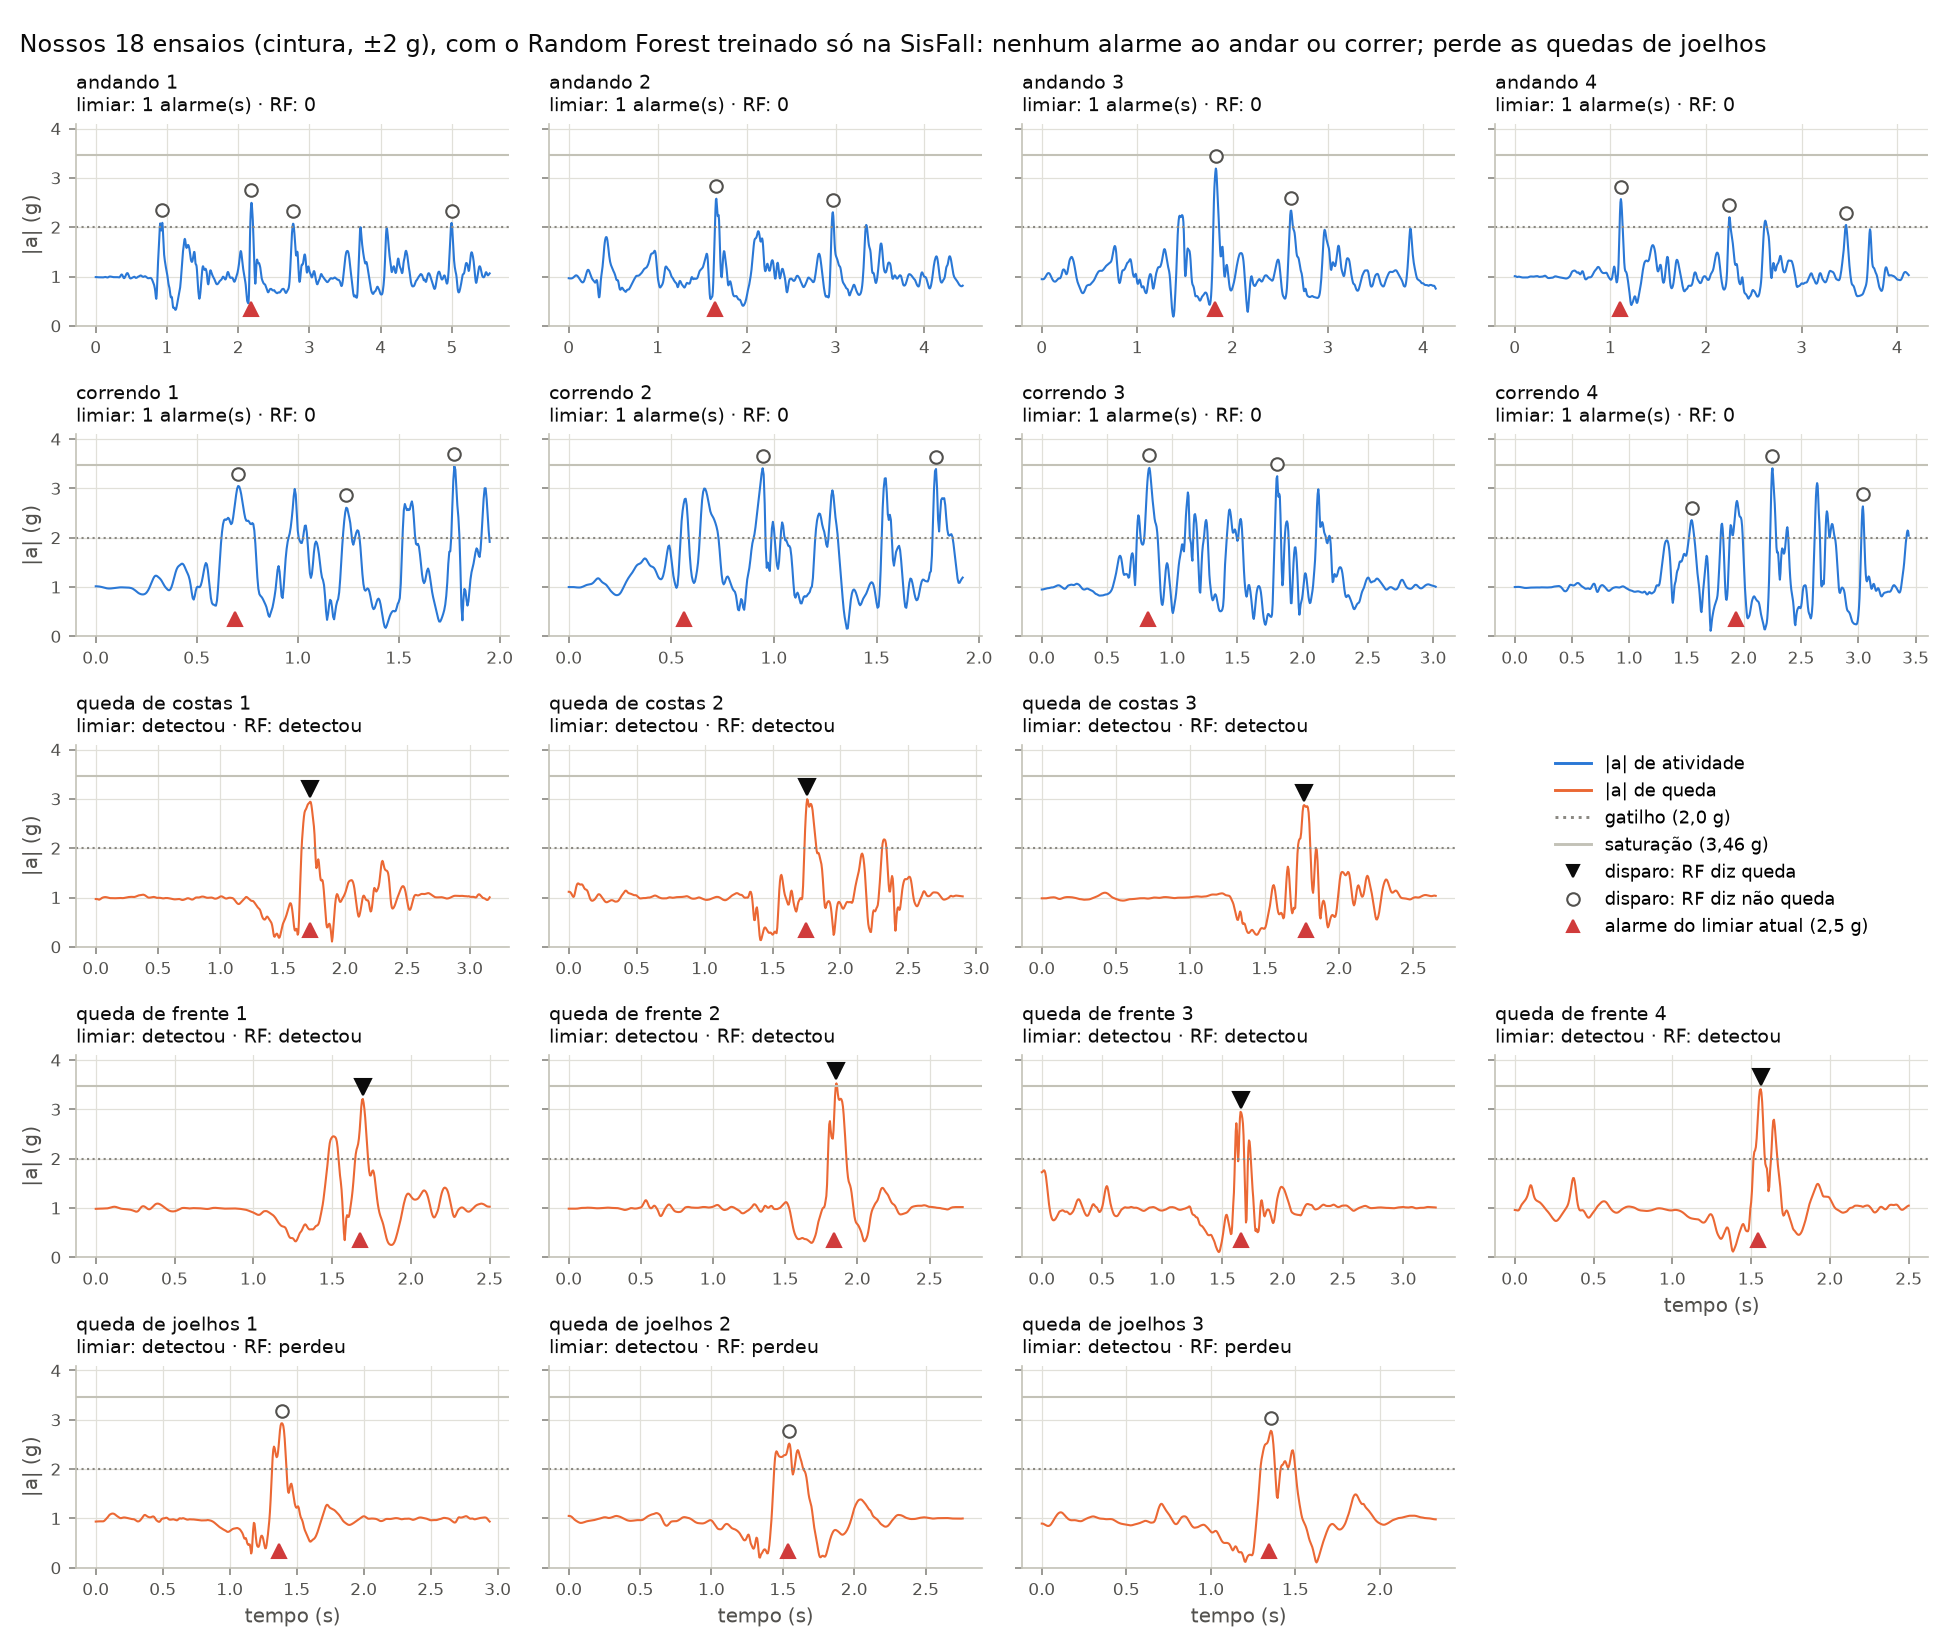
\includegraphics[width=\linewidth]{figuras/fig_proprios_ensaios.png}
\caption{Os 18 ensaios do primeiro semestre com o Random Forest treinado na SisFall.}
\label{fig:proprios}
\end{figure}

O modelo é \textbf{provisório}. Os dados de treino têm o sensor na cintura, e a pulseira vai no
pulso, onde o braço se move muito mais e o impacto chega diferente. O próximo passo é a coleta
no pulso, com várias pessoas e com o firmware atual ($\pm$8\,g), seguindo o protocolo de coleta
do projeto: os ensaios gravados pelo modo de coleta entram direto no treino, e o mesmo script
gera o novo modelo e os novos vetores de teste. Com esses dados, também vale reavaliar os
atributos de frequência, que na cintura melhoraram o resultado mas exigiriam uma FFT no
firmware.

	%======================================================================
\section{Central}\label{sec:central}
%======================================================================
A central recebe o que os hubs publicam, guarda o histórico, mostra os quartos e avisa o
cuidador. Ela não decide nada: as regras e os alertas chegam prontos das placas. Tudo roda em
contêineres Docker, descritos num único arquivo do Docker Compose, num PC ou num Raspberry Pi 4
(Tabela~\ref{tab:central}).

\begin{table}[H]
\centering
\caption{Serviços da central.}
\label{tab:central}
\small
\begin{tabular}{@{}l>{\raggedright\arraybackslash}p{11.8cm}@{}}
\toprule
Serviço & Função \\
\midrule
Mosquitto & broker MQTT com usuário e senha por cliente e ACL por tópico (Seção~\ref{sec:mqtt}) \\
Telegraf & assina \code{idoso/\#} e grava cada mensagem no InfluxDB, com o site, o quarto e o identificador como \textit{tags}; sem código próprio \\
InfluxDB & banco de séries temporais, com retenção de 30 dias \\
Grafana & painel ``Quartos'', com seletor de quarto; o painel é versionado em JSON no repositório \\
Notificador & programa em Python que assina \code{idoso/+/+/alerta} e envia cada alerta ao Telegram do cuidador \\
\midrule
Simulador & programa em Python que faz o papel de um hub, para testar a central sem hardware \\
\code{demo\_pulseira.py} & demonstração da pulseira com uma placa só, pela USB (Seção~\ref{sec:demo}) \\
\bottomrule
\end{tabular}
\end{table}

\subsection{Painel}

O painel ``Quartos'' mostra, para o quarto escolhido: o estado do hub (online ou offline, pelo
\textit{Last Will}), a presença, a temperatura atual e o histórico, as portas, o estado da
pulseira, a linha do tempo de portas e presença, a tabela de alertas (com a probabilidade de
queda dada pela pulseira), a bateria e o nível de atividade da pulseira
(Figura~\ref{fig:grafana}). As consultas foram testadas com o simulador; a aparência com dados
reais ainda vai ser conferida.

\begin{figure}[H]
\centering
\fotoouespaco{grafana_quartos}{0.95\linewidth}{captura do painel ``Quartos'' do Grafana com dados do hub (ou do simulador)}
\caption{Painel ``Quartos'' no Grafana.}
\label{fig:grafana}
\end{figure}

\subsection{Notificador}

O notificador transforma cada alerta numa mensagem legível (tipo, quarto e horário) e a manda
pelo Telegram. Ele foi feito para não perder alertas:
\begin{itemize}
  \item a sessão MQTT é persistente: os alertas publicados enquanto ele estava fora do ar
        chegam quando ele volta;
  \item se o Telegram não aceitar a mensagem (sem internet, por exemplo), ele espera e tenta de
        novo, com espera crescente até 60\,s; só uma mensagem recusada pelo próprio Telegram
        é descartada;
  \item \code{id} e \code{estado} repetidos (QoS 1) são descartados;
  \item um alerta com dados inesperados vira uma mensagem simples, em vez de derrubar o
        programa.
\end{itemize}

\begin{figure}[H]
\centering
\fotoouespaco{telegram_alerta}{0.42\linewidth}{captura do celular com um alerta de queda no Telegram}
\caption{Alerta de queda chegando ao cuidador pelo Telegram.}
\label{fig:telegram}
\end{figure}

\subsection{Demonstração com uma placa}\label{sec:demo}

Para mostrar o modelo de queda funcionando sem montar o sistema todo, a pulseira tem um perfil
de demonstração: sem hub, com o modo de coleta ligado e a serial a 921\,600\,baud. No
computador, o \code{demo\_pulseira.py} lê a serial e mostra, ao vivo, o $\amag$ filtrado, cada
disparo do gatilho com a probabilidade dada pelo modelo e uma faixa ``QUEDA DETECTADA'' quando
a pulseira decide queda. Opcionalmente, ele faz o papel do hub e publica o alerta no broker,
no mesmo formato, e o alerta aparece no Grafana e no Telegram. Se o link USB cair, a leitura
reabre a porta sozinha.

\begin{figure}[H]
\centering
\fotoouespaco{demo_pulseira}{0.85\linewidth}{janela do demo\_pulseira.py durante uma queda simulada}
\caption{A janela da demonstração com uma placa.}
\label{fig:demo}
\end{figure}

	%======================================================================
\section{Verificação e plano de testes}\label{sec:verificacao}
%======================================================================
\subsection{Níveis de verificação}

A verificação do sistema é feita em três níveis (Tabela~\ref{tab:niveis}), dos testes
automáticos no computador até os testes na placa, com os sensores.

\begin{table}[H]
\centering
\caption{Níveis de verificação.}
\label{tab:niveis}
\small
\begin{tabular}{@{}l>{\raggedright\arraybackslash}p{11.0cm}@{}}
\toprule
Nível & Significa \\
\midrule
testes no PC & testes automáticos rodando no computador (lógica pura, sem placa) \\
ponta a ponta sem placa & central real em Docker, com o simulador no lugar do hub \\
bancada & rodando na placa, com os sensores \\
\bottomrule
\end{tabular}
\end{table}

\subsection{Verificações realizadas}

\begin{table}[H]
\centering
\caption{Como cada parte foi verificada.}
\label{tab:verificado}
\small
\begin{tabular}{@{}>{\raggedright\arraybackslash}p{4.0cm}>{\raggedright\arraybackslash}p{9.8cm}@{}}
\toprule
Parte & Como \\
\midrule
Firmware do hub & testes no computador das regras de alerta (82 verificações), da configuração por MQTT (60) e do envio por mudança (23) \\
Firmware da pulseira & testes no computador do pipeline de queda (885 verificações, com a paridade C $\times$ Python), do processamento de sinal (25) e dos gestos do botão (42) \\
Mapa de pinos, chaves e MAC & pino repetido ou proibido e MAC mal escrito fazem o build falhar \\
Modelo de queda & validação por pessoa na SisFall; paridade C $\times$ Python \\
Central & os 5 serviços sobem; o broker recusa conexão anônima e senha errada; o simulador publicou estados e alertas, o InfluxDB gravou, as consultas do painel rodaram e o notificador formatou cada episódio \\
Notificador e demonstração & 22 e 19 testes automáticos \\
PCB v1 & \ercViolacoes{} violações de ERC e \drcErros{} erros de DRC; encaixe e ordem dos pinos no teste no papel 1:1 \\
Pulseira na placa & perfil de demonstração: 200\,Hz contínuos por 16\,min e $\pm$8\,g confirmado (abaixo) \\
\bottomrule
\end{tabular}
\end{table}

\paragraph{Pulseira na placa.} Em 13/11/2026, a pulseira com o perfil de demonstração,
ligado ao computador por USB, mandou as amostras brutas a 200\,Hz por 16 minutos sem parar.
Parado, $\amag$ ficou em $\approx$4077 contagens, ou seja, $\approx$1\,g na escala de
4096 contagens por g: a faixa de $\pm$8\,g está configurada. No mesmo ensaio, o programa de
demonstração parou de atualizar quando o link USB piscou, e a leitura da serial foi corrigida
para reabrir a porta sozinha.

\subsection{Plano de testes em bancada}

A Tabela~\ref{tab:plano} lista os testes na placa, com os sensores, na ordem em que fazem
sentido, com o critério de aprovação. As metas vêm dos requisitos (Seção~\ref{sec:requisitos}).

\begin{table}[H]
\centering
\caption{Plano de testes em bancada.}
\label{tab:plano}
\small
\begin{tabular}{@{}>{\raggedright\arraybackslash}p{2.7cm}>{\raggedright\arraybackslash}p{6.0cm}>{\raggedright\arraybackslash}p{5.1cm}@{}}
\toprule
Teste & Procedimento & Critério \\
\midrule
Amostragem & modo de coleta; intervalos entre amostras & 200\,Hz, \textit{jitter} $\le \pm$5\,ms (RNF01) \\
Faixa do MPU & placa parada; uma batida forte & $\sim$4096 contagens no eixo vertical; batida acima de 3,46\,g sem teto plano \\
Pipeline na placa & balançar; soltar a placa numa almofada; comparar o CSV bruto com o Python & disparos com P baixa; queda detectada; mesmos picos e mesma P do computador \\
Portas & abrir e fechar depressa, várias vezes & nenhuma transição perdida ou inventada \\
PIR & movimento depois dos 60\,s de aquecimento & detecção e volta a ``livre'' \\
Temperatura & 3 ou 4 pontos (perto de 10, 20 e 30\,°C) contra um termômetro; depois, termopar; 30\,min com o quarto parado & $\pm$1\,°C (RNF10); parado, o ruído fica abaixo de 0,2\,°C e sai uma mensagem a cada 5\,min \\
Peças ausentes & sem SSID, senha errada, broker parado, LM35 solto, MPU solto, CAN sem transceptor & um aviso por caso, e o resto funcionando \\
CAN entre as placas & pulseira com CAN de bancada, transceptores e terminação; tirar um fio do barramento & quadros \code{0x0FD}/\code{0x0FE} no log do hub; um aviso ao cair e um ao voltar \\
Botão & aperto simples; dois toques sem alerta; dois toques na janela de uma queda; segurar 3\,s; segurar durante um alerta; ficar com o botão apertado por 30\,s & só os dois toques na janela cancelam e só o segurar fora de alerta pede ajuda; o resto não faz nada; segurar sem soltar dá um pedido só \\
ESP-NOW & boot da pulseira; queda simulada (dois toques, opção de teste); ``estou bem''; pedido de ajuda & canal descoberto; heartbeat no Grafana; alertas \code{queda} e \code{ajuda}, \code{ativo} e \code{cancelado} \\
Queda atrasada & hub desligado, queda, hub religado em $\sim$20\,s & o alerta chega uma vez só \\
Queda após reinício & queda, pulseira reiniciada, nova queda & dois alertas, com \code{id} diferentes \\
Remetente estranho & outro ESP32 mandando ESP-NOW ao hub & um aviso e nenhum alerta \\
Latências & hora na pulseira, no hub, no broker e no celular & pico $\to$ MQTT $\le$ 500\,ms; porta $\to$ MQTT $\le$ 200\,ms; alerta $\to$ Telegram $\le$ 5\,s \\
\textit{Last Will} & desligar o hub & \code{status} \code{offline} em até $\sim$45\,s \\
Notificador & derrubar a internet 1\,min com um alerta no meio; reiniciar o contêiner & os dois alertas chegam \\
Disponibilidade & 24\,h contínuas, derrubando a rede & reconexão sozinha, nenhum evento QoS 1 perdido \\
Autonomia & medidor USB entre o \textit{power bank} e a pulseira & consumo medido (RNF14) \\
\bottomrule
\end{tabular}
\end{table}

	%======================================================================
\section{Conclusões}\label{sec:conclusoes}
%======================================================================
\subsection{Situação}

O sistema está projetado de ponta a ponta e, na maior parte, implementado
(Tabela~\ref{tab:objetivos}). Os sensores foram escolhidos e caracterizados; o condicionamento
do LM35 foi projetado, simulado e validado, e na placa nova passou a funcionar com uma
alimentação só e um filtro na entrada do ADC; a PCB única foi desenhada, verificada e
fabricada; o firmware das duas placas está completo e compila sem avisos; a detecção de queda
passou de um limiar a um modelo embarcado; e a central funciona com um simulador no lugar do
hub. O que falta é sobretudo bancada: montar a placa e verificar, com o hardware real, o que
hoje está verificado só no computador.

\begin{table}[H]
\centering
\caption{Objetivos específicos e situação.}
\label{tab:objetivos}
\small
\begin{tabular}{@{}>{\raggedright\arraybackslash}p{6.4cm}>{\raggedright\arraybackslash}p{7.4cm}@{}}
\toprule
Objetivo & Situação \\
\midrule
Selecionar e caracterizar os sensores & feito (primeiro semestre); a faixa do MPU passou a $\pm$8\,g, confirmada na placa \\
Condicionar o LM35 & feito e validado em protoboard; falta conferir na PCB v1 \\
PCB única & desenhada, verificada (ERC e DRC) e fabricada; falta montar e testar \\
Rede CAN & firmware pronto e validado com o professor numa versão anterior; falta o teste entre as placas v1 \\
Interface sem fio e contrato MQTT & firmware pronto, contrato documentado; falta o teste ESP-NOW em bancada \\
Detecção de queda embarcada & modelo no firmware, com paridade C $\times$ Python; provisório até os dados do pulso \\
Regras e alertas no hub & prontas e testadas no computador \\
Histórico, painel e notificação & funcionando com o simulador; falta o bot do Telegram com o celular do cuidador \\
\bottomrule
\end{tabular}
\end{table}

\subsection{Limitações}

\begin{itemize}
  \item O modelo de queda foi treinado com o sensor na cintura, e o vestível vai no pulso.
  \item Nada do sistema completo foi verificado em bancada ainda: as metas de latência,
        disponibilidade e autonomia estão definidas, mas não medidas.
  \item A exatidão da temperatura na placa nova ainda não foi conferida contra um termopar.
  \item O vestível usa a mesma placa do hub: é grande e depende de um \textit{power bank}, sem
        medição de bateria.
  \item A cobertura do ESP-NOW fica limitada ao raio do hub; o corredor e as áreas comuns
        estão fora do escopo desta fase.
\end{itemize}

\subsection{Próximos passos}

\begin{enumerate}
  \item Montar as placas v1 e fazer os testes da Seção~\ref{sec:verificacao}, começando pelo
        ESP-NOW entre o vestível e o hub, para a apresentação do Q3 (24/11).
  \item Coletar quedas e atividades com o vestível no pulso, com várias pessoas, e retreinar
        o modelo; reavaliar ali os atributos de frequência e o SVM.
  \item Medir o consumo e implementar o \textit{light sleep} no vestível.
  \item Uma placa própria para o vestível, com bateria LiPo, carregador e medição da bateria.
  \item Na central: um servidor NTP local, para a ILPI funcionar sem internet; um painel para
        a telemetria do vestível; e um banco relacional (PostgreSQL) com residentes,
        dispositivos, cuidadores e o ciclo de vida dos alertas.
\end{enumerate}


	\begin{thebibliography}{99}
\bibitem{q1} GARCIA, D.; MARGARIDO, H. G.; SANTIAGO, H. \emph{Projeto 3 --- Entrega Q1:
  modelos autorregressivos e de classificação para a detecção de quedas na pulseira}.
  Relatório da disciplina 0323221 - Projeto Integrativo 3. Escola Politécnica da USP, 2026.
\bibitem{sisfall} SUCERQUIA, A.; LÓPEZ, J. D.; VARGAS-BONILLA, J. F. SisFall: a fall
  and movement dataset. \emph{Sensors}, v.~17, n.~1, p.~198, 2017.
\bibitem{mpu6050} INVENSENSE. \emph{MPU-6000 and MPU-6050 product specification}.
  Revisão 3.4, 2013.
\bibitem{lm35} TEXAS INSTRUMENTS. \emph{LM35 precision centigrade temperature sensors}.
  Folha de dados SNIS159.
\bibitem{lm358} TEXAS INSTRUMENTS. \emph{LMx58, LM2904 dual operational amplifiers}.
  Folha de dados SLOS068.
\bibitem{hcsr501} \emph{HC-SR501 PIR motion detector}. Folha de dados do módulo.
\bibitem{sn65hvd230} TEXAS INSTRUMENTS. \emph{SN65HVD23x 3.3-V CAN bus transceivers}.
  Folha de dados SLOS346.
\bibitem{esp32s3} ESPRESSIF SYSTEMS. \emph{ESP32-S3 series datasheet} e \emph{ESP32-S3
  technical reference manual}. 2025.
\bibitem{espidf} ESPRESSIF SYSTEMS. \emph{ESP-IDF programming guide}, versão 6.0.1, para o
  ESP32-S3. Disponível em: \url{https://docs.espressif.com/projects/esp-idf}.
\bibitem{espnow} ESPRESSIF SYSTEMS. ESP-NOW. In: \emph{ESP-IDF programming guide}, versão
  6.0.1.
\bibitem{mqtt} OASIS. \emph{MQTT version 3.1.1}. OASIS Standard, 2014.
\bibitem{iso11898} INTERNATIONAL ORGANIZATION FOR STANDARDIZATION. \emph{ISO 11898-1: road
  vehicles --- controller area network (CAN)}. Genebra: ISO, 2015.
\bibitem{breiman} BREIMAN, L. Random forests. \emph{Machine Learning}, v.~45, n.~1,
  p.~5--32, 2001.
\bibitem{slides} Slides da disciplina: ``ESP32 - GPIO'', ``ESP32 - ADC'', ``ESP32 - RTOS'',
  ``ESP32 - CAN'', ``ESP32 - Amostragem'' e ``CEM: projeto de PCB''. Escola Politécnica da
  USP, 2026.
\end{thebibliography}


	\appendix
	%======================================================================
\section{Esquemático completo}\label{ap:esquema}
%======================================================================
As folhas do esquemático da PCB v1, na ordem do arquivo do KiCad, recortadas no circuito
(sem a moldura e o carimbo). A folha principal está na Figura~\ref{fig:esquema_raiz}; o arquivo
completo, em PDF, fica em \code{hardware/placas/v1/esquema.pdf}.

\begin{figure}[H]
\centering
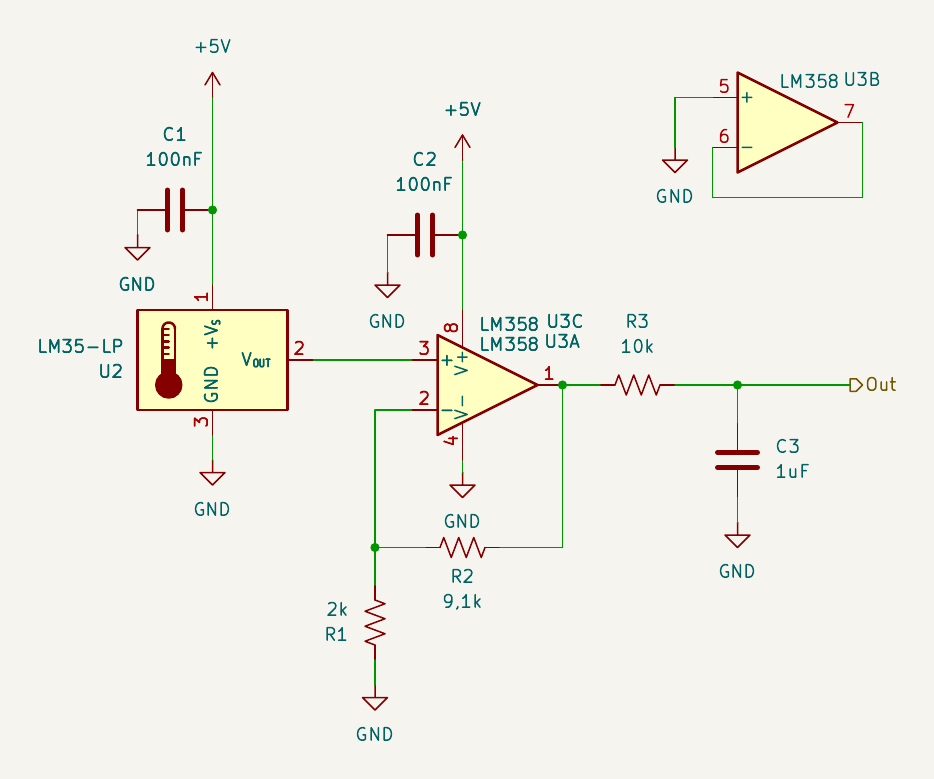
\includegraphics[scale=1.3]{figuras/esquema_p2.png}
\caption{Folha do LM35: sensor, LM358 (as duas metades) e filtro RC.}
\end{figure}

\begin{figure}[H]
\centering
\begin{subfigure}[b]{0.56\linewidth}
  \centering
  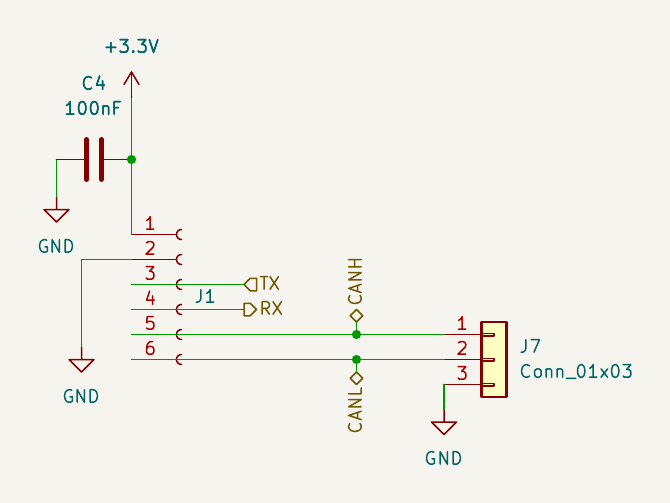
\includegraphics[scale=1.3]{figuras/esquema_p3.png}
  \caption{CAN: módulo transceptor (J1) e conector do barramento (J7).}
\end{subfigure}\hfill
\begin{subfigure}[b]{0.40\linewidth}
  \centering
  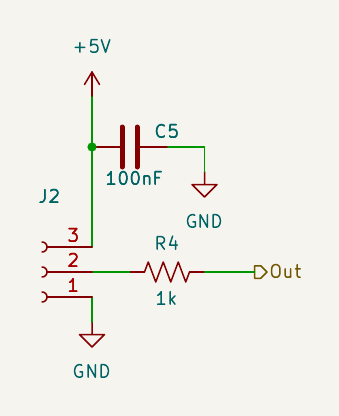
\includegraphics[scale=1.3]{figuras/esquema_p4.png}
  \caption{PIR HC-SR501 (J2), com R4 em série.}
\end{subfigure}
\caption{Folhas do CAN e do PIR.}
\end{figure}

\begin{figure}[H]
\centering
\begin{subfigure}[b]{0.24\linewidth}
  \centering
  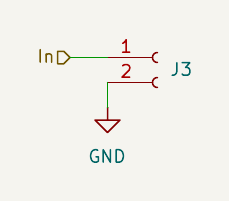
\includegraphics[scale=1.3]{figuras/esquema_p5.png}
  \caption{Porta 1 (J3).}
\end{subfigure}\hfill
\begin{subfigure}[b]{0.24\linewidth}
  \centering
  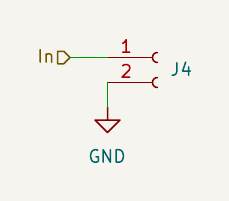
\includegraphics[scale=1.3]{figuras/esquema_p6.png}
  \caption{Porta 2 (J4).}
\end{subfigure}\hfill
\begin{subfigure}[b]{0.40\linewidth}
  \centering
  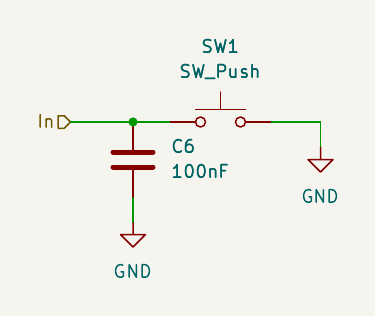
\includegraphics[scale=1.3]{figuras/esquema_p7.png}
  \caption{Botão da pulseira (SW1).}
\end{subfigure}

\vspace{4mm}
\begin{subfigure}[b]{0.40\linewidth}
  \centering
  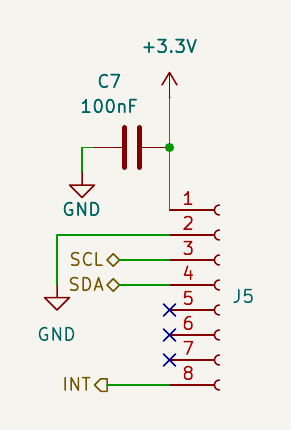
\includegraphics[scale=1.3]{figuras/esquema_p8.png}
  \caption{MPU-6050 (J5).}
\end{subfigure}\hfill
\begin{subfigure}[b]{0.40\linewidth}
  \centering
  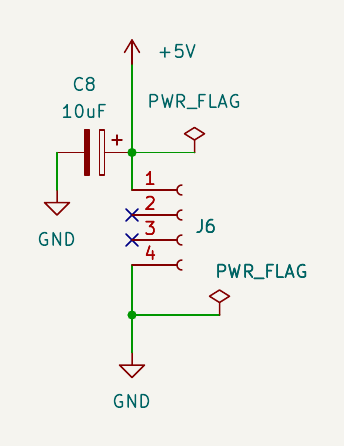
\includegraphics[scale=1.3]{figuras/esquema_p9.png}
  \caption{Entrada USB-C (J6).}
\end{subfigure}
\caption{Folhas das portas, do botão, do MPU-6050 e da alimentação.}
\end{figure}

%======================================================================
\section{Mapa de pinos completo}\label{ap:pinos}
%======================================================================
\begin{table}[H]
\centering
\caption{Mapa de pinos da PCB v1 (\code{firmware/common/pcb/include/pcb\_pins.h}).}
\label{tab:pinos_completo}
\small
\begin{tabular}{@{}l>{\raggedright\arraybackslash}p{5.0cm}l>{\raggedright\arraybackslash}p{5.2cm}@{}}
\toprule
GPIO & Função & Placa & Observação \\
\midrule
1 & I²C SDA (MPU-6050) & pulseira & par do ULP; ADC1, canal 0, usado como digital \\
2 & I²C SCL & pulseira & par do ULP; ADC1, canal 1 \\
4 & LM35 (saída do LM358) & hub & ADC1, canal 3 \\
5 & reservado: bateria de uma pulseira própria & --- & ADC1, canal 4; sem divisor nesta PCB \\
6, 7 & reserva analógica & --- & ADC1, canais 5 e 6 \\
8 & PIR HC-SR501 & hub & ADC1, canal 7, usado como digital \\
9, 10 & portas 3 e 4 (opcionais) & hub & ADC1, canais 8 e 9 \\
11, 12 & portas 1 (quarto) e 2 (banheiro) & hub & ADC2, mas digitais \\
13, 14 & CAN TX e RX & os dois & na pulseira, só em bancada \\
15, 16 & não ligar: cristal de 32\,kHz & --- & reserva \\
17 & interrupção do MPU-6050 & pulseira & RTC GPIO \\
18 & botão da pulseira & pulseira & RTC GPIO; \textit{pull-up} interno e filtro de \textit{glitch} \\
21 & livre (era o buzzer) & --- & \\
38 ou 48 & LED WS2812 & os dois & o da DevKit (v1.1 ou v1.0), escolhido no \code{menuconfig} \\
39--42 & expansão (por exemplo, portas 5 a 8) & --- & só enquanto o JTAG por pinos não for usado \\
\bottomrule
\end{tabular}
\end{table}

Para acrescentar uma porta, basta uma linha na tabela \code{BOARD\_DOORS} do hub: o firmware
cria a entrada, o tópico \code{porta/<id>} e o identificador CAN. São até 8 portas, uma por
identificador (\code{0x0F3} a \code{0x0FA}); o build falha se passar disso.

%======================================================================
\section{Lista de materiais e custo}\label{ap:bom}
%======================================================================
\begin{table}[H]
\centering
\caption{Lista de materiais da PCB v1 (gerada do KiCad).}
\label{tab:bom}
\footnotesize
% Gerado por modelo/experimentos/12_relatorio_q2.py a partir de hardware/placas/v1/lista-de-materiais.csv
\begin{tabular}{@{}l >{\raggedright\arraybackslash}p{2.3cm} >{\raggedright\arraybackslash}p{4.4cm} >{\raggedright\arraybackslash}p{4.4cm} r@{}}
\toprule
Referência & Valor & Função & Footprint & Qtd \\
\midrule
C1,C2,C4-C7 & 100\,nF & desacoplamento (LM35, LM358, CAN, PIR, botão, MPU) & \texttt{\scriptsize C\_\allowbreak{}Disc\_\allowbreak{}D3.0mm\_\allowbreak{}W1.6mm\_\allowbreak{}P2.50mm} & 6 \\
C3 & 1\,µF & filtro RC na entrada do ADC (com R3) & \texttt{\scriptsize C\_\allowbreak{}Rect\_\allowbreak{}L4.0mm\_\allowbreak{}W2.5mm\_\allowbreak{}P2.50mm} & 1 \\
C8 & 10\,µF & reservatório na entrada de 5 V & \texttt{\scriptsize CP\_\allowbreak{}Radial\_\allowbreak{}D5.0mm\_\allowbreak{}P2.00mm} & 1 \\
D1 & 1N5819 & impede juntar duas fontes no 5 V da DevKit & \texttt{\scriptsize D\_\allowbreak{}DO-41\_\allowbreak{}SOD81\_\allowbreak{}P10.16mm\_\allowbreak{}Horizontal} & 1 \\
J1 & Conn\_\allowbreak{}01x06\_\allowbreak{}Socket & módulo transceptor CAN SN65HVD230 & \texttt{\scriptsize WCMCU-230} & 1 \\
J2 & Conn\_\allowbreak{}01x03\_\allowbreak{}Socket & módulo PIR HC-SR501 & \texttt{\scriptsize HCSR501} & 1 \\
J3,J4 & Conn\_\allowbreak{}01x02\_\allowbreak{}Socket & portas 1 e 2 (reed MC-38) & \texttt{\scriptsize PinSocket\_\allowbreak{}1x02\_\allowbreak{}P2.54mm\_\allowbreak{}Vertical} & 2 \\
J5 & Conn\_\allowbreak{}01x08\_\allowbreak{}Socket & módulo MPU-6050 (GY-521) & \texttt{\scriptsize MPU6050} & 1 \\
J6 & Conn\_\allowbreak{}01x04\_\allowbreak{}Socket & módulo USB-C (entrada de 5 V) & \texttt{\scriptsize Modulo USB-C} & 1 \\
J7 & Conn\_\allowbreak{}01x03 & barramento CAN (CANH, CANL, GND) & \texttt{\scriptsize PinHeader\_\allowbreak{}1x03\_\allowbreak{}P2.54mm\_\allowbreak{}Vertical} & 1 \\
R1 & 2k & ganho do LM358 (para o GND) & \texttt{\scriptsize R\_\allowbreak{}Axial\_\allowbreak{}DIN0207\_\allowbreak{}L6.3mm\_\allowbreak{}D2.5mm\_\allowbreak{}P10.16mm\_\allowbreak{}Horizontal} & 1 \\
R2 & 9,1k & ganho do LM358 (realimentação) & \texttt{\scriptsize R\_\allowbreak{}Axial\_\allowbreak{}DIN0207\_\allowbreak{}L6.3mm\_\allowbreak{}D2.5mm\_\allowbreak{}P10.16mm\_\allowbreak{}Horizontal} & 1 \\
R3 & 10k & filtro RC (com C3) & \texttt{\scriptsize R\_\allowbreak{}Axial\_\allowbreak{}DIN0207\_\allowbreak{}L6.3mm\_\allowbreak{}D2.5mm\_\allowbreak{}P10.16mm\_\allowbreak{}Horizontal} & 1 \\
R4 & 1k & série na saída do PIR & \texttt{\scriptsize R\_\allowbreak{}Axial\_\allowbreak{}DIN0207\_\allowbreak{}L6.3mm\_\allowbreak{}D2.5mm\_\allowbreak{}P10.16mm\_\allowbreak{}Horizontal} & 1 \\
SW1 & SW\_\allowbreak{}Push & botão ``estou bem'' & \texttt{\scriptsize SW\_\allowbreak{}PUSH-12mm} & 1 \\
TP1 & 5V & ponto de teste & \texttt{\scriptsize TestPoint\_\allowbreak{}Pad\_\allowbreak{}D1.5mm} & 1 \\
TP2 & 3V3 & ponto de teste & \texttt{\scriptsize TestPoint\_\allowbreak{}Pad\_\allowbreak{}D1.5mm} & 1 \\
TP3 & GND & ponto de teste & \texttt{\scriptsize TestPoint\_\allowbreak{}Pad\_\allowbreak{}D1.5mm} & 1 \\
TP4 & LM35 & ponto de teste (saída do LM358) & \texttt{\scriptsize TestPoint\_\allowbreak{}Pad\_\allowbreak{}D1.5mm} & 1 \\
TP5 & CANH & ponto de teste & \texttt{\scriptsize TestPoint\_\allowbreak{}Pad\_\allowbreak{}D1.5mm} & 1 \\
TP6 & CANL & ponto de teste & \texttt{\scriptsize TestPoint\_\allowbreak{}Pad\_\allowbreak{}D1.5mm} & 1 \\
U1 & ESP32-S3-DevKitC & ESP32-S3-DevKitC-1 encaixada & \texttt{\scriptsize ESP32-S3-DevKitC} & 1 \\
U2 & LM35-LP & sensor de temperatura LM35DZ & \texttt{\scriptsize TO-92\_\allowbreak{}Inline\_\allowbreak{}Wide} & 1 \\
U3 & LM358 & amp-op LM358 (soquete DIP-8) & \texttt{\scriptsize DIP-8\_\allowbreak{}W7.62mm\_\allowbreak{}Socket\_\allowbreak{}LongPads} & 1 \\
\midrule
\multicolumn{4}{@{}l}{Total} & 30 \\
\bottomrule
\end{tabular}

\end{table}

Além das peças da placa: a ESP32-S3-DevKitC-1, os módulos HC-SR501, GY-521 (MPU-6050),
WCMCU-230 (SN65HVD230) e USB-C, os reed switches MC-38 com fio até as portas e, por placa, um
carregador USB-A ou um \textit{power bank} com cabo USB-A $\to$ C.

\subsection*{Custo item por item}

A Tabela~\ref{tab:custo} detalha o custo de um quarto, resumido na Seção~\ref{sec:custo}: o hub
e a pulseira, cada um numa PCB v1 só com as peças da sua função, mais os sensores de porta, a
alimentação e as caixas.

Os preços são do varejo brasileiro, por unidade, consultados nos sites das lojas em
\custoData{}, sem frete; os links estão em \code{hardware/placas/v1/custo-estimado.csv}. Uma
peça vendida em pacote entra pelo preço de uma unidade. Duas linhas são estimativas
($\approx$). Uma é o capacitor de poliéster. A outra é a PCB: a JLCPCB cobra US\$\,2 pelas cinco
placas, mas o frete até o Brasil e os impostos só aparecem no pedido. A conta usa frete de cerca
de US\$\,15, 60\,\% de imposto de importação, 20\,\% de ICMS e R\$\,5,15 por dólar. No
protótipo, a pulseira é a mesma placa de $100 \times 60$\,mm, numa caixa igual à do hub.

\begin{table}[H]
\centering
\caption{Custo estimado do kit de um quarto (hub e pulseira), em reais.}
\label{tab:custo}
\footnotesize
% Gerado por modelo/experimentos/12_relatorio_q2.py a partir de hardware/placas/v1/custo-estimado.csv
\begin{tabularx}{\linewidth}{@{}>{\raggedright\arraybackslash}X c c r r l@{}}
\toprule
Item & Hub & Pulseira & R\$ unit. & R\$ no kit & Loja \\
\midrule
\multicolumn{6}{@{}l}{\textit{Placa e módulos}} \\
PCB v1 (1/5 do pedido de 5 placas) & 1 & 1 & $\approx$\,35,00 & 70,00 & JLCPCB \\
ESP32-S3-DevKitC-1 N16R8 & 1 & 1 & 94,30 & 188,60 & Curto Circuito \\
Módulo PIR HC-SR501 & 1 & --- & 11,90 & 11,90 & Eletrogate \\
Módulo CAN SN65HVD230 & 1 & --- & 10,90 & 10,90 & Smart Kits \\
Sensor magnético de porta MC-38 & 2 & --- & 7,90 & 15,80 & Eletrogate \\
Cabo até as portas (rolo de 5 m) & 2 & --- & 9,46 & 18,92 & Usinainfo \\
Módulo MPU-6050 (GY-521) & --- & 1 & 19,90 & 19,90 & Eletrogate \\
Módulo USB-C fêmea para DIP & 1 & 1 & 2,90 & 5,80 & AutoCore Robótica \\
\multicolumn{6}{@{}l}{\textit{Componentes}} \\
Sensor de temperatura LM35DZ & 1 & --- & 10,90 & 10,90 & Eletrogate \\
Amplificador operacional LM358P & 1 & --- & 1,50 & 1,50 & AutoCore Robótica \\
Soquete DIP-8 & 1 & --- & 0,81 & 0,81 & Usinainfo \\
Resistor 1/4 W & 4 & --- & 0,09 & 0,36 & Eletrogate \\
Capacitor cerâmico 100 nF & 4 & 2 & 0,16 & 0,96 & AutoCore Robótica \\
Capacitor de poliéster 1 µF & 1 & --- & $\approx$\,0,80 & 0,80 & estimativa \\
Capacitor eletrolítico 10 µF & 1 & 1 & 0,15 & 0,30 & Eletrogate \\
Diodo Schottky 1N5819 & 1 & 1 & 0,30 & 0,60 & AutoCore Robótica \\
Chave táctil 12 × 12 mm & --- & 1 & 0,70 & 0,70 & Eletrogate \\
Barra de pinos fêmea 1 × 40 (soquetes) & 1 & 1 & 1,40 & 2,80 & Eletrogate \\
Barra de pinos macho 1 × 40 (CAN) & 1 & --- & 1,00 & 1,00 & AutoCore Robótica \\
\multicolumn{6}{@{}l}{\textit{Alimentação}} \\
Fonte USB 5 V 2 A com cabo USB-C & 1 & --- & 34,43 & 34,43 & Usinainfo \\
Power bank 5000 mAh (Pineng PN-952) & --- & 1 & 61,98 & 61,98 & KaBuM! \\
Cabo USB-A para USB-C, 1 m & --- & 1 & 11,06 & 11,06 & Usinainfo \\
\multicolumn{6}{@{}l}{\textit{Caixas}} \\
Caixa plástica Patola PB-114 & 1 & 1 & 46,91 & 93,82 & Usinainfo \\
\midrule
\multicolumn{4}{@{}l}{Hub: placa, módulos, portas, fonte e caixa} & 288,92 & \\
\multicolumn{4}{@{}l}{Pulseira: placa, MPU, botão, \textit{power bank} e caixa} & 274,92 & \\
\multicolumn{4}{@{}l}{\textbf{Kit de um quarto (hub + pulseira)}} & \textbf{563,84} & \\
\bottomrule
\end{tabularx}

\end{table}

%======================================================================
\section{Como reproduzir}\label{ap:reproducao}
%======================================================================
Tudo está no repositório do projeto. Os comandos abaixo partem da raiz dele.

\paragraph{Firmware} (ESP-IDF 6.0.1, alvo \code{esp32s3}). Os comandos rodam na pasta da
placa: \code{firmware/room} para o hub e \code{firmware/gadget} para a pulseira.
\begin{lstlisting}
idf.py menuconfig          # Wi-Fi, broker, chaves do ESP-NOW, MAC do par
idf.py build
idf.py -p COMx flash monitor
\end{lstlisting}
Demonstração com uma placa (pulseira sem hub):
\begin{lstlisting}
idf.py -B build/demo -D SDKCONFIG=build/demo/sdkconfig \
       -D "SDKCONFIG_DEFAULTS=sdkconfig.defaults;sdkconfig.demo.defaults" build flash
python interface/demo_pulseira.py --porta COMx
\end{lstlisting}

\paragraph{Testes no computador} (gcc do MSYS2 no Windows):
\begin{lstlisting}
sh firmware/room/components/rules/test_host/run_tests.sh
sh firmware/room/components/hub_config/test_host/run_tests.sh
sh firmware/gadget/components/fall_pipeline/test_host/run_tests.sh
sh firmware/gadget/components/signal_proc/test_host/run_tests.sh
\end{lstlisting}

\paragraph{Central} (Docker):
\begin{lstlisting}
cd interface
copy .env.example .env     # e troque as senhas
docker compose up -d       # Mosquitto, Telegraf, InfluxDB, Grafana (:3000), notificador
python simulador.py --host <IP da máquina> --senha <senha do hub>
\end{lstlisting}

\paragraph{Modelo de queda e este relatório} (Python 3.12 com o \code{uv}, em \code{modelo/}):
\begin{lstlisting}
uv run python experimentos/09_exportar_pulseira.py   # modelo da pulseira e vetores de teste
uv run python experimentos/12_relatorio_q2.py        # figuras, tabelas e números deste relatório
\end{lstlisting}
Depois, em \code{relatorios/Semestre 2/Projeto 3/Q2/latex/}: \code{pdflatex main.tex}, duas
vezes. O script também exporta os renders, as camadas e as folhas do esquema da PCB pelo
\code{kicad-cli} e pelo \code{pdftoppm}, e roda o ERC e o DRC.

\end{document}
